%This is the header page table of contents, etc
\documentclass[12pt,american]{report}
\usepackage{times}
\usepackage[T1]{fontenc}
\usepackage[latin1]{inputenc}
\usepackage{graphicx}   %image imports
\graphicspath{{C:/Users/noahd/OneDrive/Desktop/Thesis/Thesis Images/}}
\usepackage{geometry} %to set page margins
\geometry{verbose,letterpaper,tmargin=1in,bmargin=1in,lmargin=1.5in,rmargin=1in} %% sets paper size and margins
\usepackage{subcaption} %enable sub captioning
\usepackage[hidelinks]{hyperref}   %to be able to click references on pdf 
\usepackage{amsmath}    %represent text as math
\usepackage[font=scriptsize,labelfont=bf]{caption}   %see font sizes, families, and styles doc for options
\captionsetup{justification=centering}
\usepackage{placeins} %for floatbarrier - forces images before next section starts
\usepackage{matlab-prettifier}  %matlab code coloring
\usepackage{acronym} %to set up acronym referencing
\usepackage[style=authoryear]{biblatex}  % 
\addbibresource{references.bib}
\usepackage{xcolor} %todo flag text
\usepackage[dvipsnames]{xcolor} %more colors
\newcommand\myworries[1]{\textcolor{red}{#1}}
\usepackage{setspace}
%\singlespacing        %% 1-spacing (default)
%\onehalfspacing       %% 1,5-spacing
%\doublespacing        %% 2-spacing
\usepackage{pdfpages}

%Set Matlab code format
%[frame=single, numbers=left, style=Matlab-Pyglike]
\lstset{
    language=Matlab, %self explanatory
    basicstyle=\ttfamily\small, %monospaced typewriter, small font 
    keywordstyle=\color{blue}, %words like 'for' and 'end'
    commentstyle=\color{green!50!black}, %dark green
    stringstyle=\color{magenta}, %try to match matlab
    breaklines=true, %auto split code lines that are long
    breakatwhitespace=true, %only split at spaces
    columns=fullflexible,
    breakautoindent=false,
    frame=single, %draw a frame around the code (could do none, leftline, etc, or shadowbox)
    framerule=0.2mm,             %thin frame
    backgroundcolor=\color{white}, %background color for the code block
    numbers=left, %number lines
    stepnumber=1, %frequency of line numbering
    numberstyle=\small\color{gray}, %line number style
    captionpos=b, %if we caption code, where to label itshowstringspaces=false
    showstringspaces=false %hide string spaces for cleaner
}

\pagestyle{plain}      %% select plain page style: no headers, page numbers center bottom

\setcounter{tocdepth}{4}  %subsubsections + paragraphs

\begin{document}
\pagenumbering{roman}        %% roman page numbers for front matter
\renewcommand\thepage{}
%\pagestyle{plain}
\begin{center}
\textbf{ENTER THE TITLE NAME HERE}
\vspace{0.4cm}

A Thesis\\
Submitted to the Faculty \\
in partial fulfillment of the requirements for the \\
degree of \\[0.4cm]
Doctor of Philosophy OR Master of Science \\[0.4cm]
in\\[0.4cm]
Engineering Sciences\\[0.4cm]
by Your Name\\[0.5cm]
Thayer School of Engineering \\
Guarini School of Graduate and Advanced Studies\\
Dartmouth College \\
Hanover, New Hampshire \\[0.4cm]
MONTH YEAR % that you will submit your signed thesis
\vspace{0.5cm}

\end{center}

Examining Committee:

\begin{flushright}
Chairman \line(180, 0){110} \\
CHAIRMAN NAME HERE\\[1cm]

Member \line(180, 0){110} \\
MEMBER NAME HERE \\[1cm]

Member \line(180, 0){110} \\
MEMBER NAME HERE \\[1cm]

Member \line(180, 0){110} \\
MEMBER NAME HERE\\[1cm]

%(ALL signatures must be in Black ink, ALL fonts in black ink)

\end{flushright}

\begin{flushleft}
\line(180, 0){110} \\
F. Jon Kull, Ph.D.\\
Dean of Guarini School of Graduate and Advanced Studies\\[1cm]
%NOTE: the copies you submit must have the original signatures for PhD, one hard copy, for MS, one hard copy and a pdf of the thesis is required for both degrees.  No Holes, clips or binding on the copy and should be on Quality paper, preferably, Dartmouth Bond.
\end{flushleft}







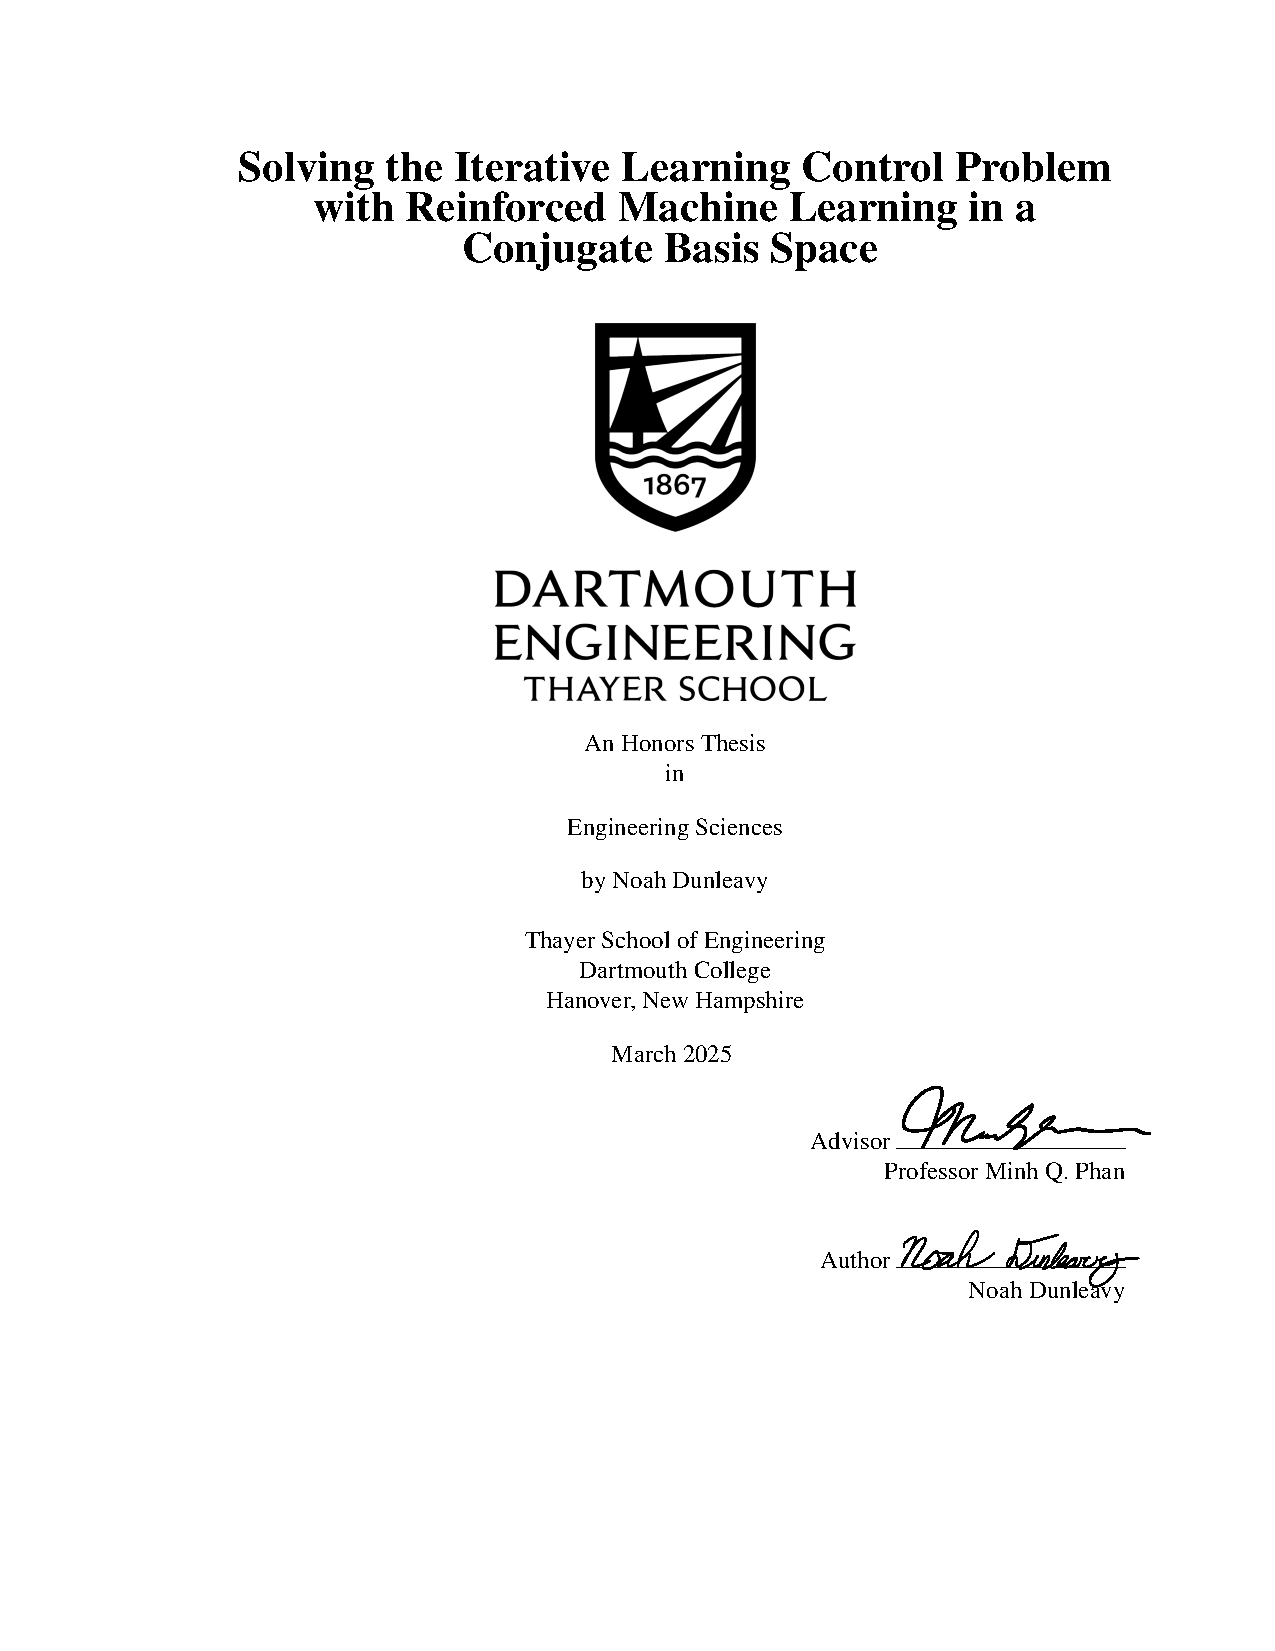
\includepdf[pages=1]{cover_page.pdf}
\newpage
% a blank page follows the title page, this page is not numbered
\mbox{}
\newpage

\renewcommand\thepage{\arabic{page}}
\pagenumbering{roman}        %% roman page numbers for front matterstarting with page ii
\setcounter{page}{2}

\doublespacing%              %% set spacing to double
\pagestyle{plain}
\begin{center}


\section*{ABSTRACT}


\end{center}

This abstract is included in your Thesis.  It should contain: Statement of problem, procedure or method, results and conclusions.  Max 350 words.

\cleardoublepage

\pagestyle{plain}
\begin{center}


\section*{Acknowledgements}
\addcontentsline{toc}{chapter}{Acknowledgements} 


\end{center}
This project could not have been accomplished without the help and support of so many incredible people.

I would like to start off by thanking Professor Phan. I took `ENGS26: Control Theory' with him in the Spring of my Sophomore year and by the end of the term had changed my major concentration. He presented topics in clear, understandable, and intuitive ways which I tried to replicate in this thesis. It was in his class `ENGS145: Modern Control Theory' where the base ideas for this Thesis were formed, and `ENGS149: System Identification' where I finally mustered the courage to ask him to be my advisor. I do not think a better mentor for a project such as this exists. I challenge you to find any other Professor who would be willing to stay around for hours on a Friday afternoon-turned-night to help work through proofs on the board, identify sources of errors, and provide paths forward for every problem that arose. It is my hope that the presented work is worthy of his time and dedication to my studies.

Next must come my partner Audrey Herrald. She has sat through hours of me frowning at a notebook, scratching at a chalkboard, banging at my keyboard, and generally thinking aloud - without complaint; all while going through Med School herself. She has heard all the material to follow more times than anyone, and has been a key figure of support to ensure I maintain priorities, focus, and sanity throughout this process.

The come my parents, Drs. Katherine and Keith Dunleavy. I have been truly fortunate in life to have the most amazing, loving, and supportive parents. All through my life, no matter what I did or how I did it, they have been there for me. Cheering me on from Little League to Robotics Competitions to Track Meets. No matter how much work I have ever had (or little I claimed to have), they provided me with every tool I needed to succeed. They have taught me through example what it means to work hard, take pride in what you do, and care for those around you. Mom, Dad - I love you.

Of course many others played their part in this process. My Grandparents - Ginghy and Grandad - for always checking in with me (and helping make sure I was never falling behind) and my sisters for letting me take over the entire kitchen table to do work. I would like to specifically Thank John DeForest, Alexander Zhelyazkov, and Emily Lukas for reading early drafts of my Introduction. 

Final thanks to all the friends and mentors who were with me along the way
\cleardoublepage%


\singlespacing%
\tableofcontents             %% include TOC
\listoffigures               %% include list of figures
\addcontentsline{toc}{chapter}{List of Figures}
%Warnings to suppress (manually decide for each file)
% chktex-file 8 %suppress warning about dash lengths

\chapter*{List of Acronyms and Variable Names}
\addcontentsline{toc}{chapter}{List of Acronyms and Variable Names} 

%Put in acronyms and the wordage used on variables (beta, y_bar, y_star, etc)

FISO - Full Input, Single Output
FIPO - Full Input, Partial Output
SIFO - Single Input, Full Output
PIFO - Partial Input, Full Output
$\Phi_u$, $\Phi_y$, $\eta_u$, $\eta_y$, $n_{ILC}$, just do everything tbh




\printglossary[type=acronym]


\cleardoublepage%             %% start new page

\pagenumbering{arabic}       %% arabic page numbers for body of text starting with page 1

\doublespacing%

\chapter{Introduction}
%Warnings to suppress (manually decide for each file)
% chktex-file 8 %suppress warning about dash lengths


\FloatBarrier\section{Purpose of Background} %Explanation of section
This section is dedicated to providing the base information of Modern Control Theory referenced in this Thesis.

To those familiar with the Thayer School of Engineering's curriculum, it is very similar to the content of ENGS145 - Modern Control Theory.

We begin with system formulation and representation in the matrix form, and how we resolve the difference between the continuous nature of the world, and the discrete ability of computers. Here, we use the \ac{ZOH} approach. 

Next the idea of pole placement is introduced, and it is demonstrated that the further from the origin the poles are, the longer control takes. A deadbeat controller is used to highlight this, which is the time-optimal solution for any system.

One will note that the deadbeat controller, while time optimal, requires significant control effort that may not be realistic or safe for a real system. That leads us to our introduction of the \ac{LQR} controller, which minimizes a cost function defined system inputs and states. 

Next we introduce the \ac{ILC} problem and show that it can learn to generate any output (so long as permitted by the physical characteristics of the system). 

Finally, we address the assumption of perfect knowledge not typically possible in the real world. The process of \ac{RL} is shown via the Policy Iteration and Input Decoupling method. They can be shown to find the \ac{LQR} controller as defined by its cost function. 

\FloatBarrier\section{Introduction to Continuous State Space} %Intro to State Space
A key step for Control Theory is construction of a system model, commonly represented as $A_c$, $B_c$, $C$ and $D$. $A_c$ captures the impact that the current state will have on the next state and $B_c$ captures how inputs will impact the next state. The matrix $C$ captures how states are translated to measured outputs and $D$ captures how inputs are directly measured on outputs. Any linear system, regardless of complexity and variations, can be modelled exactly as follows:

\begin{equation}
    \dot{x}(t) = A_c(t)x(t) + B_c(t)u(t) + \omega_x(t)
    \label{eq:continuous_state_space_model}
\end{equation}

\begin{equation}
    \dot{y}(t) = C(t)x(t) + D(t)u(t) + \omega_u(t)
    \label{eq:continuous_state_space_output}
\end{equation}

where $A_c(t)$, $B_c(t)$, $C(t)$, and $D(t)$ are the matrices describing the system dynamics, and the $\omega$ terms represent noise (like a residual in a regression). $x(t)$ is the state vector of dimensions $n\times1$, where $n$ is the number of states. There will be one state for every energy storing element in the system. $u(t)$ is the input vector of dimensions $r\times1$, where $r$ is the number of inputs. $y(t)$ is the output vector of dimensions $m\times1$, where $m$ is the number of outputs. As such, $A_c$ is $n\times n$, $B_c$ is $n\times r$, $C$ is $m\times n$ and $D$ is $m\times r$. Note that the matrices can be expressed in a time-variant form (a function of time), however for the entirety of this paper all matrices will be time-invariant. That is: $A_c\left(t\right)=A_c$ and the same goes for $B_c$, $C$, and $D$.

\subsection{Example --- State Space Formulation} %Example - Continuous Space
Most, if not all, of the world's physical systems can be modelled as a spring-mass-damper system. The mass and spring system that will be repeatedly referenced in this project is thus a dampened, two-mass-spring system, as seen in Fig~\ref{fig:spring_mass_system}

\begin{figure}[htbp] %try to place figure as close to this location as possible with htbp flag
    \centering  %center align
    \includegraphics[width=1\textwidth]{{latex_SMD.pdf}} %figure is as wide as text
    \caption{Dual Spring-Mass-Damper System}
~\label{fig:spring_mass_system}
\end{figure}

One can see that we have two masses, connected in series with springs and dampers, and bounded on one end with a wall. Constructing the equations of motion for the system simply follows Newton's second law $(F\ =\ ma)$, employing Hooke's $(F\ =\ -kx)$ and Damping Laws $(F=-cv)$. Recognizing that the derivative of position is velocity, and the derivative of velocity is acceleration, it can be shown that the equations of motion (EoM) for each mass are shown in Eqs.~\ref{eq:x1_eom} and~\ref{eq:x2_eom}.

\begin{equation}
    \begin{split}
        \ddot{x}_1(t) &= x_1(t)\left(\frac{-k_1-k_2}{m_1}\right) + x_2(t)\left(\frac{k_2}{m_1}\right) \\ 
        &+ \dot{x}_1(t)\left(\frac{-c_1-c_2}{m_1}\right)+\dot{x}_2(t)\left(\frac{c_2}{m_1}\right)+u_1(t)\left(\frac{1}{m_1}\right)
    \end{split}
    \label{eq:x1_eom}
\end{equation}

\begin{equation} 
    \begin{split}
        \ddot{x}_2(t) &= x_1(t)\left(\frac{k_2}{m_2}\right) + x_2(t)\left(\frac{-k_2}{m_2}\right) \\
        &+ \dot{x}_1(t)\left(\frac{c_2}{m_2}\right)+\dot{x}_2(t)\left(\frac{-c_2}{m_2}\right)+u_2(t)\left(\frac{1}{m_2}\right)
    \end{split}
    \label{eq:x2_eom}
\end{equation}

The next step is to select our `states'. For every energy-storing element in a system there will be one state. Our system stores energy as kinetic energy in the masses, and potential energy in the springs - we have four energy-storing elements and thus four states. It is most common and logical in spring-mass problems to select the position and velocity of the masses as these states:
\begin{equation} 
    x =
    \begin{bmatrix}
        x_1 \\ x_2 \\ \dot x_1 \\ \dot x_2
    \end{bmatrix}
    \label{eq:state_vector}
\end{equation}

Now for our inputs: these also are commonly and easily expressed as direct scalars of themselves. As such, our state vector and input vector is as follows:
\begin{equation} 
    u =
    \begin{bmatrix}
        u_1 \\ u_2
    \end{bmatrix}
    \label{eq:input_vector}
\end{equation}

Recall the idea of our model is to capture what the change in states will be, given current states and inputs. In the continuous format, the change in states is captured in the time derivative of the state vector, as shown in Eq.~\ref{eq:state_vector_derivative} below
\begin{equation} 
    \dot x =
    \begin{bmatrix}
        \dot x_1 \\ \dot x_2 \\ \ddot x_1 \\ \ddot x_2
    \end{bmatrix}
    \label{eq:state_vector_derivative}
\end{equation}

With all this matrix information, it is now time to construct our continuous state-space model of the form seen in Eq.~\ref{eq:continuous_state_space_model}. Through matrix multiplication we arrive upon the following:
\begin{equation} 
    \dot x =
    \begin{bmatrix}
        0 & 0 & 1 & 0 \\
        0 & 0 & 0 & 1 \\
        \frac{-k_1-k_2}{m_1} & \frac{k_2}{m_1} & \frac{-c_1-c_2}{m_1} & \frac{c_2}{m_1} \\
        \frac{k_2}{m_2} & \frac{-k_2}{m_2} & \frac{c_2}{m_2} & \frac{-c_2}{m_2}
    \end{bmatrix}
    x +
    \begin{bmatrix}
        0 & 0 \\
        0 & 0 \\
        \frac{1}{m_1} & 0 \\
        0 & \frac{1}{m_2}
    \end{bmatrix}
    u
    \label{eq:spring_mass_state_space_continuous}
\end{equation}

Recognizing this simple system is already messy, further substitutions can be made by formatting the masses, spring constants, and damping coefficients into a Mass (\ref{eq:mass_matrix}), Stiffness (\ref{eq:stiffness_matrix}), and Damping (\ref{eq:dampning_matrix}) Matrices. These are known as physical parameter matrices.
\begin{equation}
    M = 
    \begin{bmatrix}
        m_1 & 0 \\
        0 & m_2
    \end{bmatrix}
    \label{eq:mass_matrix}
\end{equation}
\begin{equation}
    K =
    \begin{bmatrix}
        k_1 + k_2 & -k_2 \\
        -k_2 & k_2
    \end{bmatrix}
    \label{eq:stiffness_matrix}
\end{equation}
\begin{equation}
    C = 
    \begin{bmatrix}
        c_1 + c_2 & -c_2 \\
        -c_2 & c_2
    \end{bmatrix}
    \label{eq:dampning_matrix}
\end{equation}

This would allow us to re-express our equations of motion in a single line as in Eq.~\ref{eq:compact_eom}
\begin{equation}
    \begin{bmatrix}
        \ddot{x}_1 \\ \ddot{x}_2
    \end{bmatrix}
    = M^{-1}K
    \begin{bmatrix}
        x_1 \\ x_2
    \end{bmatrix}
    + M^{-1}C
    \begin{bmatrix}
        \dot{x}_1 \\ \dot{x}_2
    \end{bmatrix}
    + M^{-1}
    \begin{bmatrix}
        u_1 \\ u_2
    \end{bmatrix}
    \label{eq:compact_eom}
\end{equation}

and our state-space model can now be written as
\begin{equation}
    \dot{x}=
    \begin{bmatrix}
        0_{2\times 2} & I_{2\times 2} \\
        -M^{-1}K & -M^{-1}C
    \end{bmatrix}
    x+
    \begin{bmatrix}
        0_{2\times 2} \\ -M^{-1}
    \end{bmatrix}
    u
    \label{eq:spring_mass_state_space_continuous_compact}
\end{equation}
This is exactly the format for the state-space model we described earlier in Eq.~\ref{eq:continuous_state_space_model}.
Now we put some numbers to our example so we can simulate behavior. We will define our system as follows
\begin{align}
    m_1 = 1\, \text{kg} \quad m_2 = 0.5\, \text{kg} \\
    k_1 = \frac{100\,\text{N}}{\text{m}} \quad k_2 = \frac{200\,\text{N}}{m} \\
    c_1 = \frac{1\,\text{Ns}}{m} \quad c_2 = \frac{0.5\,\text{Ns}}{m}
\end{align}
such that our physical parameter matrices are
\begin{equation}
    M = 
    \begin{bmatrix}
        1 & 0 \\
        0 & 0.5
    \end{bmatrix}
    \label{eq:mass_matrix_real}
\end{equation}
\begin{equation}
    K =
    \begin{bmatrix}
        300 & -200 \\
        -200 & 200
    \end{bmatrix}
    \label{eq:stiffness_matrix_real}
\end{equation}
\begin{equation}
    C = 
    \begin{bmatrix}
        1.5 & -0.5 \\
        -0.5 & 0.5
    \end{bmatrix}
    \label{eq:dampning_matrix_real}
\end{equation}

Plugging these values into Eq.~\ref{eq:spring_mass_state_space_continuous_compact}, we can write our system model as
\begin{equation} 
    \dot x =
    \begin{bmatrix}
        0 & 0 & 1 & 0 \\
        0 & 0 & 0 & 1 \\
        -300 & 200 & -1.5 & 0.5 \\
        400 & -400 & 1 & -1
    \end{bmatrix}
    x +
    \begin{bmatrix}
        0 & 0 \\
        0 & 0 \\
        1 & 0 \\
        0 & 2
    \end{bmatrix}
    u
    \label{eq:spring_mass_state_space_continuous_real}
\end{equation}

To explicitly complete the connection to Eq.~\ref{eq:continuous_state_space_model}, we can see
\begin{equation} 
    A_c =
    \begin{bmatrix}
        0 & 0 & 1 & 0 \\
        0 & 0 & 0 & 1 \\
        -300 & 200 & -1.5 & 0.5 \\
        400 & -400 & 1 & -1
    \end{bmatrix}
    \quad
    B_c = 
    \begin{bmatrix}
        0 & 0 \\
        0 & 0 \\
        1 & 0 \\
        0 & 2
    \end{bmatrix}
    \label{eq:Ac_Bc_real}
\end{equation}

We now only need one more piece of information to completely describe this system's behavior, and that is its initial conditions. We will choose to display the first mass one meter to the right of its' resting position and have the second mass moving to the right at two meters per second.
\begin{equation}
    x_0 =
    \begin{bmatrix}
        1 \\ 0 \\ 0 \\ 2
    \end{bmatrix}
    \label{eq:initial_conditions_real}
\end{equation}

Armed with the information to completely model the system, we now decide on our outputs. Recall Eq.~\ref{eq:continuous_state_space_output} relating the current state and inputs to the output, $y$ via matrices $C$ and $D$. For our system we will choose to only record the block positions ($x_1$ and $x_2$) as our outputs. Monitoring those two states 
is represented simply in matrix form
\begin{equation}
    y = 
    \begin{bmatrix}
        1 & 0 & 0 & 0 \\
        0 & 1 & 0 & 0
    \end{bmatrix}
    x +
    \begin{bmatrix}
        0 & 0 \\
        0 & 0
    \end{bmatrix}
    u
    \label{eq:continuous_output}
\end{equation}
where we will once again explicitly note
\begin{equation}
    C = 
    \begin{bmatrix}
        1 & 0 & 0 & 0 \\
        0 & 1 & 0 & 0
    \end{bmatrix}
    \quad D =
    \begin{bmatrix}
        0 & 0 \\
        0 & 0
    \end{bmatrix}
    \label{eq:C_D_real}
\end{equation}

The resulting outputs from simulation out this system can be seen in Fig.~\ref{fig:continuous_open_mass_1} and Fig.~\ref{fig:continuous_open_mass_2}
\begin{figure}[htbp]
    \centering  %center align
    \begin{subfigure}[b]{0.49\textwidth}
        \includegraphics[width=\textwidth]{{General Intro/Continuous Open-Loop - Mass 1.pdf}}
        \caption{}
        \label{fig:continuous_open_mass_1}
    \end{subfigure}
    \hfill
    \begin{subfigure}[b]{0.49\textwidth}
        \includegraphics[width=\textwidth]{{General Intro/Continuous Open-Loop - Mass 2.pdf}}
        \caption{}
        \label{fig:continuous_open_mass_2}
    \end{subfigure}
    \caption{Position data from a open-loop continuously-modelled Dual-Spring-Mass system}
\end{figure}

\FloatBarrier\section{Discretization of a Continuous Model} %Discretization
So far, we have been dealing with the ideal scenario of continuous time. While the models we constructed are exact, it is infeasible to collect outputs and apply inputs to a system at an infinite rate implied by a continuous model. Even if we were able to, it would be inefficient and impractical to run an infinite amount of calculations in an infinitely small time span. 
Digital systems fix this by discretizing their actions and outputs at a sampling rate denoted by $\Delta t$ (typically in units of seconds).  That is, every $\Delta t$ a new output is collected and input applied. To maintain the exact nature of the above model, matrices $A_c(t)$ and $B_c(t)$ must be `discretized' through the \ac{ZOH} method. The process for doing so is shown in Eqs.~\ref{eq:Ac_to_A} and~\ref{eq:Bc_to_B}
\begin{equation}
    A = e^{A_c \Delta t}
    \label{eq:Ac_to_A}
\end{equation}
\begin{equation}
    B = \int_{0}^{\Delta t}  e^{A_c \alpha}\,d\alpha B_c 
    \label{eq:Bc_to_B}
\end{equation}
What this relationship now constitutes is rather than applying instantaneous inputs, inputs are applied every $\Delta t$ and held for $\Delta t$. The response of the system between samples is not fully captured in the model, but at every discrete time step $k$ the model-to-nature relationship is exact. The output collection matrices $C$ and $D$ do not need to be adjusted. We can re-write our continuous state-space models from Eqs.~\ref{eq:continuous_state_space_model} and~\ref{eq:continuous_state_space_output} as
\begin{equation}
    x(k+1) = Ax(k) + Bu(k)
    \label{eq:discrete_state_space_model}
\end{equation}
\begin{equation}
    y(k) = Cx(k) + Du(k)
    \label{eq:discrete_state_space_output}
\end{equation}
An important notation distinction in discrete systems is the use of $k$ instead of a time value. $k$ represents discrete samples, occurring every $\Delta t$, but is unitless. To convert from a sample number $k$ to a continuous time, simply multiply the sample number by the sample rate.
\begin{equation}
    t = k \Delta t
    \label{eq:samples_to_time}
\end{equation}
As with all sampling and discretization, one must be wary of Nyquist sampling. A given system will have inherent `modes' - frequencies which it is easily excited and operates at. If your sampling rate $\Delta t$ is not sufficiently small, the exactness of the model will fail to capture crucial system dynamics.

Providing all the above steps and criteria are observed, we will be left with a model that exactly matches that of a continuous system, even in the presence of computational limits.

\FloatBarrier\subsection{Example --- Discretization} %Example - Discretization
Continuing with our earlier model, we now seek to discretize it for practical computational techniques. We will set $\Delta t=0.01$ seconds, and apply equations~\ref{eq:Ac_to_A} and~\ref{eq:Bc_to_B}. The resulting discrete matrices are
\begin{equation}
    A = 
    \begin{bmatrix}
        0.985&0.0099&0.0099&0.0001\\0.0198&0.9802&0.0001&0.0099\\-2.9398&1.9522&0.9704&0.0147\\3.9191&-3.9306&0.0295&0.9704
    \end{bmatrix}
    \quad
    B = 
    \begin{bmatrix}
        0&0\\0&0.0001\\0.0099&0.0001\\0.0001&0.0198
    \end{bmatrix}
    \label{eq:discrete_A_B}
\end{equation}
Note that in this perfect information scenario, we can verify our sufficient $\Delta t$ by examining the continuous-time system matrix $A_c$. The imaginary components of the eigenvalues are the natural frequencies of the system that $A_c$ describes. In our case, we have conjugate pairs with frequencies of 25.2 and 7.9 rad/sec. As we only care about the highest frequency (and sign does not matter), we convert 25.2 rad/sec to 4.0143 Hz. To avoid Nyquist sampling, we must sample at more than two times this rate, or over 8.0286 Hz. This corresponds with a sampling interval of 0.1246 seconds, which we are well below with our 0.01 second interval.

Now our system is captured in discrete form, as outlined in Eq.~\ref{eq:discrete_state_space_model}. Running that out and overlaying it with the results of the continuous system we arrive upon outputs depicted in Figures~\ref{fig:discrete_open_mass_1} and~\ref{fig:discrete_open_mass_2}.

\begin{figure}[htbp]
    \centering  %center align
    \begin{subfigure}[b]{0.49\textwidth}
        \includegraphics[width=\textwidth]{{General Intro/Open-Loop Mass 1 Position.pdf}}
        \caption{}%
        \label{fig:discrete_open_mass_1}
    \end{subfigure}
    \hfill
    \begin{subfigure}[b]{0.49\textwidth}
        \includegraphics[width=\textwidth]{{General Intro/Open-Loop Mass 2 Position.pdf}}
        \caption{}%
        \label{fig:discrete_open_mass_2}
    \end{subfigure}
    \caption{Position data from an open-loop discretely-modelled Dual-Spring-Mass system, overlaid with the continuous model to show exactness of the relationship}
\end{figure}

From this zoomed out view, it can be difficult to believe that the exact relationship does exist. Figures~\ref{fig:zoomed_discrete_open_mass_1} and~\ref{fig:zoomed_discrete_open_mass_2} step in to show that at every sampling interval of 0.01 seconds, the discrete model (outputs and states) match exactly that of the continuous one.

\begin{figure}[htbp]
    \centering  %center align
    \begin{subfigure}[b]{0.49\textwidth}
        \includegraphics[width=\textwidth]{{General Intro/Zoomed-in Open-Loop Mass 1 Position.pdf}}
        \caption{}%
        \label{fig:zoomed_discrete_open_mass_1}
    \end{subfigure}
    \hfill
    \begin{subfigure}[b]{0.49\textwidth}
        \includegraphics[width=\textwidth]{{General Intro/Zoomed-in Open-Loop Mass 2 Position.pdf}}
        \caption{}%
        \label{fig:zoomed_discrete_open_mass_2}
    \end{subfigure}
    \caption{Zoomed-in view of the discrete-continuous model to show that at the discretely modelled $\Delta t$ time-step samples, the relationship is exact}
\end{figure}

One thing to note -- moving forward, the discrete system model's x-axis will be expressed in terms of sample number $k$. For example, Figure~\ref{fig:zoomed_discrete_open_mass_1} axis will be marked with $k$ intervals 0 through 10, as opposed to time 0 through 0.1 seconds.

\FloatBarrier\section{Defining Control} %Control
With our model now modified to still be exact computationally, we can now proceed to do something with it. From a system model, it is now the goal to control the system. The simplest definition of `controlled' is once all states are zero -- this most classically is a system at rest. When the input to a system is some function of the system's states and/or outputs, we describe the system as `closed loop'. A typical controller demarcated by $F$ will be of dimensions $r\times n$ and is used to calculate inputs from collected data. As such, each input obeys the following control law when seeking stabilization (all states go to zero):
\begin{equation}
    u(k) = Fx(k)
    \label{eq:control_law}
\end{equation}
Following this control law, the state space equation in Eq.~\ref{eq:discrete_state_space_model} can be re-written as:
\begin{align}
    x(k+1)&=Ax(k)+BFx(k) \\
    &=(A+BF)x(k)
    \label{eq:A_BF_state_space}
\end{align}
A controlled system means that $x\left(k\right)=0$, so as $k$ goes to infinity, we would like $x\left(k\right)$ to go to zero. Any formulation of $A+BF$ that causes $x\left(k+1\right)$ to be smaller in magnitude than $x\left(k\right)$ will eventually result in an $x\left(k\right)=0$\footnote{Note that the controller depends only on the system matrices $A$ and $B$, and not at all on initial conditions}. In the scalar case this is easy to understand; suppose
\begin{equation}
    x(k+1)=\alpha x(k)
    \label{eq:scalar_control}
\end{equation}
Where $-1 < \alpha < 1$, then $\lim_{k \to \infty}{x(k) = 0}$. Taking this to a matrix-space preserves this intuition, only now instead of placing a scalar between -1 and 1, we seek to place the eigenvalues, or poles, of the system within the unit circle of the complex plane. Then regardless of any dynamics, a system will once again converge to zero. Poles placed at the boundary of the unit circle would denote an asymptotically stable system -- like a ball at the top of a hill, which will be stable until some force comes along and pushes it.
For any system defined by their $A$ and $B$ matrices, it is relevant to check if it is controllable. This is thankfully quite simple thanks to the Controllability Matrix. Defined as
\begin{equation}
    \mathcal{C}=\left[A^{\left(n-1\right)}B,\ldots,AB,B\right]
    \label{eq:controllability_matrix}
\end{equation}
If the Controllability Matrix $\mathcal{C}$ is full rank in rows, then the system is controllable (recall $n$ is the number of states). Full row rank means that no row of the matrix can be formulated through any linear combination of any of the other rows -- in other words, all rows are independent of one another\footnote{The same logic applies for full `column rank'}. If a matrix is said to be `full rank', then it will have a rank (number of linearly independent rows/columns) equal to its smallest dimension. So a full-rank $4 \times 2$ matrix will have rank of 2.

\FloatBarrier\subsection{Example --- Basic Control with Pole Placement} %Example - Pole Placement Control
There are practically an infinite number of controllers $F$ that could send our system to stability. The closer the poles are placed to the origin, the more rapid the convergence of the system will be. To illustrate this, we will first place the poles of our controlled moderately far from the origin, as seen in~\ref{fig:simple_poles}. Placement is done using MATLAB's \textit{place} function and then verified. Poles must always come in conjugate pairs, as visible in the reflection over the imaginary axis.
\begin{figure}[htbp]
    \centering
    \includegraphics[width=\textwidth]{{General Intro/Simple Pole Placement}}
    \caption{Pole locations for a Dual-Spring-Mass system when manually placed them at locations $0.5 +- 0.5i$ and $-0.7 +- 0.1i$}%
    \label{fig:simple_poles}
\end{figure}

The poles, placed at $0.5 +- 0.5i$ and $-0.7 +- 0.1i$ result in controller $F_{simple}$
\begin{equation}
    F_{simple} = 
    \begin{bmatrix}
        -40,364&-67,217&-161&-71\\5,468&7,726&-10&-73
    \end{bmatrix}
    \label{eq:simple_pole_controller}
\end{equation}
The way to interpret this controller (and framework for all future controllers) is best described with an example state, for which we will use our initial condition $x\left(0\right)$ as shown in Eq.~\ref{eq:initial_conditions_real}. The first row of the controller dictates how our first input ($u_1$ on $m_1$) is computed. In this case
\begin{equation}
    \begin{split}
        u_1\left(0\right)&=-40,364\cdot1+-67,217\cdot0+-161\cdot0+-71\cdot2\\
        &=-40,506
    \end{split}
    \label{eq:example_control_use_u0}
\end{equation}
The same process can be repeated for $u_2$ and for any sample number $k$. The way to verbalize a controller like this is as a state-input-weight relation, where the states are the columns, the inputs the rows, and the weight the corresponding value. For example, for every unit away from control $x_1$ is (recall `control' is a zero state), $u_1$ will generate -40,364 units of input. The net input will be the summed effects of each state.
When the controller in Eq.~\ref{eq:simple_pole_controller} is applied to our dual-mass system, our system produces outputs seen in Figs.~\ref{fig:simple_pole_mass_1} and~\ref{fig:simple_pole_mass_2}, under the inputs shown in Figs.~\ref{fig:simple_pole_input_1} and {\ref{fig:simple_pole_input_2}}

\begin{figure}[htbp]
    \centering  %center align
    \begin{subfigure}[b]{0.49\textwidth}
        \includegraphics[width=\textwidth]{{General Intro/Pole Placement - Mass 1 Position.pdf}}
        \caption{}%
       \label{fig:simple_pole_mass_1}
    \end{subfigure}
    \hfill
    \begin{subfigure}[b]{0.49\textwidth}
        \includegraphics[width=\textwidth]{{General Intro/Pole Placement - Mass 2 Position.pdf}}
        \caption{}%
        \label{fig:simple_pole_mass_2}
    \end{subfigure}
    \vfill
    \begin{subfigure}[b]{0.49\textwidth}
        \includegraphics[width=\textwidth]{{General Intro/Pole Placement - Input 1 Magnitude.pdf}}
        \caption{}%
        \label{fig:simple_pole_input_1}
    \end{subfigure}
    \hfill
    \begin{subfigure}[b]{0.49\textwidth}
        \includegraphics[width=\textwidth]{{General Intro/Pole Placement - Input 2 Magnitude.pdf}}
        \caption{}%
        \label{fig:simple_pole_input_2}
    \end{subfigure}
    \caption{Position of Mass 1 and Mass 2 for our Dual-Spring-Mass system under closed-loop, state-feedback controller $F$. $F$ is designed such that the poles of ($A+BF$) are at $0.5 +- 0.5i$ and $-0.7 +- 0.1i$. Inputs 1 and 2 are generated as $u(k) = Fx(k)$}
\end{figure}
\FloatBarrier~One will note that the system is stabilized after about twenty samples, or .2 seconds. The cost, however, is reflected in the inputs. What's known as the `control effort' applied is magnitudes more than the given state. This can be taken even further with a special type of controller known as a `deadbeat' controller. This is a controller which places the poles of a closed-loop system at the origin\footnote{MATLAB's \textit{place} function does not allow for multiple poles to be placed at the same location. Either use \textit{acker} or place poles very close to 0 ($\le 1\times 10^{-6}$)} and produces the time-optimal solution. Once again, the system poles are shown in Figure~\ref{fig:deadbeat_poles}
\begin{figure}[htbp]
    \centering
    \includegraphics[width=\textwidth]{{General Intro/Deadbeat Pole Placement}}
    \caption{Pole locations for a Dual-Spring-Mass system when manually placed them at the origin to produce a deadbeat controller}%
    \label{fig:deadbeat_poles}
\end{figure}
and produces controller $F_{deadbeat}$
\begin{equation}
    F_{deadbeat} =
    \begin{bmatrix}
        -9,800.7&-158&-148.8&-0.7\\-158&-4,841.9&-0.7&-74.3
    \end{bmatrix}
    \label{eq:deadbeat_controller}
\end{equation}
Its application results in the outputs and inputs denoted in Figures~\ref{fig:deadbeat_mass_1} -~\ref{fig:deadbeat_input_2}
\begin{figure}[htbp]
    \centering  %center align
    \begin{subfigure}[b]{0.49\textwidth}
        \includegraphics[width=\textwidth]{{General Intro/Deadbeat Controller - Mass 1 Position.pdf}}
        \caption{}%
       \label{fig:deadbeat_mass_1}
    \end{subfigure}
    \hfill
    \begin{subfigure}[b]{0.49\textwidth}
        \includegraphics[width=\textwidth]{{General Intro/Deadbeat Controller - Mass 2 Position.pdf}}
        \caption{}%
        \label{fig:deadbeat_mass_2}
    \end{subfigure}
    \vfill
    \begin{subfigure}[b]{0.49\textwidth}
        \includegraphics[width=\textwidth]{{General Intro/Deadbeat Controller - Input 1 Magnitude.pdf}}
        \caption{}%
        \label{fig:deadbeat_input_1}
    \end{subfigure}
    \hfill
    \begin{subfigure}[b]{0.49\textwidth}
        \includegraphics[width=\textwidth]{{General Intro/Deadbeat Controller - Input 2 Magnitude.pdf}}
        \caption{}%
        \label{fig:deadbeat_input_2}
    \end{subfigure}
    \caption{Position of Mass 1 and Mass 2 for our Dual-Spring-Mass system under a deadbeat closed-loop, state-feedback controller $F$. $F$ is designed such that the poles of ($A+BF$) are at $0$. Inputs 1 and 2 are generated as $u(k) = Fx(k)$. Under deadbeat control, it can be seen that control is achieved under $n$ steps}
\end{figure}

This pole placement method, while useful to demonstrate the requirements of a linear-feedback controller, is crude and often results in extreme states or inputs -- if not both. It would be useful then to be able to design a controller which can be tweaked more precisely to adhere to certain system limits.

\FloatBarrier\section{Linear Quadratic Regulator Controller} %\ac{LQR}
The \ac{LQR} Controller allows for the `weighting' of system states and inputs. What this means is that a controller can be designed that shies away from extreme inputs, at the cost of uncontrolled states, or conversely will take extreme steps to keep a system under control.
This is done by introducing three new variables: $Q$, $R$, and $\gamma$. $Q$ is an $n\times n$ matrix which applies relative `costs' (or rewards as desired) to states of the system. Similarly, $R$ is a $r\times r$ matrix which weighs the inputs. $\gamma$ is a scalar value between 0 and 1 which informs the cost function how much to discount the future versus the now (hence it is sometimes referred to as the `discount factor'). 
$Q$ and $R$ are then used to define the cost function we wish to minimize. It is most common to define them as identity matrices with some associated weight, but they truly can be set as whatever so long as they are symmetric ($Q=Q^T$ and $R=R^T$). We will only use the identity approach. What each component of the cost matrices $Q$ and $R$ tells us is how much cost to attribute to a component of the state or input, respectively, being away from zero. It is also important to note that weights are relative: a controller defined by $Q=100\cdot I_{n\times n}$ and $R=1\cdot I_{r\times r}$ will be the exact same as one defined by $Q=200\cdot I_{n\times n}$ and $R=2\cdot I_{r\times r}$.


Each sample, $k$, we want to have a scalar cost as a function of our states and inputs. For a given time step, we generate a utility function $U\left(k\right)$
\begin{equation}
    U\left(k\right)=u^T\left(k\right)Ru\left(k\right)+x^T\left(k\right)Q\ x\left(k\right)
    \label{eq:utility_function}
\end{equation}
In our journey to control, we will work through multiple time steps, each with their own $U\left(k\right)$, so in the whole process we will incur some net cost, $J$. The cost can be viewed as the summation of all these utilities along the way:
\begin{equation}
    J\ =\ \sum_{k=0}^{\infty}U\left(k\right)
    \label{eq:cost_function}
\end{equation}
Bringing back the aforementioned discount factor $\gamma$, we modify the cost function such that we can adjust the time horizon of consequence. Since $0<\gamma \le 1$, we can introduce it such that as $k$ goes to $\infty$, the impact of the infinite horizon utility reduces to zero. This is additionally useful as we want to be able to induce stability in finite-time. This presents us with our discounted cost function
\begin{equation}
    J\ =\ \sum_{k=0}^{\infty}{\gamma ^k U\left(k\right)}
    \label{eq:discounted_cost_function}
\end{equation}
In the LQR process, we are looking for a controller that minimizes the cost function, $J$.
The next important idea is the Principle of Optimality. Put simply, if the optimal path from Point A to point C goes through Point B, then the optimal path from Point B to Point C is a sub-set of the path from Point A to Point C. Figure~\ref{fig:principle_optimality} shows a two-step process: The red path from A to C through B is optimal (with minimum cost = 4 + 6 = 10). The principle of optimality states that if one starts from B then the optimal path to C must be the red path B-C. All other paths from B to C must cost more than 6, for example, the purple path that costs 10. The paths A-B1 and A-B2 cost less than the red path A-B, but the higher costs associated with their subsequent paths B1-C and B2-C result in higher total cost than the minimum cost. In addition, we can reason that all other paths from A to B such as the green path must cost more than 4. Otherwise, the statement that the red path A-B-C being the optimal path is contradicted. 
Image from \cite{Phan2025} - Chp8.
\begin{figure}[htbp]
    \centering
    \includegraphics[width=\textwidth]{{General Intro/Principal of Optimality - PhanChp8.png}}
    \caption{Illustration of Principle of Optimality, with nodes $A,\ B1,\ B2,\ B,\ $and $C$ with paths between labelled with their associated costs. Even though to go from $A \to B1$ is only a cost of $2$, $B1 \to C$ costs $12$ making the total path cost of $14$. Also see that the path of $A \to B2 \to C$ may have a final step of cost $1$, but the first step has a cost pf $15$. The central path through $B$ then could result in costs of $15,\ 14,\ 11,\ $or $10$. Clearly going through $B$ is the optimal way to proceed. It can then further be seen that the optimal way to go from $B \to C$ is a subset of the optimal path of $A \to C$.}
    \label{fig:principle_optimality}
\end{figure}


What this tells us is that no matter what step we are in a process, so long as we make the optimal step for that current state, we will be walking along the optimal path. It is not necessary to predict out any number of steps -- by making the best decision for this moment in time, the controller will set itself up to continue to make the most optimal decisions. Solving for the Discounted LQR Controller can be quite convoluted, but it can be shown to satisfy:
\begin{equation}
    F_{LQR}^\gamma=-\frac{1}{\sqrt\gamma}{\left(B^T PB+R_\gamma\right)}^{-1} B^T PA_\gamma
    \label{eq:discounted_LQR_solution}
\end{equation}
Where $R_\gamma=\frac{R}{\gamma}$,$A_\gamma=A\sqrt\gamma$, and $P$ is the solution to the algebraic Riccati equation associated with the un-discounted LQR problem
\begin{equation}
    P=A_\gamma^T PA_\gamma-A_\gamma^T PB{\left(R_\gamma+B^T PB\right)}^{-1}B^T PA_\gamma+Q
    \label{eq:LQR_solution}
\end{equation}


\FloatBarrier\subsection{Example --- LQR} %Example - LQR
It is now time to apply the logic of LQR to our system. To start, we must define our $Q$, $R$, and $\gamma$
\begin{equation}
    Q=100\cdot I_{4 \times 4} \quad R=1\cdot I_{2 \times 2} \quad \gamma=\ 0.8
    \label{eq:LQR_params_SMD}
\end{equation}
Using the attached function \textit{discount\_LQR}\footnote{MATLAB's dlqr function returns a different result than the one defined by our cost function as it does not have a discount parameter.} will find the correct controller for the cost function (and discount factor) we use. Applying that function to our discrete system, we find
\begin{equation}
    F_{LQR}=\left[\begin{matrix}9.9546&-1.8952&-2.6156&-0.3501\\-25.2185&29.3267&-0.8026&-3.767\\\end{matrix}\right]
    \label{eq:F_lqr}
\end{equation}
Examining where that places the poles (Figure~\ref{fig:big_Q_poles}) and the input-output data (Figures~\ref{fig:big_Q_mass_1} -~\ref{fig:big_Q_input_2}), we see that control takes almost two seconds, but inputs are magnitudes smaller than that seen by the pole placement controllers.

\begin{figure}[htbp]
    \centering
    \includegraphics[width=\textwidth]{{General Intro/Big Q LQR Pole Locations}}
    \caption{Pole Locations of a Q/R = 100 LQR Controller on our Dual-Spring-Mass System}%
    \label{fig:big_Q_poles}
\end{figure}
\begin{figure}[htbp]
    \centering  %center align
    \begin{subfigure}[b]{0.49\textwidth}
        \includegraphics[width=\textwidth]{{General Intro/Big Q LQR Controller - Mass 1 Position.pdf}}
        \caption{}%
       \label{fig:big_Q_mass_1}
    \end{subfigure}
    \hfill
    \begin{subfigure}[b]{0.49\textwidth}
        \includegraphics[width=\textwidth]{{General Intro/Big Q LQR Controller - Mass 2 Position.pdf}}
        \caption{}%
        \label{fig:big_Q_mass_2}
    \end{subfigure}
    \vfill
    \begin{subfigure}[b]{0.49\textwidth}
        \includegraphics[width=\textwidth]{{General Intro/Big Q LQR Controller - Input 1 Magnitude.pdf}}
        \caption{}%
        \label{fig:big_Q_input_1}
    \end{subfigure}
    \hfill
    \begin{subfigure}[b]{0.49\textwidth}
        \includegraphics[width=\textwidth]{{General Intro/Big Q LQR Controller - Input 2 Magnitude.pdf}}
        \caption{}%
        \label{fig:big_Q_input_2}
    \end{subfigure}
    \caption{Positions of Mass 1 and 2 under a state-feedback controller defined under LQR parameters of Q/R=100. Control is achieved within 200 samples, and under maximum input amplitudes of 55N}
\end{figure}

\myworries{Lip service to other pepers doing ILC and such - lit review}

\FloatBarrier~If we were inclined to tweak the parameters, perhaps the inputs were beyond the capabilities of our actual system, we could easily do so. If one were to scale $R$ by a factor of ten (or $Q$ by a factor of 0.1), then the following controller $F_{big R}$,  poles (Figure~\ref{fig:big_R_poles}), and IO data (Figures~\ref{fig:big_R_mass_1} -~\ref{fig:big_R_input_2}) would result:

\begin{equation}
    F_{big R} = 
    \begin{bmatrix}
        0.9118   & 0.1270 &  -0.3027 &  -0.0489\\
        -3.2549   & 3.8474  & -0.1148  & -0.4485
    \end{bmatrix}
\end{equation}

\begin{figure}[htbp]
    \centering
    \includegraphics[width=\textwidth]{{General Intro/Big R Pole Placement}}
    \caption{Pole Locations of a Q/R = 10 LQR Controller on our Dual-Spring-Mass System}%
    \label{fig:big_R_poles}
\end{figure}
\begin{figure}[htbp]
    \centering  %center align
    \begin{subfigure}[b]{0.49\textwidth}
        \includegraphics[width=\textwidth]{{General Intro/Big R LQR Controller - Mass 1 Position.pdf}}
        \caption{}%
       \label{fig:big_R_mass_1}
    \end{subfigure}
    \hfill
    \begin{subfigure}[b]{0.49\textwidth}
        \includegraphics[width=\textwidth]{{General Intro/Big R LQR Controller - Mass 2 Position.pdf}}
        \caption{}%
        \label{fig:big_R_mass_2}
    \end{subfigure}
    \vfill
    \begin{subfigure}[b]{0.49\textwidth}
        \includegraphics[width=\textwidth]{{General Intro/Big R LQR Controller - Input 1 Magnitude.pdf}}
        \caption{}%
        \label{fig:big_R_input_1}
    \end{subfigure}
    \hfill
    \begin{subfigure}[b]{0.49\textwidth}
        \includegraphics[width=\textwidth]{{General Intro/Big R LQR Controller - Input 2 Magnitude.pdf}}
        \caption{}%
        \label{fig:big_R_input_2}
    \end{subfigure}
    \caption{Positions of Mass 1 and 2 under a state-feedback controller defined under LQR parameters of Q/R=10. Control is achieved within 800 samples, and under maximum input amplitudes of 9N}
\end{figure}

It can be noted that stabilization takes much longer (around eight seconds), and the poles are much closer to the border of the unit circle. Setting $R=0_{2\times 2}$ logically does place poles at the unit circle, but it also places two at the unit circle border. This is because a deadbeat controller leads to extreme velocities -- a state we do not capture in the output but is factored into the cost. Without the presence of input weights, the controller solely focuses on states - all equally weighted in our case.

\FloatBarrier\section{Iterative Learning Control} %ILC
~\label{sec:ILC}
Switching gears, we will introduce now another form of system. The previous models have all been iterative in time (i.e.\ adjust next input based on last samples state), but there is a form of control that focuses on trials. This is logical for and applied in the manufacturing process, where the desired output is not a `zero' state, but rather zero error. \ac{ILC} is particularly useful for its ability to factor out repeated noise and function to produce machined outputs. This relies on the fact that in repeated tasks the initial conditions can be made to be repeated, even if they are not explicitly known\footfullcite{9374773}\footfullcite{4178138}.

Iterative Learning Control employs a system representation that is expanded to factor in the temporal element of control steps. Instead of each step ($k$) trying to send the states to zero, we now want each trial ($j$) to send the error on our outputs to zero\footfullcite{1636313}. 
The first step is to define our output, denoted as $\underline{y}$, occurring over p time steps. That is, y is a $pm\times 1$. Similarly, there is then a sequence of inputs, denoted as $\underline{u}$ that when applied, will get us here -- it will be $pr\times 1$. 

Finally, there exists a matrix $P$ that can be constructed out of $A$, $B$, $C$, and $D$ matrices such that the entire output captured from an input sequence can be represented as 
\begin{equation}
    \underline{y}=P\underline{u}+\underline{d}
    \label{eq:y_Pu_d}
\end{equation}
where $\underline{d}$ captures disturbances and initial conditions. All the above matrices are formulated as such
\begin{equation}
    \underline{y}=\left[\begin{matrix}y\left(1\right)\\y\left(2\right)\\\vdots\\y\left(p\right)\\\end{matrix}\right]
    \quad
    \underline{u}=\left[\begin{matrix}u\left(0\right)\\u\left(1\right)\\\vdots\\u\left(p-1\right)\\\end{matrix}\right]
    \label{eq:y_u_stacks}
\end{equation}
\begin{equation}
    P=\left[\begin{matrix}CB&D&0&0&0\\CAB&CB&D&0&0\\CA^2B&CAB&CB&\ddots&0\\\vdots&\vdots&\vdots&\ddots&D\\CA^{p-1}B&CA^{p-2}B&CA^{p-3}B&\cdots&CB\\\end{matrix}\right]
    \label{ILC_P}
\end{equation}
Note that in the ILC process we do not try to control $y\left(0\right)$ or even model it. We cannot control initial conditions and therefore do not worry about them.
As ILC is the pursuit of a desired output, we will mark that as ${\underline{y}}^ \ast $ and it stands that the input that gets us there is marked as ${\underline{u}}^ \ast $. That is:
\begin{equation}
    {\underline{y}}^\ast=P{\underline{u}}^\ast+\underline{d}
    \label{eq:y*_Pu*_d}
\end{equation}
The next step is to introduce the $\delta$ operator, signifying the difference between two value operations -- this can be thought of as a discrete derivative.
\begin{equation}
    \delta_j x=x_j-x_{j-1}
    \label{eq:delta_operator}
\end{equation}

Applying this $\delta$ operator to Eq.~\ref{eq:y_Pu_d}
\begin{equation}
    \delta_j\underline{y}=P\cdot\delta_j\underline{u}+\delta_j\underline{d}
    \label{eq:del_P_with_d}
\end{equation}
Recognizing $\underline{d}$ is a constant that does not change between trials allows us to drop it out of the equation to get
\begin{equation}
    \delta_j\underline{y}=P\cdot\delta_j\underline{u}
    \label{eq:del_y_P_del_u}
\end{equation}

Next, we define error. Each trial ($j$) will produce an output ${\underline{y}}_j$ that will be off from our goal out of ${\underline{y}}^\ast$ by an error denoted as
\begin{equation}
    e_j={\underline{y}}^\ast-{\underline{y}}_j
    \label{eq:e_j_def}
\end{equation}
Applying the $\delta$ operator to this equation
\begin{equation}
    \delta_j e=\delta_j{\underline{y}}^\ast-\delta_j\underline{y}
    \label{eq:del_e_law_w_star}
\end{equation}
Once again we have a constant (${\underline{y}}^\ast$) which drops out when the delta operator is applied. So 
\begin{equation}
    \delta_j e =-\delta_j \underline{y}
    \label{del_e_law}
\end{equation}
which expands to
\begin{equation}
    e_j-e_{j-1}=-\delta_j\underline{y}
    \label{e_j_e_j_1_law}
\end{equation}
To match our earlier notions of state-space models, we will increment every $j$ value by one (allowable since they are relative indices)
\begin{equation}
    e_{j+1}-e_j=-\delta_{j+1}\underline{y}
    \label{eq:e_j_1_e_law}
\end{equation}
Through re-arrangement of Eq.~\ref{eq:e_j_1_e_law} and substitution of Eq,~\ref{eq:del_y_P_del_u}, we arrive upon the ILC Equation
\begin{equation}
    e_{j+1}=Ie_j-P\delta_{j+1}\underline{u}
    \label{eq:ILC_law}
\end{equation}

This matches our earlier $A$, $B$ model except now $A$ is the identity matrix ($I$), and $B$ is the negative dynamics matrix $-P$. Additionally we now are dealing with `ILC States' ($n_{ILC}$) and `ILC Inputs' ($r_{ILC}$) and instead of control over samples, we control over trials. To send $e_j$ to zero as trials go to infinity, it is then desirable to find a controller of the form
\begin{equation}
    \delta_{j+1}\underline{u}=\mathcal{L}e_j
    \label{eq:del_u_L_e_j}
\end{equation}
Where $\mathcal{L}$ is $pr\times pm$ (or $r_{ILC} \times n_{ILC}$). As we have already explored the ideas of controllers, it logically follows there are an infinite number of these controllers, all facing tradeoffs. 

\FloatBarrier\subsection{Example --- ILC} %Example - ILC
The first step in setting up an ILC problem is to establish the goal, or $y^\ast$. For simplicity, we will work through this example trying to draw a circle. That is, $x_1$ would ideally trace out one period of a cosine, and $x_2$ will follow one period of a sine wave. We can set the resolution of this circle by our choice of $p$.
Supposed we set $p=100$, meaning we want to draw a circle over $p$ discrete time steps. We will define the goal for our first output (the position of $x_1$) as $y_1^\ast$ and the second output (position of $x_2$) as $y_2^\ast$:
\begin{equation}
    y_1^\ast=\cos\left(\frac{2\pi k}{p}\right)
    \quad
    y_2^\ast=\sin\left(\frac{2\pi k}{p}\right)
    \label{eq:y1_y2_star}
\end{equation}
Combining those into $y^\ast$ produces the goal we mark each trial against. It is very important to recognize that $y^\ast$ is an alternating stack of the component goals
\begin{equation}
    {\underline{y}}^\ast=\left[\begin{matrix}y_1^\ast\left(1\right)\\y_2^\ast\left(1\right)\\\vdots\\y_1^\ast\left(p\right)\\y_2^\ast\left(p\right)\\\end{matrix}\right]
    \label{eq:stacked_y_star}
\end{equation}
With our goal in hand, we now choose a controller. As earlier illustrated, the only requirement of the controller is to place the poles of the system in the unit circle. Now instead of $\left(A+BF\right)$ determining the location of our poles however, it is $\left(I-P\mathcal{L}\right)$. By selecting a controller to be $\mathcal{L}=\alpha P^+$ (where + denotes the pseudo inverse operation and $0<\ \alpha<1$), we can guarantee such pole placement. For the presented system, we select $\alpha=\ 0.8$, which we will apply for just 10 trials
\begin{equation}
    \mathcal{L} = 0.8P^+
    \label{eq:ilc_controller}
\end{equation}

Plotting the normalization of the error term for each trial, scaled down by the number of outputs in each trial, we can see below that the error rapidly drops to zero.
\begin{figure}
    \centering
    \includegraphics[width=\textwidth]{{General Intro/Placed Controller ILC - Error Progression}}
    \caption{Error Progression of an ILC problem when using a perfect knowledge controller $\mathcal{L} = 0.8P^+$ such that the poles of the system under ($I-P\mathcal{L}$) are guaranteed to be within the unit circle and relatively close to the origin for rapid convergence.}%
    \label{fig:ilc_error}
\end{figure}

Further showing the progression of the individual outputs and inputs (Figures~\ref{fig:ilc_mass_1} -~\ref{fig:ilc_input_2}) as well as the shaped output in Figure~\ref{fig:ilc_shaped_circle} (where $x_1$'s position is the x-axis and $x_2$'s position is the y-axis), you can see as the system `learns' to draw the circle. Trial 1 matches our open-loop response, but even Trial 2 much more closely matches our goal (marked by the dotted red line). It is convenient here that the initial conditions of the system match those of the initial goal outputs, but we will shortly show that it is not necessary.

\begin{figure}[htbp]
    \centering  %center align
    \begin{subfigure}[b]{0.49\textwidth}
        \includegraphics[width=\textwidth]{{General Intro/Placed Controller ILC - Mass 1 Position.pdf}}
        \caption{}%
       \label{fig:ilc_mass_1}
    \end{subfigure}
    \hfill
    \begin{subfigure}[b]{0.49\textwidth}
        \includegraphics[width=\textwidth]{{General Intro/Placed Controller ILC - Mass 2 Position.pdf}}
        \caption{}%
        \label{fig:ilc_mass_2}
    \end{subfigure}
    \vfill
    \begin{subfigure}[b]{0.49\textwidth}
        \includegraphics[width=\textwidth]{{General Intro/Placed Controller ILC - Input 1.pdf}}
        \caption{}%
        \label{fig:ilc_input_1}
    \end{subfigure}
    \hfill
    \begin{subfigure}[b]{0.49\textwidth}
        \includegraphics[width=\textwidth]{{General Intro/Placed Controller ILC - Input 2.pdf}}
        \caption{}%
        \label{fig:ilc_input_2}
    \end{subfigure}
    \caption{The progression of Input-Output trials under our controller of $\mathcal{L} = 0.8P^+$. Trial 1 can be seen to be the open-loop response, and by Trial 10 it can be seen that the output is captured with zero error}
\end{figure}
\begin{figure}[htbp]
    \centering
    \includegraphics[width=\textwidth]{{General Intro/Placed Controller ILC - Shaped Output.pdf}}
    \caption{Progression of shaped outputs (where Mass 1 Position is the x-coordinate and Mass 2 Position is the y-coordinate) under our ILC controller $\mathcal{L} = 0.8P^+$}%
    \label{fig:ilc_shaped_circle}
\end{figure}

\FloatBarrier~To demonstrate ILC's ability to learn arbitrary shapes, a $p=500$ point resolution, mouse-drawn version of the word `Dartmouth' was introduced as the ${\underline{y}}^\ast$. Utilizing the same controller shown in Eq.~\ref{eq:ilc_controller}, we can similarly learn the exact inputs required to generate our desired output. The sharp jump from the starting position (1, 0) is the point $(y_1\left(0\right),y_2\left(0\right))$ which we have previously mentioned we cannot control. As such, the ${\underline{y}}^\ast$ does not start at that point, but rather at the green `play' symbol
\begin{figure}[htbp]
    \centering
    \includegraphics[width=\textwidth]{{General Intro/Dartmouth ILC - Shaped Output.pdf}}
    \caption{Application of ILC Controller $\mathcal{L} = 0.8P^+$ on our Dual-Spring-Mass system to learn the output `Dartmouth'. It can be seen that initial conditions and arbitrariness of different goals has no impact on the efficacy of ILC}%
    \label{fig:ilc_shaped_dartmouth}
\end{figure}
\begin{figure}[htbp]
    \centering  %center align
    \begin{subfigure}[b]{0.49\textwidth}
        \includegraphics[width=\textwidth]{{General Intro/Dartmouth ILC - Mass 1 Position.pdf}}
        \caption{}%
        \label{fig:dartmouth_ilc_mass_1}
    \end{subfigure}
    \hfill
    \begin{subfigure}[b]{0.49\textwidth}
        \includegraphics[width=\textwidth]{{General Intro/Dartmouth ILC - Mass 2 Position.pdf}}
        \caption{}%
        \label{fig:dartmouth_ilc_mass_2}
    \end{subfigure}
    \caption{Progression of Mass 1 and 2 Positions under controller $\mathcal{L} = 0.8P^+$, learning `Dartmouth'. It can be seen that Mass 1, the x-position, gradually increases throughout the each trial whereas Mass 2, the y-position, simply moves back-and-forth / up-and-down}
\end{figure}

\FloatBarrier\section{Reinforcement Learning} %RL
Until now we have been assuming that we always know the $A,\ B,\ C$, and $D$ matrices. This is a bold assumption, not often matched in reality. It is then desirable to be able to construct a model-free controller for a given system.
Recall our earlier cost function seen in Eq.~\ref{eq:discounted_cost_function}. We can choose to restrict our time horizon down from infinity, and now look $s$ steps ahead. We can then create a cost-to-go function $V(k)$:
\begin{equation}
    V\left(k\right)=\sum_{i=0}^{s-1}{\gamma^i U\left(k+1\right)=U\left(k\right)+\gamma U\left(k+1\right)+\cdots+\gamma^{s-1}U\left(k+s-1\right)}
    \label{eq:cost_to_go}
\end{equation}
As from our principle of optimality, it similarly follows that whatever controller minimizes $V\left(k\right)$ will then also minimize $J$. This agrees with an important feature of the cost-to-go function, and that is recurrence. If we multiply Eq.~\ref{eq:cost_to_go} by $\gamma$ and increment $k$ by 1, we get
\begin{equation}
    \gamma V\left(k+1\right)=\gamma U\left(k+1\right)+\cdots+\gamma^s U\left(k+s\right)
    \label{eq:gamma_inc_cost_to_go}
\end{equation}
Substituting Eq.~\ref{eq:gamma_inc_cost_to_go} into~\ref{eq:cost_to_go}, the relationship between $V\left(k\right)$ and $V\left(k+1\right)$ can be shown
\begin{equation}
    V\left(k\right)=\gamma V\left(k+1\right)+U\left(k\right)-\gamma^s U\left(k+s\right)
    \label{eq:expanded_recurrence}
\end{equation}
This is known as the recurrence equation. So long as $\gamma<\ 1$ and $s$ is sufficiently large,
\begin{equation}
    V\left(k\right)=\gamma V\left(k+1\right)+U\left(k\right)
    \label{eq:recurrence}
\end{equation}
It can then be useful to express $V\left(k\right)$ in a supervector format for later descriptions and derivations. Substituting the utility function described in Eq.~\ref{eq:utility_function} into Eq.~\ref{eq:expanded_recurrence}
\begin{equation}
    \begin{split}
        V\left(k\right)&=u^T\left(k\right)Ru\left(k\right)+x^T\left(k\right)Qx\left(k\right) \\
        &+\gamma u^T\left(k+1\right)Ru\left(k+1\right)+\gamma x^T\left(k+1\right)Qx\left(k+1\right) \\
        & + \cdots + \\
        &+\gamma^{s-1}u^T\left(k+s-1\right)Ru\left(k+s-1\right) \\
        &+\gamma^{s-1}x^T\left(k+s-1\right)Qx\left(k+s-1\right)
    \end{split}
    \label{eq:supervector_expanded_ctg}
\end{equation}
And we can define supervectors for state and input histories
\begin{equation}
    x_s\left(k\right)=\left[\begin{matrix}x\left(k\right)\\x\left(k+1\right)\\\vdots\\x\left(k+s-1\right)\\\end{matrix}\right]	
    \quad
    u_s\left(k\right)=\left[\begin{matrix}u\left(k\right)\\u\left(k+1\right)\\\vdots\\u\left(k+s-1\right)\\\end{matrix}\right]
    \label{eq:supervector_state_input}
\end{equation}
It is further beneficial to define matrices $\textbf{Q}_\gamma=\Lambda_n\textbf{Q}\Lambda_n$ and $\textbf{R}_\gamma=\Lambda_r\textbf{R}\Lambda_r$, where Q and R are $ns\ \times ns$ and $rs\times rs$ block-diagonal matrices comprised of $s$ of the cost-defining matrices $Q$ and $R$ (respectively)
\begin{equation}
    \textbf{Q}\ =\ \left[\begin{matrix}Q_{n\times n}&0&0\\0&\ddots&0\\0&0&Q_{n\times n}\\\end{matrix}\right]
    \quad
    \textbf{R}\ =\ \left[\begin{matrix}R_{r\times r}&0&0\\0&\ddots&0\\0&0&R_{r\times r}\\\end{matrix}\right]
    \label{eq:QR_supervector}
\end{equation}
and the $\Lambda$ matrices are defined as
\begin{equation}
    \Lambda_n=\left[\begin{matrix}I_{n\times n}&&&\\&\sqrt\gamma I_{n\times n}&&\\&&\ddots&\\&&&{\left(\sqrt\gamma\right)}^{s-1}I_{n\times n}\\\end{matrix}\right]
    \label{eq:lambda_n}
\end{equation}
\begin{equation}
    \Lambda_r=\left[\begin{matrix}I_{r\times r}&&&\\&\sqrt\gamma I_{r\times r}&&\\&&\ddots&\\&&&{\left(\sqrt\gamma\right)}^{s-1}I_{r\times r}\\\end{matrix}\right]
    \label{eq:lambda_r}
\end{equation}

Now Eq.~\ref{eq:supervector_expanded_ctg} can be re-written as
\begin{equation}
    V\left(k\right)=u_s^T\left(k\right)\textbf{R}_\mathbf{\gamma}u_s\left(k\right)+x_s^T\left(k\right)\textbf{Q}_\mathbf{\gamma}{x}_{s}\left({k}\right)
    \label{eq:supervector_ctg}
\end{equation}

The above formulations make it easier to now represent our Q-function. The Q-function is defined by the current state and input of a system and defined with respect to a controller $F$. Its logic is as follows: suppose we are at state $x\left(k\right)$ and have just made input $u\left(k\right)$ -- both can be arbitrary. However, from time k+1 to infinity, our next state $(x(k+1),\ x(k+2),\ \ldots)$ will be a function of our previous state and input, as described in Eq.~\ref{eq:discrete_state_space_model}. And our inputs $(u(k+1),\ u(k+2),\ \ldots)$ will follow the control law described in Eq.~\ref{eq:control_law}. Thus the vector $x_s\left(k\right)$ can be expressed in terms of the current state $x\left(k\right)$, the current input $u\left(k\right)$, and all future inputs to $u\left(k+s-1\right)$ as
\begin{equation}
    x_s\left(k\right)=P_1x\left(k\right)+P_2u_s\left(k\right)
    \label{eq:xs}
\end{equation}
where
\begin{equation}
    P_1=\left[\begin{matrix}I\\A\\\vdots\\A^{s-1}\\\end{matrix}\right]	
    \quad
    P_2=\left[\begin{matrix}0&&&\\B&0&&\\\vdots&\ddots&\ddots&\\A^{s-2}B&\cdots&B&0\\\end{matrix}\right]
    \label{eq:P1_P2}
\end{equation}
Substituting these into our cost-to-go expression of Eq.~\ref{eq:supervector_ctg}, we get a cost-to-go defined only in terms of present state and all inputs from now until $s$
\begin{equation}
    V\left(k\right)=u_s^T\left(k\right)\mathbf{R}_\mathbf{\gamma}u_s\left(k\right)+{\left[P_1x\left(k\right)+P_2u_s\left(k\right)\right]}^T\textbf{Q}_\gamma\left[P_1x\left(k\right)+P_2u_s\left(k\right)\right]
\end{equation}
If we define the symmetric matrix $\textbf{S}$ as
\begin{equation}
    \textbf{S}\ =\ \left[\begin{matrix}P_1^T\textbf{Q}_\gamma P_1&P_1^T\textbf{Q}_\gamma P_2\\P_2^T\textbf{Q}_\gamma P_1&\textbf{R}_\gamma+P_2^T\textbf{Q}_\gamma P_2\\\end{matrix}\right]
\end{equation}
We can once again reduce the cost-to-go function to
\begin{equation}
    V\left(k\right)={\left[\begin{matrix}x\left(k\right)\\u_s\left(k\right)\\\end{matrix}\right]}^T\textbf{S}\left[\begin{matrix}x\left(k\right)\\u_s\left(k\right)\\\end{matrix}\right]
    \label{eq:xus_cost_to_go}
\end{equation}
As previously mentioned, all inputs after k will follow the control law $u\left(k\right)=Fx\left(k\right)$, and so it must be possible to further reduce our representation. Start with
\begin{equation}
    u_s\left(k\right)=\left[\begin{matrix}u\left(k\right)\\u_{s-1}\left(k+1\right)\\\end{matrix}\right]	
    \quad
    u_{s-1}\left(k+1\right)=\left[\begin{matrix}u\left(k+1\right)\\u\left(k+2\right)\\\vdots\\u\left(k+s-1\right)\\\end{matrix}\right]
    \label{eq:u_s_and_u_s_1}
\end{equation}
Given our system model and control law, all future inputs can be tracked back to $x\left(k\right)$ and $u\left(k\right)$. By repeated substitution, it can be shown
\begin{align}
    u(k+1) &= Fx(k+1) = F\left[Ax(k) + Bu(k)\right] \nonumber \\
    u(k+2) &= Fx(k+2) = F(A+BF)\left[Ax(k) + Bu(k)\right] \nonumber \\
    &\; \vdots  \\
    u(k+s-1) &= F{(A+BF)}^{s-2} \left[Ax(k) + Bu(k)\right] \nonumber
    \label{eq:u_dynamics}
\end{align}

We can now rewrite~\ref{eq:u_s_and_u_s_1}  as
\begin{equation}
    u_{s-1}\left(k+1\right)=F_{xx}\left(k\right)+F_{uu}\left(k\right)
\end{equation}
where
\begin{equation}
    F_x=\left[\begin{matrix}FA\\F\left(A+BF\right)A\\\vdots\\{F\left(A+BF\right)}^{s-2}A\\\end{matrix}\right]
    \quad
    F_u=\left[\begin{matrix}FB\\F\left(A+BF\right)B\\\vdots\\F{\left(A+BF\right)}^{s-2}B\\\end{matrix}\right]
\end{equation}

Then
\begin{equation}
    \left[\begin{matrix}x\left(k\right)\\u_s\left(k\right)\\\end{matrix}\right]=\left[\begin{matrix}x\left(k\right)\\u\left(k\right)\\u_{s-1}\left(k+1\right)\\\end{matrix}\right]=\left[\begin{matrix}I_{n\times n}&0_{n\times r}\\0_{r\times n}&I_{r\times r}\\F_x&F_u\\\end{matrix}\right]\left[\begin{matrix}x\left(k\right)\\u\left(k\right)\\\end{matrix}\right]
\end{equation}

Defining \textbf{R}
\begin{equation}
    \textbf{R}=\left[\begin{matrix}I_{n\times n}&0_{n\times r}\\0_{r\times n}&I_{r\times r}\\F_x&F_u\\\end{matrix}\right]
\end{equation}
We can now write
\begin{equation}
    \left[\begin{matrix}x\left(k\right)\\u_s\left(k\right)\\\end{matrix}\right]=\textbf{R}\left[\begin{matrix}x\left(k\right)\\u\left(k\right)\\\end{matrix}\right]
    \label{eq:xus_to_Rxu}
\end{equation}
If we create matrix\footnote{Note this is not the same P matrix defined in the ILC problem} P = $\textbf{R}^{T}$\textbf{SR}, we can substitute Eq.~\ref{eq:xus_to_Rxu} into Eq.~\ref{eq:xus_cost_to_go} to get a new cost-to-go function
\begin{equation}
    Q\left(x\left(k\right),u\left(k\right)\right)={\left[\begin{matrix}x\left(k\right)\\u\left(k\right)\\\end{matrix}\right]}^T\textbf{P}\left[\begin{matrix}x\left(k\right)\\u\left(k\right)\\\end{matrix}\right] 
    \label{eq:q_function}
\end{equation}
We may now utilize this formulation, along with the recurrence equation, to find the optimal Q-function. As the Q-function is defined for a given controller $F$, and we constructed $Q\left(x\left(k\right),u\left(k\right)\right)$ in our observance with the cost function that defined our LQR controller, the Q-function will be optimized by the LQR controller.
The optimal controller $F$ will produce $u\left(k+1\right)$ that minimizes our cost-to-go, now defined in Eq.~\ref{eq:q_function}, starting from $x\left(k\right)$. That is, it will give us input $u\left(k+1\right)$ defined as:
\begin{equation}
    u(k+1)=\arg{\min_{u\left(k+1\right)}}Q(x(k+1), u(k+1))
\end{equation}
A comment on the `argmin' function: this operator will give us the value of the specified argument that will minimize the given function. So in our case, the $u\left(k+1\right)$ that will minimize the cost-to-go function $Q\left(x\left(k+1\right),u\left(k+1\right)\right)$ is returned. Therefore it follows that the Q-function that utilizes this minimizing input will equal the minimum possible value for the Q-function
\begin{equation}
    Q(x(k+1), \arg{\min_{u\left(k+1\right)}}Q(x(k+1), u(k+1)))=\min_{u\left(k+1\right)}Q(x(k+1), u(k+1))
    \label{eq:q_function_min_recurrence}
\end{equation}
So we can now write the recurrence equation for the deterministic Q-Learning-based RL method. By taking Eq.~\ref{eq:recurrence}, substituting in our new cost-to-go defined in Eq.~\ref{eq:q_function} and the logic in Eq.~\ref{eq:q_function_min_recurrence}, we arrive upon the relationship that the optimal Q-function (as defined by the optimal controller) must satisfy:
\begin{equation}
    Q\left(x\left(k\right),u\left(k\right)\right)=\gamma \min_{u\left(k+1\right)}{Q\left(x\left(k+1\right),u\left(k+1\right)\right)+U\left(k\right)}
    \label{eq:optimal_q_recurrence}
\end{equation}
Any Q-function will satisfy
\begin{equation}
    Q\left(x\left(k\right),u\left(k\right)\right)=\gamma Q\left(x\left(k+1\right),u\left(k+1\right)\right)+U\left(k\right)
    \label{eq:q_recurrence}
\end{equation}
but only Eq.~\ref{eq:optimal_q_recurrence} is satisfied by the optimal Q-function, as defined by the optimal controller $F$.

To extract the controller from a given Q-function, we return to Eq.~\ref{eq:q_function}. Recall matrix \textbf{P} is symmetric. We can re-write it as
\begin{equation}
    \textbf{P}=\left[\begin{matrix}\textbf{P}_{xx}&\textbf{P}_{xu}\\{\textbf{P}_{xu}}^T&\textbf{P}_{uu}\\\end{matrix}\right]
    \label{eq:sym_P_rl}
\end{equation}
Where the $x$ and $u$ subscript indicate the size of each \textbf{P} component.\ \textbf{P} is $\left(n+r\right)\times \left(n+r\right)$, so $\textbf{P}_{xx}$ refers to the top-left $n \times n$ portion, and the same logic follows for the other components. We can extract controller $F$ as
\begin{equation}
    F=-{\left(\textbf{P}_{uu}\right)}^{-1}\left(\textbf{P}_{xu}^T\right)
    \label{eq:F_from_P}
\end{equation}
Thus we have shown from a Q-function we can extract its controller, and given that we have an equation of recurrence that defines the optimal Q-function, we can begin to solve for the optimal Q-function purely from system input-output data.

\FloatBarrier\subsection{Policy Iteration} %Policy Iteration
The first method which we will demonstrate is that of Policy Iteration. To do this, we need data triplets of $x\left(k\right),u\left(k\right)$ and $x\left(k+1\right)$. By manipulating enough of these triplets, we can episodically solve for the \textbf{P} that parametrizes a Q-function, while simultaneously optimizing the Q-function. We begin with Eq.~\ref{eq:q_recurrence}, but re-arrange it to
\begin{equation}
    Q\left(x\left(k\right),u\left(k\right)\right) - \gamma Q\left(x\left(k+1\right),u\left(k+1\right)\right)=U\left(k\right)
    \label{eq:q-gamma_q}
\end{equation}
It is next necessary to find a way to re-write $Q\left(x\left(k\right),u\left(k\right)\right)$. 
We will start by defining the stack operator for a matrix. Given an arbitrary matrix $H$ that is $v\times w$, the stack operator creates $H^s$ that is a single column, making our matrix $vw \times1$. So if
\begin{equation}
    H = \left[\begin{matrix}h_1&h_2&\cdots&h_w\\\end{matrix}\right]
    \label{eq:H_prestack}
\end{equation}
Where each $h_i$ is $v\times1$, then
\begin{equation}
    H^S=\left[\begin{matrix}h_1\\h_2\\\vdots\\h_w\\\end{matrix}\right]
    \label{eq:H_stacked}
\end{equation}
It is important to recognize that the stack operator is \underline{not} the transpose operation, as each $h_i$ is a vector, not a scalar.
Our next operator is the Kronecker product, marked $\otimes$. This operator is used to multiply two matrices in a way such that each component of one is used to scale the entirety of the second. So for an $m \times n$ matrix $A$, and a $p \times q$ matrix $B$
\begin{equation}
    A\ =\ \left[\begin{matrix}a_{11}&\cdots&a_{1n}\\\vdots&\ddots&\vdots\\a_{m1}&\cdots& a_{mn}\\\end{matrix}\right]	
    \quad
    B=\left[\begin{matrix}b_{11}&\cdots&b_{1q}\\\vdots&\ddots&\vdots\\b_{p1}&\cdots&b_{pq}\\\end{matrix}\right]
\end{equation}
The Kronecker product between the two will create an $mp \times nq$ matrix
\begin{equation}
    A\ \otimes B\ =\ \left[\begin{matrix}a_{11}B&\cdots&a_{1n}B\\\vdots&\ddots&\vdots\\a_{m1}B&\cdots&a_{mn}B\\\end{matrix}\right]
\end{equation}
Now to see how these operators will be useful, we return to Eq.~\ref{eq:q_function}, re-written below as
\begin{gather}
    Q\left(x\left(k\right),u\left(k\right)\right)={\left[\begin{matrix}x\left(k\right)\\u\left(k\right)\\\end{matrix}\right]}^T\textbf{P}\left[\begin{matrix}x\left(k\right)\\u\left(k\right)\\\end{matrix}\right] \tag{\ref{eq:q_function}}
\end{gather}
To better demonstrate the process, we will assume $x\left(k\right)$ and $u\left(k\right)$ are scalar, and \textbf{P} is thus a $2\times 2$ matrix. 
\begin{equation}
    {x}\left(k\right)=x_1
    \quad
    u\left(k\right)=u_1
    \quad
    \textbf{P}=\left[\begin{matrix}\textbf{P}_{11}&\textbf{P}_{12}\\\textbf{P}_{21}&\textbf{P}_{22}\\\end{matrix}\right]
\end{equation}
Manually working out Eq.~\ref{eq:q_function}, we can re-write it as
\begin{equation}
    \begin{split}
        Q\left(x\left(k\right),u\left(k\right)\right)=\left[\begin{matrix}x_1&u_1\\\end{matrix}\right]\left[\begin{matrix}\textbf{P}_{11}&\textbf{P}_{12}\\\textbf{P}_{21}&\textbf{P}_{22}\\\end{matrix}\right]\left[\begin{matrix}x_1\\u_1\\\end{matrix}\right] \\
        =\left[\begin{matrix}x_1\textbf{P}_{11}+u_1\textbf{P}_{21}&x_1\textbf{P}_{12}+u_1\textbf{P}_{22}\\\end{matrix}\right]\left[\begin{matrix}x_1\\u_1\\\end{matrix}\right] \\
        =x_1^2\textbf{P}_{11}+x_1u_1\textbf{P}_{21}+x_1u_1\textbf{P}_{12}+u_1^2\textbf{P}_{22}
    \end{split}
    \label{eq:manual_Q_ex}
\end{equation}
It can be shown that the results of Eq.~\ref{eq:manual_Q_ex} can then be expressed by stacking \textbf{P} as
\begin{equation}
    Q\left(x\left(k\right),u\left(k\right)\right)=\left[\begin{matrix}x_1^2&x_1u_1&x_1u_1&u_1^2\\\end{matrix}\right]\left[\begin{matrix}\textbf{P}_{11}\\\textbf{P}_{21}\\\textbf{P}_{12}\\\textbf{P}_{22}\\\end{matrix}\right]
\end{equation}
It is easy to now see where the stack operator will come into play in the second matrix. Thus it comes down to reducing the first matrix. We can see
\begin{equation}
    \begin{split}
        \left[\begin{matrix}x_1^2&x_1u_1&x_1u_1&u_1^2\\\end{matrix}\right]&=\left[\begin{matrix}x_1&u_1\\\end{matrix}\right]\otimes\left[\begin{matrix}x_1&u_1\\\end{matrix}\right] \\
        ={\left[\begin{matrix}x_1\\u_1\\\end{matrix}\right]}^T&\otimes{\left[\begin{matrix}x_1\\u_1\\\end{matrix}\right]}^T
    \end{split}
\end{equation}
Putting it all together, we can re-write Eq.~\ref{eq:manual_Q_ex} as
\begin{equation}
    Q\left(x\left(k\right),u\left(k\right)\right)=\left[{\left[\begin{matrix}x_1\\u_1\\\end{matrix}\right]}^T\otimes{\left[\begin{matrix}x_1\\u_1\\\end{matrix}\right]}^T\right]\textbf{P}^S
\end{equation}
This was just demonstrated in the scalar case, but can be similarly proven for when $x\left(k\right)$ is $n \times1$ and $u\left(k\right)$ is $r \times1$. Thus we can write our Q-Function as
\begin{equation}
    Q\left(x\left(k\right),u\left(k\right)\right)=\left[{\left[\begin{matrix}x\left(k\right)\\u\left(k\right)\\\end{matrix}\right]}^T\otimes{\left[\begin{matrix}x\left(k\right)\\u\left(k\right)\\\end{matrix}\right]}^T\right]\textbf{P}^S
    \label{eq:Q_function_kronP}
\end{equation}
For controller $F_j$, we have a given Q-function parametrized by $\textbf{P}_j$. Recall that $x\left(k\right)$ and $u\left(k\right)$ can be arbitrary\footnote{For learning, $u(k)$ is best when randomized. If following a control-law process, added exploration terms are needed (see example)}, $x\left(k+1\right)$ will be produced by nature/the system, and all inputs from $k+1$ onward are defined by our control law. Thus we can re-write Eq.~\ref{eq:q-gamma_q} as
\begin{equation}
    \left[{\left[\begin{matrix}x\left(k\right)\\u\left(k\right)\\\end{matrix}\right]}^T\otimes{\left[\begin{matrix}x\left(k\right)\\u\left(k\right)\\\end{matrix}\right]}^T-{\gamma\left[\begin{matrix}x\left(k+1\right)\\F_{j}x\left(k+1\right)\\\end{matrix}\right]}^T\otimes{\left[\begin{matrix}x\left(k+1\right)\\F_{j}x\left(k+1\right)\\\end{matrix}\right]}^T\right]\textbf{P}_j^S\ =U\left(k\right)
    \label{eq:XjPjU}
\end{equation}
To simplify equations, write $X_j\left(k\right)$
\begin{equation}
    X_j\left(k\right)={\left[\begin{matrix}x\left(k\right)\\u\left(k\right)\\\end{matrix}\right]}^T\otimes{\left[\begin{matrix}x\left(k\right)\\u\left(k\right)\\\end{matrix}\right]}^T-{\gamma\left[\begin{matrix}x\left(k+1\right)\\F_j x\left(k+1\right)\\\end{matrix}\right]}^T\otimes{\left[\begin{matrix}x\left(k+1\right)\\F_j x\left(k+1\right)\\\end{matrix}\right]}^T
    \label{eq:Xj}
\end{equation}
$X_j\left(k\right)$ will then be dimensions $1\times {\left(n+r\right)}^2$. From each $x\left(k\right),u\left(k\right)$, and $x\left(k+1\right)$ triplet, we can produce an $ X_j\left(k\right)$ and $U(k)$ pair. Stacking those we can construct
\begin{equation}
    {\left[\begin{matrix}{X}_{j}\left({k}\right)\\{X}_{j}\left({k}^\prime\right)\\{X}_{j}\left({k}^{\prime\prime}\right)\\\vdots\\\end{matrix}\right]\textbf{P}_j^S}\ =\left[\begin{matrix}U\left(k\right)\\U\left(k^\prime\right)\\U\left(k^{\prime\prime}\right)\\\vdots\\\end{matrix}\right]
    \label{eq:stacked_Xj_jU}
\end{equation}
Where $k, k^\prime,k^{\prime\prime},\ldots$ do \underline{not} need to be consecutive (but logically will be). With sufficient data samples, we can then solve for $\textbf{P}_j^S$ as
\begin{equation}
    \textbf{P}_j^S={\left[\begin{matrix}{X}_{j}\left({k}\right)\\{X}_{j}\left({k}^\prime\right)\\{X}_{j}\left({k}^{\prime\prime}\right)\\\vdots\\\end{matrix}\right]}^+\left[\begin{matrix}U\left(k\right)\\U\left(k^\prime\right)\\U\left(k^{\prime\prime}\right)\\\vdots\\\end{matrix}\right]
    \label{eq:PjXjU}
\end{equation}
In the noise free scenario, we need ${\left(n+r\right)}^2$ collections to solve for $\textbf{P}_j^S$. Anything less, our matrix will be poorly conditioned and the pseudo-inverse operator will have more than one solution -- unlikely to be optimal. By unstacking $\textbf{P}_j^S$, we can update controller $F_j$ using Eq.~\ref{eq:F_from_P} such that iteratively
\begin{equation}
    F_{j+1}=-{\left(\textbf{P}_{uu}\right)}^{-1}\left(\textbf{P}_{xu}^T\right)
    \label{eq:F_from_P_iterative}
\end{equation}
Since Eq.~\ref{eq:XjPjU} is derived from the optimal condition outlined in Eq.~\ref{eq:optimal_q_recurrence}, the controller we derived must also be optimal. It may take several iterations, but this process will alternate updating \textbf{P} and $F$ until the optimal controller is found.

\FloatBarrier\subsubsection{Example --- Policy Iteration} %Example - Policy Iteration
We now return to our earlier spring-mass system shown in Figure~\ref{fig:spring_mass_system}. Operating off the same parameters outlined in Eqs.~\ref{eq:LQR_params_SMD} which produced the $F_{LQR}^\gamma$ shown in Eq.~\ref{eq:F_lqr} as
\begin{equation}
    F_{LQR}^\gamma=\left[\begin{matrix}9.9546&-1.8952&-2.6156&-0.3501\\-25.2185&29.3267&-0.8026&-3.767\\\end{matrix}\right]
    \tag{\ref{eq:F_lqr}}
\end{equation}
Our system has four states $(n=4)$ and two inputs $(r=2)$. As such, each $X_j\left(k\right)$ will be $1\times 36$ $({\left(n+r\right)}^2={\left(4+2\right)}^2)$. That means that each controller `update' marked by the process shown in Eq.~\ref{eq:PjXjU} requires 36 triplets of state, input, and next state data $(x(k), u(k), x(k+1))$.
Knowing this, we will set parameters dictating the number of controllers we will try and the number of data points we will collect per controller. We must also define a controller to start with, which we will set to be all zeros.
For every sample k, we first compute our $u\left(k\right)$. When learning, it is not enough to just use our classic $u\left(k\right)=Fx\left(k\right)$; we must add some random excitation term for exploration. The mathematical reason for this is the ensure that we construct sufficient linear-independent $X_j$s to allow for a proper solving of $\textbf{P}_j$. Intuitively - how can one expect to learn by not trying something new every now and again?
\begin{equation}
    u\left(k\right)=Fx\left(k\right)+v\left(k\right)
    \label{eq:input_with_exploration}
\end{equation}
Where $v\left(k\right)$ is some random value intentionally added to the classic $u\left(k\right)$. Terminology-wise, this differentiates it from noise - which we would not know the value of. Due to the arbitrary nature of the triplets, it is also possible to make the input purely random and not based in any way on the current state. The input under that approach would be
\begin{equation}
    u\left(k\right)=v\left(k\right)
\end{equation}
It is important to choose an exploration magnitude relative to the impact of inputs. For this system where inputs map relatively directly to a change of states, we set the range of values to be from $\left[-1,1\right]$. 

Whichever input approach we chose, we then apply it to the system in state $x\left(k\right)$. Nature then produces $x\left(k+1\right)$ for us. We now have our $x\left(k\right)$, $u\left(k\right)$, $x\left(k+1\right)$ triplet. Following Eq.~\ref{eq:Xj} we formulate $X_j\left(k\right)$. Note that the $F_j x\left(k+1\right)$ term does not include an exploration term. At the same time, we will compute the utility $U\left(k\right)$ as defined in Eq.~\ref{eq:utility_function}

For our system, we will repeat this process 35 more times before we can update the controller once. We compute $\textbf{P}_j^S$ from Eq.~\ref{eq:PjXjU}, and undo the stack operator by reshaping it into a $6 \times 6$ matrix. The way in which we do this does not matter (rows to column or column to rows) as $\textbf{P}_j$ is symmetric. Numerical operators are not exact, however, and we can accelerate the learning process by imposing symmetry. That is, after computing a $P_j$ which is semi-symmetric, we set $\textbf{P}_j$ as
\begin{equation}
    \textbf{P}_j=\frac{1}{2}\left(P_j+P_j^T\right)
\end{equation}

Now we refer to Eq.~\ref{eq:F_from_P} to extract the components to solve for our next controller as shown in Eq.~\ref{eq:F_from_P_iterative}. In this example, we grab the bottom right $2\times 2$ block of $\textbf{P}_j$ as $\textbf{P}_{uu}$, and the bottom left $2 \times 4$ block as $\textbf{P}_{xu}^T$. We then use those parameters to update our controller, and repeat the process.
After you have iterated through all the controllers you wish to learn, it is often useful to run out a few trials without an exploration term on the input to verify to yourself that your controller does indeed work. The system will stabilize as you go under this approach, but only so much when the input is distorted. 
In this case, after five controllers (of 36 trials each) we produce the controller $F_{policy}$
\begin{equation}
    F_{policy}=\left[\begin{matrix}9.9546&-1.8952&-2.6156&-0.3501\\-25.2185&29.3267&-0.8026&-3.767\\\end{matrix}\right]
    \label{eq:F_policy}
\end{equation}
which matches our $F_{LQR}^\gamma$ exactly to at least 4 decimal places. Its application can be seen in Figures~\ref{fig:policy_mass_1} -~\ref{fig:policy_input_2}
\begin{figure}[htbp]
    \centering  %center align
    \begin{subfigure}[b]{0.49\textwidth}
        \includegraphics[width=\textwidth]{{General Intro/Policy Iteration IO - Mass 1 Position.pdf}}
        \caption{}%
       \label{fig:policy_mass_1}
    \end{subfigure}
    \hfill
    \begin{subfigure}[b]{0.49\textwidth}
        \includegraphics[width=\textwidth]{{General Intro/Policy Iteration IO - Mass 2 Position.pdf}}
        \caption{}%
        \label{fig:policy_mass_2}
    \end{subfigure}
    \vfill
    \begin{subfigure}[b]{0.49\textwidth}
        \includegraphics[width=\textwidth]{{General Intro/Policy Iteration IO - Input 1 Magnitude.pdf}}
        \caption{}%
        \label{fig:policy_input_1}
    \end{subfigure}
    \hfill
    \begin{subfigure}[b]{0.49\textwidth}
        \includegraphics[width=\textwidth]{{General Intro/Policy Iteration IO - Input 2 Magnitude.pdf}}
        \caption{}%
        \label{fig:policy_input_2}
    \end{subfigure}
    \caption{Input-Output Data of our Dual-Spring-Mass system under 5 Policy Iteration Trials of 36 samples/steps each. Learning parameters of Q/R = 100 and $\gamma = 0.8$. After 5 controllers, the learning stops and exploration $v(k)$ is no longer applied to the input for the final 20 trials.}
\end{figure}
Notice how even for the first 36 trials there is variation on the input due to the exploration term, and the final 20 trials are much smoother as they follow a strict control law without exploration. In Figures~\ref{fig:policy_F1_history} and~\ref{fig:policy_F2_history} we can see how the various parameters converged through the learning process. Each figure corresponds to a different input / controller row, and different lines are the impact that each state has on the input.
\begin{figure}[htbp]
    \centering  %center align
    \begin{subfigure}[b]{0.49\textwidth}
        \includegraphics[width=\textwidth]{{General Intro/Policy Iteration Controller - Input 1 Controller Weights.pdf}}
        \caption{}%
       \label{fig:policy_F1_history}
    \end{subfigure}
    \hfill
    \begin{subfigure}[b]{0.49\textwidth}
        \includegraphics[width=\textwidth]{{General Intro/Policy Iteration Controller - Input 2 Controller Weights.pdf}}
        \caption{}%
        \label{fig:policy_F2_history}
    \end{subfigure}
    \caption{Progression of controller weights through Policy Iteration Trials. For two inputs, there are two rows of the controller $F$ to describe how to weight their respective inputs from the associated samples collected states.}
\end{figure}


\FloatBarrier\subsection{Input Decoupling} %Input Decoupling
In Policy Iteration, we learn every input at a time which has an exponential relationship with the number of trials we must complete. Input Decoupling allows us to learn one input at a time, reducing the number of collections per controller from ${\left(n+r\right)}^2$ to ${\left(n+1\right)}^2$, but at the cost of needing to complete $r$ times as many learning trials. It can be easily shown that when $n^2\geq r$ Policy Iteration learns faster / in less trials. Input Decoupling will always reduce the number of trials needed for one input to learn, but rarely the whole controller. However, no learning-optimality is lost, and it is often that control on one input sends all states to zero (though at a sub-optimal rate). Recall our cost-to-go function (as defined in Eq.~\ref{eq:q_function})
\begin{equation}
    Q\left(x\left(k\right),u\left(k\right)\right)={\left[\begin{matrix}x\left(k\right)\\u\left(k\right)\\\end{matrix}\right]}^T\textbf{P}\left[\begin{matrix}x\left(k\right)\\u\left(k\right)\\\end{matrix}\right] 
    \tag{\ref{eq:q_function}}
\end{equation}
For our $r$-input problem, we can express $u\left(k\right)$ as a stack of each individual input
\begin{equation}
    u\left(k\right)=\left[\begin{matrix}u_1\left(k\right)\\u_2\left(k\right)\\\vdots\\u_r\left(k\right)\\\end{matrix}\right]
    \label{eq:stacked_inputs}
\end{equation}
Which can be produced by our similarly-represented stacked controller
\begin{equation}
    F=\left[\begin{matrix}F_1\\F_2\\\vdots\\F_r\\\end{matrix}\right]
    \label{eq:stacked_controllers}
\end{equation}
Where each $F_i$ is a$ 1\times n$ vector. In general, for input $u_i\left(k\right)$, we can re-write Eq.~\ref{eq:stacked_inputs} and~\ref{eq:stacked_controllers} as
\begin{align}
    u(k) &= \left[\begin{matrix}
        u_{Ti}(k) \\
        u_i(k) \\
        u_{Bi}(k)
    \end{matrix}\right] \\
    F &= \left[\begin{matrix}
        F_{Ti} \\
        F_i \\
        F_{Bi}
    \end{matrix}\right]
\end{align}
Where subscripts $T$ and $B$ represent the top $t$ elements and bottom $b$ elements of $u\left(k\right)$ and $F$. $t\ +\ 1\ +\ b\ =\ r$, by definition. Defining matrix $\textbf{G}_i$
\begin{equation}
    \textbf{G}_i=\left[\begin{matrix}I_{n\times n}&0_{n\times1}\\F_{Ti}&0_{t\times1}\\0&1\\F_{Bi}&0_{b\times1}\\\end{matrix}\right]
\end{equation}
We can write the state-input stack as:
\begin{equation}
    \begin{split}
        \left[\begin{matrix}x\left(k\right)\\u\left(k\right)\\\end{matrix}\right]&=\left[\begin{matrix}x\left(k\right)\\u_{Ti}\left(k\right)\\u_i\left(k\right)\\u_{Bi}\left(k\right)\\\end{matrix}\right]\\&=\left[\begin{matrix}I_{n\times n}&0_{n\times1}\\F_{Ti}&0_{t\times1}\\0&1\\F_{Bi}&0_{b\times1}\\\end{matrix}\right]\left[\begin{matrix}x\left(k\right)\\u_i\left(k\right)\\\end{matrix}\right]\\&=\textbf{G}_i\left[\begin{matrix}x(k)\\u_i(k)\\\end{matrix}\right]
    \end{split}
\end{equation}
By defining a \textbf{P} akin to the one from Eq.~\ref{eq:sym_P_rl}
\begin{equation}
    \textbf{P}_i=\textbf{G}_i^T\textbf{P}\textbf{G}_i
    \label{eq:P_id}
\end{equation}
We can write an input-decoupled Q-function for $u_i\left(k\right)$ as
\begin{equation}
    Q_i\left(x\left(k\right),u_i\left(k\right)\right)={\left[\begin{matrix}x\left(k\right)\\u_i\left(k\right)\\\end{matrix}\right]}^T\textbf{P}_i\left[\begin{matrix}x\left(k\right)\\u_i\left(k\right)\\\end{matrix}\right]
    \label{eq:id_q_function}
\end{equation}
Once again we have a function of current state $x\left(k\right)$, but now the only concern is a single input variable $u_i\left(k\right)$. In our previous Q-function the controller that was built in was $r\ \times n$; now we are looking for a $1\ \times n$ controller $F_i$.
Just as we did for Policy Iteration, we now define a recurrence equation like that seen in Eq.~\ref{eq:q_recurrence}.
\begin{equation}
    Q_i\left(x\left(k\right),u_i\left(k\right)\right)=\gamma Q_i\left(x\left(k+1\right),u_i\left(k+1\right)\right)+U\left(k\right)
\end{equation}
Where the exact same logic of optimality and cost minimization applies as it did in the Policy Iteration example. It can be shown that each optimal input-decoupled Q-function satisfies its own recurrence equation. That is
\begin{equation}
    Q_i\left(x\left(k\right),u_i\left(k\right)\right)=\gamma \min_{u_{i\left(k+1\right)}} Q_i\left(x\left(k+1\right),u_i\left(k+1\right)\right)+U_i\left(k\right)
\end{equation}
The analogies to Policy Iteration continue where instead of Eq.~\ref{eq:q_function} we now have
\begin{equation}
    Q_i\left(x\left(k\right),u_i\left(k\right)\right)={\left[\begin{matrix}x\left(k\right)\\u_{i\left(k\right)}\\\end{matrix}\right]}^T\textbf{P}_i\left[\begin{matrix}x\left(k\right)\\u_{i\left(k\right)}\\\end{matrix}\right] 
\end{equation}
and instead of Eq.~\ref{eq:sym_P_rl}
\begin{equation}
    \textbf{P}_\textbf{i}=\left[\begin{matrix}{\textbf{P}_\textbf{i}}_{xx}&{\textbf{P}_\textbf{i}}_{xu}\\{{\textbf{P}_\textbf{i}}_{xu}}^T&{\textbf{P}_\textbf{i}}_{uu}\\\end{matrix}\right]
    \label{eq:Pi_matrix}
\end{equation}
Where the $F_i$ associated with $Q_i$ is captured as it is in Eq.~\ref{eq:F_from_P}
\begin{equation}
    F_i=-{\left(\textbf{P}_{i_{uu}}\right)}^{-1}\left({\textbf{P}_{i_{xu}}}^T\right)
    \label{eq:Fi_from_Pi}
\end{equation}
A similar stacking computation as seen in Eq.~\ref{eq:stacked_Xj_jU} can be done, except now we use $X_{i_j}$, defined as
\begin{equation}
    X_{i_j}(k)={\left[\begin{matrix}x\left(k\right)\\u_i\left(k\right)\\\end{matrix}\right]}^T\otimes{\left[\begin{matrix}x\left(k\right)\\u_i\left(k\right)\\\end{matrix}\right]}^T-{\gamma\left[\begin{matrix}x\left(k+1\right)\\F_{i_j}x\left(k+1\right)\\\end{matrix}\right]}^T\otimes{\left[\begin{matrix}x\left(k+1\right)\\F_{i_j}x\left(k+1\right)\\\end{matrix}\right]}^T
    \label{eq:Xij}
\end{equation}
Note that we still compute $U\left(k\right)$ in the complete form, using all the inputs on the system not just the current one of interest ($u_i$). We can solve for $\textbf{P}_i$ in the exact same manner as we do in Eq.~\ref{eq:F_from_P_iterative}, with the iterative equation
\begin{equation}
    F_{i_{j+1}}=-{\left(\textbf{P}_{i_{j_{uu}}}\right)}^{-1}\left(\textbf{P}_{i_{j_{xu}}}^T\right)
    \label{eq:Fi_from_Pi_iterative}
\end{equation}


\FloatBarrier\subsubsection{Example --- Input Decoupling}%Example - Input Decoupling
\label{sub:example_input_decoupling}
Once again we turn to the system in Figure~\ref{fig:spring_mass_system}, Eqs.~\ref{eq:LQR_params_SMD} which produced the $F_{LQR}^\gamma$ shown in Eq.~\ref{eq:F_lqr}
\begin{equation}
    F_{LQR}^\gamma=\left[\begin{matrix}9.9546&-1.8952&-2.6156&-0.3501\\-25.2185&29.3267&-0.8026&-3.767\\\end{matrix}\right]
    \tag{\ref{eq:F_lqr}}
\end{equation}

As before, our system has four states $(n=4)$ and two inputs $(r=2)$ but we only learn one input at a time now. So each $X_j\left(k\right)$ will be $1\times25$ ${\left(n+1\right)}^2={\left(4+1\right)}^2$ versus the Policy Iteration's 36. 
We once again set the number of controllers to learn, the number of inputs per controller, and an initial controller.
Now we still compute $u\left(k\right)$, but only learn on $u_i\left(k\right)$. That is
\begin{equation}
    u_i(k)=F_i x\left(k\right)+v\left(k\right)
\end{equation}
When $v\left(k\right)$ is some random value. We could also purely randomize our input as
\begin{equation}
    u_i\left(k\right)=v\left(k\right)
\end{equation}

We then apply it to the system to produce $x\left(k+1\right)$. With our $u_i\left(k\right),x\left(k\right)$, $x\left(k+1\right)$ triplet. Following Eq.~\ref{eq:Xij} we formulate $X_{i_j}(k)$. At the same time, we will compute the utility $U\left(k\right)$ as defined in Eq.~\ref{eq:utility_function}.
For our system, we will repeat this process 24 more times before we can update the controller once. We compute $\textbf{P}_{i_j}^S$ from Eq.~\ref{eq:PjXjU} (using $X_{i_j}(k)$ in place of $X_{j}(k)$), and undo the stack operator by reshaping it into a $5 \times5$ matrix. Symmetry is imposed once again.

Refer to Eq.~\ref{eq:Pi_matrix} to extract the components to solve for our next controller as shown in Eq.~\ref{eq:Fi_from_Pi_iterative}. In input decoupling, we grab the bottom right scalar of  $\textbf{P}_{i_j}$ as $\textbf{P}_{i_{uu}}$, and the bottom left $1\times4$ block as ${{\textbf{P}}_{{i}_{xu}}}^T$. We then use those parameters to update our controller and repeat the process.
In this case, after five controllers (of 25 trials each) we produce the controllers seen in Eq.~\ref{eq:F_input_decoupled}
\begin{equation}
    \begin{split}
        F_1=\left[\begin{matrix}9.9546&-1.8952&-2.6156&-0.3501\\\end{matrix}\right]\\
        F_2=\left[\begin{matrix}-25.2185&29.3267&-0.8026&-3.767\\\end{matrix}\right]
    \end{split}
    \label{eq:F_input_decoupled}
\end{equation}
Which once again matches our LQR controller exactly. The learning process and application can be seen in Figures~\ref{fig:id_mass_1} -~\ref{fig:id_input_2}

\begin{figure}[htbp]
    \centering  %center align
    \begin{subfigure}[b]{0.49\textwidth}
        \includegraphics[width=\textwidth]{{General Intro/Input Decoupling IO - Mass 1 Position.pdf}}
        \caption{}%
       \label{fig:id_mass_1}
    \end{subfigure}
    \hfill
    \begin{subfigure}[b]{0.49\textwidth}
        \includegraphics[width=\textwidth]{{General Intro/Input Decoupling IO - Mass 2 Position.pdf}}
        \caption{}%
        \label{fig:id_mass_2}
    \end{subfigure}
    \vfill
    \begin{subfigure}[b]{0.49\textwidth}
        \includegraphics[width=\textwidth]{{General Intro/Input Decoupling IO - Input 1 Magnitude.pdf}}
        \caption{}%
        \label{fig:id_input_1}
    \end{subfigure}
    \hfill
    \begin{subfigure}[b]{0.49\textwidth}
        \includegraphics[width=\textwidth]{{General Intro/Input Decoupling IO - Input 2 Magnitude.pdf}}
        \caption{}%
        \label{fig:id_input_2}
    \end{subfigure}
    \caption{Input-Output Data of Dual-Spring-Mass system under Input Decoupled Learning. 5 passes are made on each input, of which we have two, and requires 25 trials each. Learning is halted fir the final 20 trials which can be seen by both inputs being smooth at the same time.}
\end{figure}


It can be seen how the control processes take longer than the policy iteration approach, and by inspecting the inputs you can see alternating noises indicating the rotations of learning on the different inputs. Additionally, Figures~\ref{fig:id_F1_history} and~\ref{fig:id_F2_history} show how the various parameters converged through the learning process. Notice how it is only every other controller number that parameters change for each input.


\begin{figure}[htbp]
    \centering  %center align
    \begin{subfigure}[b]{0.49\textwidth}
        \includegraphics[width=\textwidth]{{General Intro/Input Decoupling Controller - Input 1 Controller Weights.pdf}}
        \caption{}%
       \label{fig:id_F1_history}
    \end{subfigure}
    \hfill
    \begin{subfigure}[b]{0.49\textwidth}
        \includegraphics[width=\textwidth]{{General Intro/Input Decoupling Controller - Input 2 Controller Weights.pdf}}
        \caption{}%
        \label{fig:id_F2_history}
    \end{subfigure}
    \caption{Progression of Controller Weights through Input-Decoupled trials. Notice how for the dual-input system, the weights for a given input are only updated every other trial.}
\end{figure}

\FloatBarrier\section{Summary}
This concludes our crash course of Modern Control Theory. From Continuous State-Space to Reinforcement Learning, we have covered all the background knowledge known and verified in the field. All information that follows is merely adaptations and re-representations of what you now know.
\chapter{Methods and Experimentation}
%Warnings to suppress (manually decide for each file)
% chktex-file 8 %suppress warning about dash lengths
\section{Reinforcement Learning on Iterative Learning Control}
~\label{sec:rl_on_ilc}
Recall our earlier definition of the ILC system:
\begin{equation}
	e_{j+1}=Ie_j-P\delta_{j+1}\underline{u}
    \tag{\ref{eq:ILC_law}}
\end{equation}
And its controller
\begin{equation}
	\delta_{j+1}\underline{u}=\mathcal{L}e_j
    \tag{\ref{eq:del_u_L_e_j}}
\end{equation}
It is logical to draw parallels from this formulation to that our ABCD formulation
\begin{equation}
    x\left(k\ +\ 1\right)=Ax\left(k\right)+Bu\left(k\right)
    \tag{\ref{eq:discrete_state_space_model}}
\end{equation}
\begin{equation}
    y\left(k\right)=Cx\left(k\right)+Du\left(k\right)
    \tag{\ref{eq:discrete_state_space_output}}
\end{equation}
Where our `state' is now the error $e_j$ and our `input' is the change in inputs $\delta_{j+1}\underline{u}$. We will refer to the error term as our `ILC State' and the change in inputs as our `ILC Input'. 

As previously shown, our `ILC State' ($n_{ILC}$) is now a $pm \times1$ vector, and our `ILC Input' ($r_{ILC}$) is $pr \times1$. However, a state is still and state, and an input is an input. So the principals of RL still apply to find a controller, now demarked $\mathcal{L}$, that sends our error state to zero. Thus our utility function that defines the cost function that the found controller will minimize is
\begin{equation}
    U_j = {\delta_j \underline{u}}^T R {\delta_j \underline{u}} + {e_j}^T Q {e_j}
    \label{eq:ilc_utility}
\end{equation}

\FloatBarrier\subsection{Example --- Policy Iteration on ILC}
We first begin by setting the number of steps in our process. We will work with a $p=10$ (why not the same 100 we used earlier will be shown shortly). Given our two-input, two-output system, that means we have 20 effective states and 20 effective inputs. We use this resolution to then set our goal output. We will replicate the earlier goals of
\begin{equation}
    y_1^\ast=\cos\left(\frac{2\pi k}{p}\right)
    \quad
    y_2^\ast=\sin\left(\frac{2\pi k}{p}\right)
    \tag{\ref{eq:y1_y2_star}}
\end{equation}
stacked as in Eq.~\ref{eq:stacked_y_star}

Next, as we are operating without a controller, we must define our cost matrices
\begin{equation}
    Q=100\cdot I_{20\times 20}
    \quad
    R=1\cdot I_{20\times 20}
    \quad
    \gamma=\ 0.8
    \label{eq:rl_ilc_params}
\end{equation}
Using the complete knowledge afforded to us in simulation, we can find the $20 \times20$ controller $\mathcal{L}_{LQR}^\gamma$
\begin{equation}
    \mathcal{L}_{LQR}^\gamma=\left[\begin{matrix}0.0198&-0.0000&\cdots&0.2288&0.1583\\0.0001&0.0393&\cdots&0.1583&0.3778\\\vdots&\vdots&&\vdots&\vdots\\-0.0000&-0.0000&\cdots&0.0198&0.0001\\-0.0000&-0.0000&\cdots&-0.0000&0.0393\\\end{matrix}\right]
    \label{eq:ilc_lqr_controller}
\end{equation}
Given our ILC state-input dimensions, $X_j\left(k\right)$ will be $1 \times1,600$ $({\left(n+r\right)}^2={\left(20+20\right)}^2)$. This does not even mean 16 seconds from our systems $\Delta t\ = 0.01$ seconds, but it is 1,600 trials of 10 steps ($p$), which means 160 seconds (ideally) and lots of potentially wasted parts for a single controller update. In this example, we will learn five controllers.

We start with a controller of all zeros, and begin learning just as before. There must be one initial trial outside of the learning to generate our first `state' of error. It is logical to have this be the open loop behavior, in which case the output $\underline{y}$ is equal to the noise and initial conditions parameter $\underline{d}$ (from Eq.~\ref{eq:y_Pu_d}). For each trial, we compute the change in inputs,
\begin{equation}
    \delta_j\underline{u}=\mathcal{L}e_{j-1}+v_j
    \label{eq:rl_ilc_input}
\end{equation}
where $v_j$ is our exploration term. In this case, $v_j$ is normally distributed around 0 and covers ranges [-1, 1]. We then compute and apply the system input as ${\underline{u}}_j={\underline{u}}_{j-1}+\delta_j\underline{u}$. Keep in mind the distinction between the input to the system, ${\underline{u}}_j$, and the input to the ILC learning of $\delta_j\underline{u}$.

Upon applying ${\underline{u}}_j$, our system will produce a sequence of outputs. Recall that as we cannot control $y\left(0\right)$, we exclude it from our model such that
\begin{equation}
    \underline{y}=\left[\begin{matrix}y\left(1\right)\\\vdots\\y\left(p\right)\\\end{matrix}\right]
\end{equation}
Computing $e_j$ from ${\underline{y}}^\ast-{\underline{y}}_j$, we have all the information we need to proceed with learning and the next ILC trial.

For the purposes of learning, observe the following analogies, where we translate the RL formatting to one in-line with the ILC system
\begin{align}
    x\left(k\right)&\rightarrow e_{j-1}  \\
    u\left(k\right)&\rightarrow\delta_j\underline{u} \\
    x\left(k+1\right)&\rightarrow e_j    \\
    Fx\left(k\right)&\rightarrow\mathcal{L}e_j   \\
\end{align}
So our $1 \times1,600 \ X_j$ is 
\begin{equation}
    X_j={\left[\begin{matrix}e_{j-1}\\\delta_j\underline{u}\\\end{matrix}\right]}^T\otimes{\left[\begin{matrix}e_{j-1}\\\delta_j\underline{u}\\\end{matrix}\right]}^T-{\gamma\left[\begin{matrix}e_j\\\mathcal{L}e_j\\\end{matrix}\right]}^T\otimes{\left[\begin{matrix}e_j\\\mathcal{L}e_j\\\end{matrix}\right]}^T
\end{equation}
We repeat the ILC process until we have enough trials to solve for our $\textbf{P}_j^S$, unstack it, impose symmetry, and update our controller as
\begin{equation}
    \mathcal{L}=-{\left(\textbf{P}_{uu}\right)}^{-1}\left(\textbf{P}_{xu}^T\right)
\end{equation}
Where $\textbf{P}_{uu}$ is now the bottom-right $20\times20$ matrix in $P_j$, and $\textbf{P}_{xu}^T$ the bottom-left $20\times20$. For the listed example, we repeat this process 4 more times (for a total of 5 controllers). Our end controller is
\begin{equation}
    \mathcal{L}_{policy}=\left[\begin{matrix}0.0198&-0.0000&\cdots&0.2288&0.1583\\0.0001&0.0393&\cdots&0.1583&0.3778\\\vdots&\vdots&&\vdots&\vdots\\-0.0000&-0.0000&\cdots&0.0198&0.0001\\-0.0000&-0.0000&\cdots&-0.0000&0.0393\\\end{matrix}\right]
    \label{eq:rl_ilc_policy_controller}
\end{equation}
With an error magnitude of $8.22\times {10}^{-11}$, computed as
\begin{equation}
    \frac{\left|\mathcal{L}_{policy}-\mathcal{L}_{LQR}^\gamma\right|}{p^2mr}
    \label{eq:controller_error_calc}
\end{equation}
Where we use the `norm' operator in the numerator to compute the absolute magnitude of the differences, then scale down by the number of elements in each controller. Computationally this result can be treated as zero. So via RL we can still extract the exact LQR controller. The controller learning process can be seen in Figures~\ref{fig:policy_ilc_F1}-~\ref{fig:policy_ilc_F20}.

Each input number refers to the step along the process in which it is being applied, and the state refers to the errors of the previous trial. 

Note that we only are showing a few select weights and inputs, as each of the twenty inputs are informed by each of the twenty errors, which would make for a very cluttered set of plots.

\begin{figure}[htbp] %controller histories
    \centering  %center align
    \begin{subfigure}[b]{0.49\textwidth}
        \includegraphics[width=\textwidth]{{RL on ILC/Policy Iteration ILC Controller - Input 1 Controller Weights.pdf}}
        \caption{}%
        \label{fig:policy_ilc_F1}
    \end{subfigure}
    \hfill
    \begin{subfigure}[b]{0.49\textwidth}
        \includegraphics[width=\textwidth]{{RL on ILC/Policy Iteration ILC Controller - Input 7 Controller Weights.pdf}}
        \caption{}
    \end{subfigure}
    \vfill
    \begin{subfigure}[b]{0.49\textwidth}
        \includegraphics[width=\textwidth]{{RL on ILC/Policy Iteration ILC Controller - Input 13 Controller Weights.pdf}}
        \caption{}
    \end{subfigure}
    \hfill
    \begin{subfigure}[b]{0.49\textwidth}
        \includegraphics[width=\textwidth]{{RL on ILC/Policy Iteration ILC Controller - Input 20 Controller Weights.pdf}}
        \caption{}%
        \label{fig:policy_ilc_F20}
    \end{subfigure}
    \caption{Select Controller Weights on Select Inputs for an ILC problem through Policy Iteration Trials. 5 Controllers are learned, for an ILC system on the Dual-Spring-Mass system of trial length $p=10$ -- each controller update requires 1600 ILC trials}
\end{figure}

\begin{figure}[htbp] %error progression
    \centering  %center align
    \includegraphics[width=\textwidth]{{RL on ILC/Policy Iteration on ILC - Error Progression.pdf}}
    \caption{Error Magnitude of Output through Policy Iteration Trials, where $Q/R = 100$. Observe that after the first controller is learned and applied, there is a sharp reduction in error but due to the relatively high $R$ in its definition, subsequent reductions in error are much slower.}
\end{figure}

\begin{figure}[htbp] %IO history
    \centering  %center align
    \begin{subfigure}[b]{0.49\textwidth}
        \includegraphics[width=\textwidth]{{RL on ILC/Policy Iteration on ILC - Mass 1 Position.pdf}}
        \caption{}
    \end{subfigure}
    \hfill
    \begin{subfigure}[b]{0.49\textwidth}
        \includegraphics[width=\textwidth]{{RL on ILC/Policy Iteration on ILC - Mass 2 Position.pdf}}
        \caption{}
    \end{subfigure}
    \vfill
    \centering  %center align
    \begin{subfigure}[b]{0.49\textwidth}
        \includegraphics[width=\textwidth]{{RL on ILC/Policy Iteration on ILC - Input 1.pdf}}
        \caption{}
    \end{subfigure}
    \hfill
    \begin{subfigure}[b]{0.49\textwidth}
        \includegraphics[width=\textwidth]{{RL on ILC/Policy Iteration on ILC - Input 2.pdf}}
        \caption{}
    \end{subfigure}
    \caption{Input-Output Progressions through Policy Iteration Trials of $Q/R=100$. Observe Trial 1 to be the open-loop response, and subsequent trials to be progressing towards the goal output.}
\end{figure}

\begin{figure}[htbp] %shaped
    \centering  %center align
    \includegraphics[width=\textwidth]{{RL on ILC/Policy Iteration on ILC - Shaped Output.pdf}}
    \caption{Shaped Output through Policy Iteration Trials of $Q/R=100$. Observe the progression towards the desired output, but also the extreme number of trials that would be needed to properly further the learning.}
\end{figure}

\FloatBarrier~It is clear here that even over our nearly 10,000 trials, we did not perfectly capture our output. This is since our R weighting was relatively large. Further reductions of $R$ does not remove the existence of an LQR controller but introduces issues when computing the pseudo-inverse of $X_j$. 
It is a requirement for $X_j$ to be well-conditioned and composed of sufficient linearly independent equations (full rank). When learning in ILC with a small $R$, we approach a point where both $e_j$ and $\delta_{j+1}u$ are near-zero and we lose the ability to even generate linearly-independent $X_j$s, if we are learning with sequential trials. This is because we tell the system it is ok to make big changes between trials, and in doing so it too-quickly sends our error $e_j$ to zero, meaning it no longer needs to generate a change in inputs $\delta_j \underline{u}$ -- our $X_j$ is then essentially all zeros.

If one wishes to reduce $R$, there are multiple approaches. The first is to collect more trials per input controller. This will obviously increase the total number of trials needed to learn, but by by increasing our collections, we improve our odds of having enough linearly-independent samples. The next approach would be to completely randomize both `state' and `input', to ensure truly arbitrary $e_{j-1}$, $\delta_j\underline{u}$, $e_j$ triplets. This is easy in simulation, but impractical in reality where one likely wishes to learn as they are working through sequential steps. The final option, and the one shown below is to increase the magnitude of your exploration term.
Whereas previous $v_j$ was normally distributed around 0, ranging from [-1, 1], we will now explore in the range of [-1000, 1000]. Keeping the same goal as defined in Eq.~\ref{eq:y1_y2_star}, but redefining our cost-matrices as
\begin{equation}
    Q=100\cdot I_{20 \times 20}
    \quad
    R={10}^{-6}\cdot I_{20 \times 20}
    \quad
    \gamma=\ 0.8
\end{equation}
We have the new LQR Controller
\begin{equation}
    \mathcal{L}_{LQR}^\gamma=\left[\begin{matrix}2,095.3&-44.6&\cdots&1.8&-0.5\\-22.4&2,050.8&\cdots&-0.5&1.4\\\vdots&\vdots&&\vdots&\vdots\\-0.9&0.1&\cdots&2,095.3&-22.4\\0.1&-6.7&\cdots&-44.6&2,050.8\\\end{matrix}\right]
    \label{eq:rl_ilc_lqr_small_R_controller}
\end{equation}
Repeating our Policy Iteration learning process with our new $R$ and $v_j$ amplitude, we see we can once again extract the LQR controller
\begin{equation}
    \mathcal{L}_{LQR}^\gamma=\left[\begin{matrix}2,095.3&-44.6&\cdots&1.8&-0.5\\-22.4&2,050.8&\cdots&-0.5&1.4\\\vdots&\vdots&&\vdots&\vdots\\-0.9&0.1&\cdots&2,095.3&-22.4\\0.1&-6.7&\cdots&-44.6&2,050.8\\\end{matrix}\right]
    \label{eq:rl_ilc_policy_small_R_controller}
\end{equation}
With an error magnitude of $8.55\times{10}^{-6}$, computed as in Eq.~\ref{eq:controller_error_calc}. We see a much sharper error progression in Figure~\ref{fig:reduced_R_ilc_error} that is to be expected imposing such a small cost on the change of inputs. We see this occur right after the first learned controller is applied, which we defined with a small $R$, meaning it had very little penalty to make a large change in inputs - resulting in a sudden drop in error. The progression of controller weights, system outputs, and inputs can also be shown to have sharp drop upon application of the first learned controller. Due to the reduced $R$, we only run 100 trials without the exploration term, and it only takes less than a handful of those for the error to drop to zero.

\begin{figure}[htbp] %controller histories
    \centering  %center align
    \begin{subfigure}[b]{0.49\textwidth}
        \includegraphics[width=\textwidth]{{RL on ILC/Small R Policy Iteration ILC Controller - Input 1 Controller Weights.pdf}}
        \caption{}
    \end{subfigure}
    \hfill
    \begin{subfigure}[b]{0.49\textwidth}
        \includegraphics[width=\textwidth]{{RL on ILC/Small R Policy Iteration ILC Controller - Input 7 Controller Weights.pdf}}
        \caption{}
    \end{subfigure}
    \vfill
    \begin{subfigure}[b]{0.49\textwidth}
        \includegraphics[width=\textwidth]{{RL on ILC/Small R Policy Iteration ILC Controller - Input 13 Controller Weights.pdf}}
        \caption{}
    \end{subfigure}
    \hfill
    \begin{subfigure}[b]{0.49\textwidth}
        \includegraphics[width=\textwidth]{{RL on ILC/Small R Policy Iteration ILC Controller - Input 20 Controller Weights.pdf}}
        \caption{}
    \end{subfigure}
    \caption{Select Controller Weights on Select Inputs progression through Policy Iteration Trials when $Q/R = 1\times10^8$. Due to the necessary amplified exploration $v(k)$, observe the tendency for weights to converge much less smoothly than before, displaying behaviors of overshoot and lag.}
\end{figure}

\begin{figure}[htbp] %error progression
    \centering  %center align
    \includegraphics[width=\textwidth]{{RL on ILC/Small R Policy Iteration on ILC - Error Progression.pdf}}
    \caption{Error Magnitude of Output through Policy Iteration Trials with $Q/R = 1\times10^8$. Observe how initial errors creep up much further than the earlier shown $Q/R=100$ trial, but the application of the first trial drastically reduces error , such that it would be zero were it not for the extreme input exploration terms.}%
    \label{fig:reduced_R_ilc_error}
\end{figure}

\begin{figure}[htbp] %IO history
    \centering  %center align
    \begin{subfigure}[b]{0.49\textwidth}
        \includegraphics[width=\textwidth]{{RL on ILC/Small R Policy Iteration on ILC - Mass 1 Position.pdf}}
        \caption{}
    \end{subfigure}
    \hfill
    \begin{subfigure}[b]{0.49\textwidth}
        \includegraphics[width=\textwidth]{{RL on ILC/Small R Policy Iteration on ILC - Mass 2 Position.pdf}}
        \caption{}
    \end{subfigure}
    \vfill
    \centering  %center align
    \begin{subfigure}[b]{0.49\textwidth}
        \includegraphics[width=\textwidth]{{RL on ILC/Small R Policy Iteration on ILC - Input 1.pdf}}
        \caption{}
    \end{subfigure}
    \hfill
    \begin{subfigure}[b]{0.49\textwidth}
        \includegraphics[width=\textwidth]{{RL on ILC/Small R Policy Iteration on ILC - Input 2.pdf}}
        \caption{}
    \end{subfigure}
    \caption{Progression of Input-Output Data in a Dual-Spring-Mass system under ILC derived from RL when $Q/R = 1\times10^8$}
\end{figure}

\begin{figure}[htbp] %shaped
    \centering  %center align
    \includegraphics[width=\textwidth]{{RL on ILC/Small R Policy Iteration on ILC - Shaped Output.pdf}}
    \caption{Shaped Output through Policy Iteration Trials when $Q/R = 1\times10^8$}%
    \label{fig:shaped_rl_small_R}
\end{figure}

\FloatBarrier~The trade-offs of this approach are obvious. With such a large exploration term, while we are learning we produce no outputs like our goal, as shown in~\ref{fig:shaped_rl_small_R}. Additionally our controller progression is a lot jumpier - displaying characteristics of overshoot. Yet once we are done learning, we can apply this controller and within a very limited number of trials have zero error.
As mentioned at the beginning of the example, this is a relatively low-resolution ILC problem, with $p=10$. What if we were to increase this to $p=100$ as with our basic ILC introduction problem?
Our number of ILC states would climb from 20 to 200, as would our ILC inputs. Which would mean the dimensions of our $X_j$ would go from $1\times1,600$ to $1\times160,000$. $\textbf{P}_j$ just went from having $2.56\times{10}^6$ elements - already a lot - to $2.56\times{10}^{10}$. Monetarily and computationally this makes the RL approach very costly. In fact, if we set $p=100$, MATLAB will not even begin to try and solve the problem. When we go to pre-allocate the array that holds all the stacks of $X_j$s, we are met with the following error:
\begin{center}
    \begin{verbatim}
    Error using zeros
    Requested 160000x160000 (190.7GB) array exceeds maximum 
    array size preference (31.6GB). This might cause MATLAB 
    to become unresponsive.
    \end{verbatim}
\end{center}
so if we want to learn even the most common of ILC problems, we have to somehow reduce our dimensions.

\FloatBarrier\subsection{Example --- Input Decoupling on ILC}
We have already shown that Input Decoupling can be used to reduce the dimensions of $X_j$ from $1\times\left(n+r\right)$ to $1\times\left(n+1\right)$, so it is a logical place to turn to when considering the costs of learning. In our ILC context, it will now take only 441 trials to update a single controller (though this must be done 20 times for a total of 8,820 trials for a complete attempt at $\mathcal{L}_{LQR}^\gamma$).

However while it will take iterating through all $r$ inputs to arrive at the LQR controller, individual controller that we learn will help control the system regardless of whether it is yet our complete LQR.\@ Repeating the parameters and goal from earlier example of Policy Iteration (Eqs.~\ref{eq:y1_y2_star} and~\ref{eq:rl_ilc_params}), we predictably find the same $20 \times20$ controller $\mathcal{L}_{LQR}^\gamma$ (see Eq.~\ref{eq:ilc_lqr_controller}).

The learning process follows just as is the policy iteration example. The only difference being that we are only learning only one controller step at a time, and following input decoupling logic. So when we compute $\delta_j\underline{u}=\mathcal{L}e_{j-1}$, we modify only one of the terms with our exploration, such that
\begin{equation}
    \delta_j\underline{u_i}=\mathcal{L}_i e_{j-1}+v_i
\end{equation}
Now our ILC to Input Decoupling analogies are
\begin{align}
    x\left(k\right)&\rightarrow e_{j-1}
    u_i\left(k\right)&\rightarrow\delta_j\underline{u_i}
    x\left(k+1\right)&\rightarrow e_j
    F_i x\left(k\right)&\rightarrow\mathcal{L}_i e_j
\end{align}
So our $1 \times441$ $X_j$ is 
\begin{equation}
    X_j={\left[\begin{matrix}e_{j-1}\\\delta_j\underline{u_i}\\\end{matrix}\right]}^T\otimes{\left[\begin{matrix}e_{j-1}\\\delta_j\underline{u_i}\\\end{matrix}\right]}^T-{\gamma\left[\begin{matrix}e_j\\\mathcal{L}_i e_j\\\end{matrix}\right]}^T\otimes{\left[\begin{matrix}e_j\\\mathcal{L}_i e_j\\\end{matrix}\right]}^T
\end{equation}
We repeat the ILC process until we have enough trials to solve for our $\textbf{P}_j^S$, unstack it, impose symmetry, and update our controller as
\begin{equation}
    \mathcal{L}_i=-{\left(\textbf{P}_{uu}\right)}^{-1}\left(\textbf{P}_{xu}^T\right)
\end{equation}
Where $\textbf{P}_{uu}$ is now the bottom-right scalar in $P_j$, and $\textbf{P}_{xu}^T$ the bottom-left $20\times20$. For the listed example, we repeat this process 19 more times to cover all the `inputs', then that process 4 more times to generate 5 `complete' controllers. Our end controller is
\begin{equation}
    \mathcal{L}_{decoupled}=\left[\begin{matrix}0.0199&-0.0001&\cdots&0.2312&0.1620\\0.0001&0.0392&\cdots&0.1613&0.3887\\\vdots&\vdots&&\vdots&\vdots\\-0.0003&-0.0000&\cdots&0.0198&-0.0001\\-0.0003&-0.0003&\cdots&-0.0007&0.0396\\\end{matrix}\right]
    \label{eq:decoupled_ilc_controller}
\end{equation}
Which has an error of $1.15\times{10}^{-4}$, as computed in Eq.~\ref{eq:controller_error_calc}. We show the learning process below, once again only showing a few select weights and inputs of the controller.

\begin{figure}[htbp] %controller histories
    \centering  %center align
    \begin{subfigure}[b]{0.49\textwidth}
        \includegraphics[width=\textwidth]{{RL on ILC/Input Decoupling ILC Controller - Input 1 Controller Weights.pdf}}
        \caption{}
    \end{subfigure}
    \hfill
    \begin{subfigure}[b]{0.49\textwidth}
        \includegraphics[width=\textwidth]{{RL on ILC/Input Decoupling ILC Controller - Input 7 Controller Weights.pdf}}
        \caption{}
    \end{subfigure}
    \vfill
    \begin{subfigure}[b]{0.49\textwidth}
        \includegraphics[width=\textwidth]{{RL on ILC/Input Decoupling ILC Controller - Input 13 Controller Weights.pdf}}
        \caption{}
    \end{subfigure}
    \hfill
    \begin{subfigure}[b]{0.49\textwidth}
        \includegraphics[width=\textwidth]{{RL on ILC/Input Decoupling ILC Controller - Input 20 Controller Weights.pdf}}
        \caption{}
    \end{subfigure}
    \caption{Select Controller Weights on Select Inputs through Input Decoupling Trials to learn the ILC Controller when $Q/R=100$. Notice how each controller update takes $441$ ILC trials, and each input controller is only updated at that rate.}
\end{figure}

\begin{figure}[htbp] %error progression
    \centering  %center align
    \includegraphics[width=\textwidth]{{RL on ILC/Input Decoupling on ILC - Error Progression.pdf}}
    \caption{Error Magnitude of Output through Input Decoupling Trials}
\end{figure}

\begin{figure}[htbp] %IO history
    \centering  %center align
    \begin{subfigure}[b]{0.49\textwidth}
        \includegraphics[width=\textwidth]{{RL on ILC/Input Decoupling on ILC - Mass 1 Position.pdf}}
        \caption{}
    \end{subfigure}
    \hfill
    \begin{subfigure}[b]{0.49\textwidth}
        \includegraphics[width=\textwidth]{{RL on ILC/Input Decoupling on ILC - Mass 2 Position.pdf}}
        \caption{}
    \end{subfigure}
    \vfill
    \centering  %center align
    \begin{subfigure}[b]{0.49\textwidth}
        \includegraphics[width=\textwidth]{{RL on ILC/Input Decoupling on ILC - Input 1.pdf}}
        \caption{}
    \end{subfigure}
    \hfill
    \begin{subfigure}[b]{0.49\textwidth}
        \includegraphics[width=\textwidth]{{RL on ILC/Input Decoupling on ILC - Input 2.pdf}}
        \caption{}
    \end{subfigure}
    \caption{Input-Output Data progression through Input Decoupled Learning trials when $Q/R = 100$}
\end{figure}

\begin{figure}[htbp] %shaped
    \centering  %center align
    \includegraphics[width=\textwidth]{{RL on ILC/Input Decoupling on ILC - Shaped Output.pdf}}
    \caption{Shaped Output through Input Decoupling Trials when $Q/R=100$.}
\end{figure}

\FloatBarrier~The input decoupling approach ends up suffering from the same issues as the policy iteration approach, and then some. We could solve the same R issue the same way (more exploration), but we face the issue of rotating controllers. 

While each controller update takes less collections than the Policy approach, it takes 20 controllers to arrive upon a complete controller like the one Policy produces. To generate 5 `complete' controllers (comprised of fresh controllers for all 20 inputs) it takes 44,100 trials via Input Decoupling versus  Policy Iteration's 8,000.

\FloatBarrier\subsection{Summary of RL on ILC}
We have shown that the RL can be used to address the ILC problem. However the dimensions pose a significant limitation on complexity and resolution of any given goal. Additionally, the nature of the ILCs problem to want to send the `input' and `state' to zero make it such that we must add extra exploration terms when constructing such large matrices, otherwise we end up with ill-conditioned matrices from which a controller cannot be extracted. It is thus desirable to find a way to reduce our input-outputs signals into a lower dimensions for the learning process.
%Warnings to suppress (manually decide for each file)
% chktex-file 8 %suppress warning about dash lengths
% chktex-file 36 %suppress warning about spaces and ()

\FloatBarrier\section{Basis Functions}
~\label{sec:basis_functions}
While we have shown that the RL process still works for the ILC problem, the dimensional limits present a significant problem. Signal dimension reduction is not a new challenge, and can be seen from Fourier Transforms to Linear Regressions. The method which we will explore are Basis Functions. \cite{PhanFrueh1996} - Learning Control for Trajectory Tracking using Basis Functions - provides the logic from which we launch our approach. 

\FloatBarrier\subsection{What are Basis Functions}
~\label{sub:what_are_basis}
Basis Functions offer the ability to represent a signal as a weighting of composite signals. Suppose you had the vector
\begin{equation}
    \begin{bmatrix}
        -2 & 8 & 13 & -4 & 9
    \end{bmatrix}^T
    \label{eq:example_vector_basis}
\end{equation}
You could express this as a sequence of five numbers, or if you had already pre-defined some vector $\phi$ as
\begin{equation}
    \phi = 
    \begin{bmatrix}
        1 & -4 & -6.5 & 2 & -4.5
    \end{bmatrix}^T
\end{equation}
you could capture Eq.~\ref{eq:example_vector_basis} exactly as $-2\phi$. 

This is the premise behind basis functions. For any signal of length (or `resolution') $\ell$, we can describe it as a composite of $\eta$ functions that are defined for $\ell$ points. We then create a $\ell \times \eta$ `basis space' $\Phi$ out of basis functions $\phi_i$, as shown in Eq.~\ref{eq:basis_space_phi}
\begin{equation}
    \Phi = 
    \begin{bmatrix}
        | & | &  & | \\
        \phi_1 & \phi_2 & \cdots & \phi_{\eta} \\
        | & | &  & | \\
    \end{bmatrix}
    \label{eq:basis_space_phi}
\end{equation}
where each $\phi_i$ is a ($\ell \times 1$) vector. The only condition on each basis functions is that it is independent of / orthogonal to any other basis functions.
\begin{equation}
    \phi_i \cdot \phi_j = 0,\ \text{for}\ i \ne j
    \label{eq:orthogonal_basis}
\end{equation}
where $\cdot$ is the dot operator. Put another way, $\Phi$ must be full rank. 

To represent a signal in terms of basis functions, we then use a $\eta \times 1$ weighting vector $\beta$. 
\begin{equation}
    \beta = 
    \begin{bmatrix}
        \beta_1 \\ \beta_2 \\ \vdots \\ \beta_\eta
    \end{bmatrix}
\end{equation}
In the ideal scenario, a signal can be captured with a single $\beta$. This happens when the signal we are representing is a scalar of the chosen basis function, as shown in Eq.~\ref{eq:example_vector_basis}. The worst case scenario we have also already seen -- you just may not have realized it. Whenever a basis space is not specified, and a signal still represented, a $\ell \times \ell$ identity matrix is implicitly being used, and thus $\ell$ basis functions. If we were to re-express Eq.~\ref{eq:example_vector_basis} in the worst case, then it would at most take five basis weights
\begin{equation}
    \begin{bmatrix}
        -2\\ 8\\ 13\\ -4\\ 9
    \end{bmatrix}
    =
    \begin{bmatrix}
        1 & 0 & 0 & 0 & 0\\0 & 1 & 0 & 0 & 0\\ 0 & 0 & 1 & 0& 0 \\ 0 & 0 & 0 & 1 & 0\\ 0 & 0 & 0 & 0 & 1
    \end{bmatrix}
    \begin{bmatrix}
        -2\\ 8\\ 13\\ -4\\ 9
    \end{bmatrix}
\end{equation}
The Basis Space also does not necessarily need to be $I_{\ell \times \ell}$. So long as it is full rank, a basis space of $\ell$ basis functions can perfectly capture any signal. An added feature of the basis space as we have defined it, is its width will never exceed its height. That is, it will always be a tall matrix (square at most), as $\eta \le \ell$. This fact, coupled with the full rank nature, ensures that the a left-side product between the space's pseudo-inverse and itself will always be the identity matrix.

\begin{equation}
    I_{\eta \times \eta} = \Phi^+ \Phi
    \label{eq:identity_of_basis_spaces}
\end{equation}

To summarize, any $\ell \times 1$ signal $\omega$ can be expressed exactly as a product of a basis space $\Phi$ and basis coefficients $\beta$, so long as $\omega$ exists in the basis space.

\begin{equation}
    \omega = \Phi \beta
    \label{eq:basis_definition}
\end{equation}
The trick then comes down to picking the right basis functions, and ensuring $\omega$ is in the basis space. With luck, it would be possible to get a signal with a single function and weight, but luck is never a good plan.

\FloatBarrier\subsection{Chebyshev Polynomials}
Chebyshev Polynomials offer a logical foundation and algorithm for constructing basis functions\footfullcite{doi:10.2514/1.I010037}. Chebyshev Polynomials of the first kind, $T_n$ are defined as
\begin{equation}
    T_n(\cos \theta) = \cos(n\theta)
    \label{eq:full_cheby_def}
\end{equation}
and have a useful property that they are all orthogonal with respect to one another, defined over the space of [-1, 1]. They can also be generated iteratively in recurrence equation shown in Eq.~\ref{eq:cheby_recurrence}
\begin{align}
    T_0(x) &= 1 \label{eq:cheby_T0}\\
    T_1(x) &= x \label{eq:cheby_T1}\\
    T_{n+1}(x) &= 2xT_n(x) - T_{n-1}(x)\label{eq:cheby_recurrence}
\end{align}

Earlier functions, due to their lower frequency, help capture macro behaviors in a signal. As one progresses further in the process, the higher frequency signals capture the finer details. To those familiar with Fourier Analysis, you will recognize this behavior of marginal enhancements with each additional, higher frequency. Or it is not unlike in a Taylor Expansion, where we similarly see diminishing returns on accuracy from each additional component added. 

\FloatBarrier\subsubsection{Example --- Matlab Creation of Chebyshev Polynomials}

To utilize the features of Chebyshev Polynomials, we must first create them. Since they are only orthogonal over the domain of $x \in [-1, 1]$, that is where we will restrict ourselves for their generation. Recalling we wish to capture a signal of $\ell$ points, we will then define our $x$ from $-1 \rightarrow 1$ in steps of $\frac{2}{\ell}$. This can be accomplished in Matlab by setting our $x$ to \texttt{x = linspace(-1, 1, $\ell$)'}\footnote{Note the ' to transpose the vector into the column format} -- this is our $T_1$ (Eq.~\ref{eq:cheby_T1}). We must similarly create a $\ell \times 1$ of all 1s to serve as our $T_0$ (Eq.~\ref{eq:cheby_T0}). To generate $\eta$ functions, we then iterate as described in Eq.~\ref{eq:cheby_recurrence}. The process can also be seen in Code Appendix~\ref{code:gen_cheby}

In the presented example, we set $\ell=100$ and $\eta = 20$, generating a $\Phi$ that is $100 \times 20$. Figure~\ref{fig:example_chebys} shows our $T_0$, $T_1$, and some select iteratively generated functions. You will see that the x-axis units are `Chebyshev Steps' that go from $0 \rightarrow 99$, even though we numerically said they had to go from $-1 \to 1$. Numerically the functions must be defined in this range, but for application the can be viewed purely as data points along a signal of any length, and the real values of $-1$ and $1$ no longer hold any meaning.
\begin{figure}[htbp] 
    \centering  
    \includegraphics[width=1\textwidth]{{Basis Functions/Example Cheby Functions.pdf}} %figure is as wide as text
    \caption{Select Chebyshev Polynomials}
~\label{fig:example_chebys}
\end{figure}

We can now utilize these functions to generate a wide array of complex signals. To demonstrate the arbitrary capabilities, refer to Figure~\ref{fig:example_cheby_signal}. This is a 100 time step signal created with just 20 chebyshev polynomials, weighted as shown in Figure~\ref{fig:example_cheby_weights}
\begin{figure}[htbp] 
    \centering  
    \includegraphics[width=1\textwidth]{{Basis Functions/Example Cheby Signal.pdf}} 
    \caption{Example Signal constructed from $\eta = 20$ Chebyshev Polynomials of length $\ell = 100$}
~\label{fig:example_cheby_signal}
\end{figure}

\begin{figure}[htbp] 
    \centering  
    \includegraphics[width=1\textwidth]{{Basis Functions/Cheby Weights.pdf}} 
    \caption{Example Chebyshev Weights to Generate Signal in Fig.~\ref{fig:example_cheby_signal}}
~\label{fig:example_cheby_weights}
\end{figure}

\FloatBarrier\subsection{Basis Requirements in Reinforcement Learning}

Clearly Chebyshev Polynomials are a powerful tool, but how precise must we be to apply them to our RL problem? Our goal is to reduce the number of dimensions for both the states and the inputs, so let us start by redefining the ILC problem in a basis space. Recall our model:
\begin{equation}
	\underline{y} = P\underline{u} + \underline{d}
    \tag{\ref{eq:y_Pu_d}}\\
\end{equation}

For complete flexibility, we will assign separate basis spaces to the output ($\underline{y}$) and our inputs ($\underline{u}$). The $\underline{y}$ basis space will be $\Phi_y$ and the $\underline{u}$ will be $\Phi_u$. The $\underline{u}$ will get to keep the basis coefficients convention of $\beta$ shown in Eq.~\ref{eq:basis_definition}, but the $\underline{y}$ space will be expressed in terms of $\alpha$ weights. We will have $\eta_y$ basis coefficients on the output, and $\eta_u$ basis coefficients on the input. So $\Phi_y$ will be $n_{ILC} \times \eta_y$ and $\Phi_u$ will be $r_{ILC} \times \eta_u$. 

Assuming our basis spaces to be well defined, we then have the exact relationships
\begin{align}
    \underline{y} &= \Phi_y \alpha  \label{eq:y_Ty_a} \\
    \underline{u} &= \Phi_u \beta   \label{eq:u_Tu_b}
\end{align}
which, due to the tall nature of the basis spaces, can be reversed as
\begin{align}
    \alpha &= \Phi_y^+ \underline{y}   \label{eq:a_pinv_Ty_y} \\
    \beta &= \Phi_u^+ \underline{u}    \label{eq:b_pinv_Tu_u}
\end{align}
It is important to note that when our basis spaces are not well-defined, these reverse operations become approximations. $\Phi_y^+ \underline{y}$ gives us the projection of $\underline{y}$ into the basis space defined by $\Phi_y$ -- the same goes for $\underline{u}$ and $\Phi_u$. The projection can be thought of `how much is captured' when going from one space to another. The most intuitive interpretation is to call it a shadow. Just as the shadow of a tree is telling us how much of its 3-D representation can be expressed in 2-D, the projection of $\underline{y}$ onto $\Phi_y$ tells us how much of $\underline{y}$ can be described in $\Phi_y$. However this `shadow' does not tell us if there is some data behind our proverbial tree.This allows multiple $\underline{y}$s and $\underline{u}$s to produce the same $\alpha$ and $\beta$, so long as the differences in the $\underline{y}$s and $\underline{u}$s occur in the null space (outside) of their respective basis spaces.

Substituting these identities into Eq.~\ref{eq:y_Pu_d}, we can re-write it as
\begin{equation}
    \Phi_y \alpha = P\Phi_u \beta + \underline{d}
\end{equation}
We then multiply both sides on the left by $\Phi_y^+$, and given the property in Eq.~\ref{eq:identity_of_basis_spaces}, we isolate $\alpha$ as
\begin{equation}
    \alpha = \Phi_y^+ P\Phi_u \beta + \Phi_y^+ \underline{d}
\end{equation}
To simplify matters moving forward, we introduce a new $\eta_y \times \eta_u$ matrix system dynamics $H$ which, just as $P$ captured the impact of inputs on output, will describe the impacts of $\beta$s on $\alpha$s
\begin{equation}
    H = \Phi_y^+ P\Phi_u
    \label{eq:ilc_basis_H}
\end{equation}
We then apply the $\delta$ operator and recognizing $\Phi_y^+ \underline{d}$ as a constant, drop it out as done in Eq.~\ref{eq:del_y_P_del_u}
\begin{equation}
    \delta_j \alpha = \delta_j H \beta
\end{equation}

Referring back to our section on ILC (\ref{sec:ILC}), this will all look very similar and one can properly assume our next step is to define our goal output. Recall our goal output $\underline{y}^\ast$; given the identity of Eq.~\ref{eq:a_pinv_Ty_y} we can write a new goal of $\alpha^\ast$
\begin{equation}
    \alpha^\ast = \Phi_y^+ \underline{y}^\ast
\end{equation}
meaning that each trials $\alpha_j$, now marked with the $j$ subscript to indicate trials, has an associated error. Calling this error $e_{\alpha_j}$, we have
\begin{align}
    e_{\alpha_j} &= \alpha^\ast - \alpha_j \\
    &= \Phi_y^+ (\underline{y}^\ast - \underline{y}_j)  
\end{align}
Once again applying the $\delta$ operator and following the same logical steps shown in the pure-form ILC derivation, we can write our new ILC Equation in the basis spaces $\Phi_y$ and $\Phi_u$
\begin{equation}
    e_{\alpha_{j+1}} = I e_{\alpha_{j}} - H \delta_{j+1}\beta
\end{equation}

Our new model, while still adhering to the $ABCD$ format of Eq.~\ref{eq:discrete_state_space_model} and the ILC format of Eq.~\ref{eq:ILC_law}, now has controllable dimensions. Just as going from state-space to ILC took our number of states from $n \rightarrow n_{ILC} = pn$, in the transition to basis space we have taken our state count from $n_{ILC} \rightarrow \eta_y$, where $\eta_y \le n_{ILC}$. The same can be shown for our inputs. It can also be shown at every step of the derivation process that if $\Phi_y$ and $\Phi_u$ are set to the identity matrix, we perfectly match the earlier full-dimension ILC.%

The only thing left now is to define our control law in our basis space. Recall Eq.~\ref{eq:del_u_L_e_j}
\begin{equation}
    \delta_{j+1}\underline{u}=\mathcal{L}e_j
    \tag{\ref{eq:del_u_L_e_j}}
\end{equation}
Substituting \(\delta_{j+1}\underline{u} = \delta_{j+1}\Phi_u\beta\) and \(e_j = \Phi_y e_{\alpha_j}\)
\begin{equation}
    \delta_{j+1}\Phi_u\beta = \mathcal{L} \Phi_y e_{\alpha_j}
\end{equation}
we can move the $\Phi_u$ outside the $\delta$ operator, and left-multiply both side by $\Phi_u^+$ to write
\begin{equation}
    \delta_{j+1} \beta = \Phi_u^+ \mathcal{L} \Phi_y e_{\alpha_j}
\end{equation}
Similar to how we defined $H$, we can now define the $\eta_u \times \eta_y$ controller $\mathcal{L}_\beta$
\begin{equation}
   \mathcal{L}_\beta = \Phi_u^+ \mathcal{L} \Phi_y
\end{equation}
So that
\begin{equation}
    \delta_{j+1} \beta = \mathcal{L}_\beta e_{\alpha_j}
    \label{eq:basis_ilc_control_law}
\end{equation}


Armed with this exact model and controller, we can now explore the the relationships between $\eta_y$, $\eta_u$, $\Phi_y$, $\Phi_y$, $\mathcal{L}_\beta$, $\underline{y}^\ast$ and any resultant error.

\FloatBarrier\subsubsection{Demonstration of Requirements}
Recall the assumptions (Eqs.~\ref{eq:y_Ty_a} and~\ref{eq:u_Tu_b}) we made when deriving our basis space formation.
When we called those equations `identities', that was built on the notion that the basis functions were capable of fully capturing the inputs and outputs. 
Here we wish to explore how strictly we must adhere to these assumptions.

All the following trials will employ the following parameters over 20 trials
\begin{align}
    \mathcal{L}_\beta &= 0.5H^+ \\
    p &= 100
\end{align}
We will use our perfect knowledge to ensure our controller works to control our system within a reasonable number of trials.

An important note moving forward is that some of the shaped outputs look like arbitrary nonsense. That is because they are. In examples where we define our $\underline{u}^\ast$ to set the $\underline{y}^\ast$ it is much harder to pick pleasant and recognizable images while still preserving the understandability of our theory. The presented goal `shapes' are no more arbitrary than the circle goal in Figure~\ref{fig:ilc_shaped_circle} or the word `Dartmouth' in Figure~\ref{fig:ilc_shaped_dartmouth}. 

\FloatBarrier\paragraph{{FIPO}}
~\label{par:fipo}

The first assumption we will relax is that the output basis space captures $\underline{y}^\ast$. That is our $\underline{u}^\ast$ will fully be described in $\Phi_u$, but $\underline{y}^\ast$ will only partially be in $\Phi_y$. In other words, we will have \ac{FIPO} describing their respective spaces.

We can always construct a basis space to capture $\underline{y}^\ast$ by setting one of the functions of $\Phi_y$ equal to $\underline{y}^\ast$, so this scenario could always be avoided with minimal dimensions. However we must ensure our input can be captured in our input basis space, so we construct our input basis space out of the first 10 chebyshev polynomials\footnote{Each function must be 200 points in resolution,  as our number of ILC inputs is 200 ($p \times r$)}, using the method shown in Eq.~\ref{eq:cheby_recurrence}.
\begin{equation}
    \Phi_u = 
    \begin{bmatrix}
        T_0 & T_1 & \cdots & T_8 & T_9
    \end{bmatrix}
    \label{eq:Tu_in_cheby}
\end{equation}
and we will construct $\underline{u}^\ast$ as done in Eq.~\ref{eq:u_Tu_b}, using a $\beta^\ast$ defined as
\begin{equation}
    \beta^\ast = {\begin{bmatrix}1 & 0.2 & -0.3 & 4 & 0 & 0 & 0 & -1 & 0 & 0\end{bmatrix}}^T
    \label{eq:beta_star_in_basis}
\end{equation}
which produces the input signals shown in Figures~\ref{fig:FIPO_input_1} and~\ref{fig:FIPO_input_2}. Recall that in our ILC problem, $\underline{u}$ and $\underline{y}$ are stacks of input/output data, rotating through the different components of each (see Eq.~\ref{eq:stacked_y_star}), so we must unstack them for logical interpretation. As a consequence of this `stack-to-components' action, both of the goals end up looking very similar, since they are drawn as alternating components of the same parent signal. This has no impact on the following results, as the inputs are arbitrary regardless.

\begin{figure}[htbp] 
    \centering  
    \begin{subfigure}[b]{0.49\textwidth}
        \includegraphics[width=1\textwidth]{{Basis Functions/Full input Partial output - Goal Input 1.pdf}} 
        \caption{}
        \label{fig:FIPO_input_1}
    \end{subfigure}
    \hfill
    \begin{subfigure}[b]{0.49\textwidth}
        \includegraphics[width=1\textwidth]{{Basis Functions/Full input Partial output - Goal Input 2.pdf}} 
        \caption{}
        \label{fig:FIPO_input_2}
    \end{subfigure}
    \caption{Goal Inputs deconstructed from an $\underline{u}$ explicitly constructed from basis functions to be in $\Phi_u$}
\end{figure}

We apply this $\underline{u}^\ast$ to our system to create $\underline{y}^\ast$. For convenience, we will set $\Phi_y$ = $\Phi_u$. It can be demonstrated that our output basis space does not capture our $\underline{y}^\ast$ by computing our $\alpha^\ast$ and attempting to go back to $\underline{y}^\ast$. For our system and given input,
\begin{align}
    \alpha^\ast &= {\Phi_y}^+ \underline{y}^\ast \tag{\ref{eq:a_pinv_Ty_y}} \\
    &= \begin{bmatrix}
        0.1364 \\
        -0.2043 \\
        0.2136 \\
        -0.2672 \\
        -0.1991 \\
        0.1067 \\
        -0.0212 \\
        -0.0241 \\
        -0.0025 \\
        -0.0320 
    \end{bmatrix}
\end{align}
If $\underline{y}^\ast$ were in $\Phi_y$, then $\underline{y}^\ast - \Phi_y \alpha^\ast$ should be a zero vector\footnote{Check this yourself using $\underline{u}^\ast$ and $\Phi_u \beta^\ast$}. However, we see both numerically in Eq.~\ref{eq:y*_Ty_a*_error} and visually in Figures~\ref{fig:FIPO_output_1} and~\ref{fig:FIPO_output_2} that this is not the case.
\begin{equation}
    \left| \underline{y}^\ast - \Phi_y \alpha^\ast \right| = 3.7798
    \label{eq:y*_Ty_a*_error}
\end{equation}
\begin{figure}[htbp] 
    \centering  
    \begin{subfigure}[b]{0.49\textwidth}
        \includegraphics[width=1\textwidth]{{Basis Functions/Full input Partial output - Goal Output 1.pdf}} 
        \caption{}
        \label{fig:FIPO_output_1}
    \end{subfigure}
    \hfill
    \begin{subfigure}[b]{0.49\textwidth}
        \includegraphics[width=1\textwidth]{{Basis Functions/Full input Partial output - Goal Output 2.pdf}} 
        \caption{}
        ~\label{fig:FIPO_output_2}
    \end{subfigure}
    \caption{Deconstructed $\underline{y}^\ast$s vs the goal constructed from $\alpha^\ast$. $\alpha^\ast$ is found by inverting the the $\underline{y}^\ast$ in the space $\Phi_y$. By then attempting to go back, this highlights the inability of $\Phi_y$ to perfectly capture $\underline{y}^\ast$.}
\end{figure}


Now we have a $\Phi_u$ that meets earlier assumptions (input is fully described in its space) and we are correctly violating the assumption that the output is fully defined, we now see how our system performs.

Having defined our goal and our controller -- the first steps for any ILC problem, we can proceed with our test. As before we must conduct at least one trial to generate $e_0$. If we set $\beta_0 = 0_{\eta_u \times 1}$, then $u_0 = 0_{r_{ILC} \times 1}$ and $\underline{y}_0 = \underline{d}$. Just as before, we can compute $e_0 = \underline{y}^\ast - \underline{y}_0$ -- but now we must convert into the output basis space $\Phi_y$ before we can proceed onto the next trial, by $e_{\alpha_0} = \Phi_y^+ e_0$\footnote{It also works to convert the output into the output basis space and compute $e_{\alpha_j} = \alpha^\ast - \alpha_j$}. 

Armed with our first error, we now iteratively apply our controller. Using the previous trials error in the $\eta_y$ space and controller $\mathcal{L}_\beta$, we compute our change in betas $\delta_j \beta$. We use that to compute our new $\beta_{j}$, convert it from the $\Phi_u$ space to get $\underline{u}$. Applying our new sequence of inputs, our system will produce new outputs to calculate an error with and calculate our $e_{\alpha_j}$. Repeat this process as needed.

Through these trials, an amazing property emerges. Even though we cannot capture $\underline{y}^\ast$ perfectly in $\Phi_y$, we are still able to inform our controller with error data that it enables it to send the error to zero. Figures~\ref{fig:FIPO_alpha_error_progression} and~\ref{fig:FIPO_beta_error_progression} show that through trials, the error on both $\alpha$ and $\beta$ are sent to zero.

\begin{figure}[htbp] 
    \centering
    \begin{subfigure}[b]{0.49\textwidth}
        \includegraphics[width=1\textwidth]{{Basis Functions/Full Input Partial Output - Alpha Error Norm Progression.pdf}} 
        \caption{}
        \label{fig:FIPO_alpha_error_progression}
    \end{subfigure}
    \hfill
    \begin{subfigure}[b]{0.49\textwidth}
        \includegraphics[width=1\textwidth]{{Basis Functions/Full Input Partial Output - Beta Error Norm Progression.pdf}} 
        \caption{}
        \label{fig:FIPO_beta_error_progression}
    \end{subfigure}
    \caption{Progression of Errors on coefficients through perfect-knowledge controller trials when $\underline{u}^\ast \in \Phi_u$ but $\underline{y}^\ast \notin \Phi_y$. Even though $\underline{y}^\ast \notin \Phi_y$, the associated coefficient errors can still go to zero.}
\end{figure}

We can additionally see the progression of the coefficients through trials in 
Figures~\ref{fig:FIPO_alpha_progression} and~\ref{fig:FIPO_beta_progression}. 
We intentionally only plot a few of the coefficients to prevent a cluttered plot.
\begin{figure}[htbp]
    \centering 
    \begin{subfigure}[b]{0.49\textwidth}
        \includegraphics[width=1\textwidth]{{Basis Functions/Full Input Partial Output - Alpha Coeffecient Progression.pdf}} 
        \caption{}
        \label{fig:FIPO_alpha_progression}
    \end{subfigure}
    \hfill
    \begin{subfigure}[b]{0.49\textwidth}
        \includegraphics[width=1\textwidth]{{Basis Functions/Full Input Partial Output - Beta Coeffecient Progression.pdf}} 
        \caption{}
        \label{fig:FIPO_beta_progression}
    \end{subfigure}
    \caption{Progression of Coefficients through perfect-knowledge controller trials when $\underline{u}^\ast \in \Phi_u$ but $\underline{y}^\ast \notin \Phi_y$}
\end{figure}

Figures~\ref{fig:FIPO_mass_1_position} through~\ref{fig:FIPO_shaped_output} show that the zero-error in the basis space translates to zero-error in the full-dimension space.
\begin{figure}[htbp] 
    \centering
    \begin{subfigure}[b]{0.49\textwidth}
        \includegraphics[width = \textwidth]{{Basis Functions/Full input Partial output - Mass 1 Position.pdf}} 
        \caption{}
        \label{fig:FIPO_mass_1_position}
    \end{subfigure}
    \hfill
    \begin{subfigure}[b]{0.49\textwidth}
        \includegraphics[width = \textwidth]{{Basis Functions/Full input Partial output - Mass 2 Position.pdf}} 
        \caption{}
    \end{subfigure}
    \vfill
    \begin{subfigure}[b]{0.8\textwidth}
        \includegraphics[width=1\textwidth]{{Basis Functions/Full Input Partial Output - Shaped Output.pdf}} 
        \caption{}
        \label{fig:FIPO_shaped_output}
    \end{subfigure}
    \caption{Progression of outputs through ILC trials when $\underline{u}^\ast \in \Phi_u$ but $\underline{y}^\ast \notin \Phi_y$}
\end{figure}


\FloatBarrier\paragraph{PIFO}
Obviously the next thing to check is what if $\underline{y}^\ast$ is fully defined in $\Phi_y$ but $\underline{u}^\ast$ is not in $\Phi_u$? Or in our terminology, there is a set of \ac{PIFO} describing those spaces. It is incredibly easy to ensure our $\underline{y}^\ast$ is captured because, if you recall our ideal basis space condition, we can simply set one of our basis functions $\phi = \underline{y}^\ast$ at the same time that we set $\underline{y}^\ast$. 

So now our $\underline{u}^\ast$ will only partially be described in $\Phi_u$, but $\underline{y}^\ast$ will be fully in $\Phi_y$.

Ensuring we capture $\underline{u}^\ast$ is understandably much harder without perfect system knowledge. With our current understanding, the only way to guarantee $\underline{u}^\ast$ is in $\Phi_u$ is to expand it to be $r_{ILC} \times r_{ILC}$ and full rank. Obviously this high dimension hurts us, So let us test if it is completely necessary for $\underline{u}^\ast \in \Phi_u$.

We will repeat a similar process as the above example, except now we define $\underline{y}^\ast$ first. For consistency, we will re-use the same parameters as those in Eq.~\ref{eq:beta_star_in_basis}, except now for $\alpha^\ast$
\begin{equation}
    \alpha^\ast = {\begin{bmatrix}1 & 0.2 & -0.3 & 4 & 0 & 0 & 0 & -1 & 0 & 0\end{bmatrix}}^T
\end{equation}
Remembering to split $\underline{y}^\ast$ and plotting the goal outputs separately, we see our goals in Figures~\ref{fig:PIFO_output_1} and~\ref{fig:PIFO_output_2}. It should be no surprise that they look exactly the same as the goal inputs in the previous example; they are defined the exact same.
\begin{figure}[htbp]        
    \centering  
    \begin{subfigure}[b]{0.49\textwidth}
        \includegraphics[width=1\textwidth]{{Basis Functions/Partial input Full output - Goal Output 1.pdf}} 
        \caption{}
        \label{fig:PIFO_output_1}
    \end{subfigure}
    \hfill
    \begin{subfigure}[b]{0.49\textwidth}
        \includegraphics[width=1\textwidth]{{Basis Functions/Partial input Full output - Goal Output 2.pdf}} 
        \caption{}
        \label{fig:PIFO_output_2}
    \end{subfigure}
    \caption{Goal Outputs deconstructed from a $\underline{y}^\ast$ explicitly constructed from basis functions to be in $\Phi_y$}
\end{figure}

We can back out our input 
\begin{equation}
    \underline{u}^\ast = P^+ (\underline{y}^\ast - \underline{d})
    \label{eq:u*_from_Py*}
\end{equation}
From there we calculate
\begin{align}
    \beta^\ast &= \Phi_u^+ \underline{u}^\ast  \tag{\ref{eq:b_pinv_Tu_u}} \\
    &= \begin{bmatrix}
        1,555.4  \\  4,385.8 \\   2,871.3 \\   4,453.6   \\ 2,478.4  \\  4,508.5 \\   1,871.0 \\   4,618.8  \\  1,124.2  \\  3,643.1
    \end{bmatrix}
\end{align}
This can be numerically confirmed to not capture our input in Eq.~\ref{eq:u*_Tu_b*_error} and visually in Figures~\ref{fig:PIFO_input_1} and~\ref{fig:PIFO_input_2}
\begin{equation}
    \left| \underline{u}^\ast - \Phi_u \beta^\ast \right| = 1.2514 \times 10^6
    \label{eq:u*_Tu_b*_error}
\end{equation}
\begin{figure}[htbp] 
    \centering 
    \begin{subfigure}[b]{0.49\textwidth}
        \includegraphics[width=1\textwidth]{{Basis Functions/Partial input Full output - Goal Input 1.pdf}} 
        \caption{}
        \label{fig:PIFO_input_1}
    \end{subfigure}
    \hfill
    \begin{subfigure}[b]{0.49\textwidth}
        \centering  
        \includegraphics[width=1\textwidth]{{Basis Functions/Partial input Full output - Goal Input 2.pdf}} 
        \caption{}
        \label{fig:PIFO_input_2}
    \end{subfigure}
    \caption{Deconstructed Goal $\underline{u}^\ast$s from $\Phi_u\beta^\ast$, where $\beta^\ast$ was backed out of $\underline{y}^\ast$ with perfect knowledge.}
\end{figure}

Having confirmed we have a $\Phi_u$ that meets earlier assumptions (input is fully described in its space) and we are correctly violating the assumption that the output is fully defined, we now see how our assumptions perform.  

Once again, now that we have our goal and our controller we can proceed to generate $e_0$. Unsurprisingly, we follow the exact same steps as before\footnote{See Appendix~\ref{code:ilc_sim} for a more explicit showing of this}.

Here we begin to see the limits of our basis functions. While figure~\ref{fig:PIFO_alpha_error_progression} shows that we can send $e_\alpha$ to zero, no other parameter does so. Figure~\ref{fig:PIFO_error_progression} shows that through trials, we reach a steady state error. Recall earlier from Eq.~\ref{eq:a_pinv_Ty_y} that multiple $\underline{y}$s can produce the same $\alpha$. We are able to generate $\underline{y}^\ast$, but there is some additional $\underline{y}_{null}$ that exists outside of $\Phi_y$. So we can capture $\underline{y}^\ast$ fully in our basis, but cannot see the error that exists outside of it in the null space. Our input is not producing our $\underline{y}^\ast$, since our $e_\alpha$ goes to zero, our betas stop learning. 
\begin{figure}[htbp] 
    \centering  
    \begin{subfigure}[b]{0.49\textwidth}
        \includegraphics[width=1\textwidth]{{Basis Functions/Partial Input Full Output - Alpha Error Norm Progression.pdf}} 
        \caption{}
        \label{fig:PIFO_alpha_error_progression}
    \end{subfigure}
    \hfill
    \begin{subfigure}[b]{0.49\textwidth}
        \includegraphics[width=1\textwidth]{{Basis Functions/Partial Input Full Output - Error Progression.pdf}} 
        \caption{}
        \label{fig:PIFO_error_progression}
    \end{subfigure}
    \caption{Progression of coefficient errors through trials when $\underline{u}^\ast \notin \Phi_u$ but $\underline{y}^\ast \in \Phi_y$. Contrast this with the earlier example where $\underline{u}^\ast \in \Phi_u$, we see now that the error of $\alpha$ can still go to zero, but the error on $\beta$ reaches a non-zero steady state.}
\end{figure}
The progression of the coefficients through trials can be seen Figures~\ref{fig:PIFO_alpha_progression} and~\ref{fig:PIFO_beta_progression}. Once again, only select coefficients are plotted for cleanliness.
\begin{figure}[htbp]
    \centering  
    \begin{subfigure}[b]{0.49\textwidth}
        \includegraphics[width=1\textwidth]{{Basis Functions/Partial Input Full Output - Alpha Coeffecient Progression.pdf}} 
        \caption{}
        \label{fig:PIFO_alpha_progression}
    \end{subfigure}
    \hfill
    \begin{subfigure}[b]{0.49\textwidth}
        \includegraphics[width=1\textwidth]{{Basis Functions/Partial Input Full Output - Beta Coeffecient Progression.pdf}} 
        \caption{}
        \label{fig:PIFO_beta_progression}
    \end{subfigure}
    \caption{Progression of Coefficients through trials when $\underline{u}^\ast \notin \Phi_u$ but $\underline{y}^\ast \in \Phi_y$}
\end{figure}

Just how drastically off we are can be seen in Figures~\ref{fig:PIFO_mass_1_position} through~\ref{fig:PIFO_shaped_output}
\begin{figure}[htbp] 
    \centering 
    \begin{subfigure}[b]{0.49\textwidth}
        \includegraphics[width=1\textwidth]{{Basis Functions/Partial Input Full Output - Mass 1 Position.pdf}} 
        \caption{}
        \label{fig:PIFO_mass_1_position}
    \end{subfigure}
    \hfill
    \begin{subfigure}[b]{0.49\textwidth}
        \includegraphics[width=1\textwidth]{{Basis Functions/Partial Input Full Output - Mass 2 Position.pdf}} 
        \caption{}
    \end{subfigure}
    \vfill
    \begin{subfigure}[b]{0.8\textwidth}
        \includegraphics[width=1\textwidth]{{Basis Functions/Partial Input Full Output - Shaped Output.pdf}} 
        \caption{}
        \label{fig:PIFO_shaped_output}
    \end{subfigure}
    \caption{Progression of Outputs through ILC trials when $\underline{u}^\ast \in \Phi_u$ but $\underline{y}^\ast \notin \Phi_y$}
\end{figure}

\paragraph{FIPO vs PIFO}
Even if the output is not fully captured in a basis space, you may recall that in the ILC problem that is not what we are concerned with. In ILC we deal with the error; more specifically sending the error to zero. No matter our basis space, $e_j = \Phi_y 0_{\eta_y \times 1} = 0_{\ell \times 1}$ due to the zero-matrix identity (just how multiplying by 0 always equals 0). So no matter our goal output, our goal error is always enclosed in the basis space. 

It would be natural then to think the same applies for the input. After all, in a properly converged ILC problem $\delta_j \underline{u}$ should also be all zeros. However as shown in our PIFO example, this hope is disproven. Remember that the ILC problem is trying to `learn' the $\underline{u}^\ast$ that produces $\underline{y}^\ast$ (Eq.~\ref{eq:y*_Pu*_d}), and does this by changing inputs between trials, so while to goal $\delta_j \underline{u}$ may be within $\Phi_u$, we need to be able to get there.

This can be readily seen by falling back to the logic of deadbeat controllers. Imagine a scenario where we have a deadbeat $\mathcal{L}_\beta$. We start with $\beta_0 = 0_{\eta_u \times 1}$, apply it to produce $\underline{y}_0 = \underline{d}$, and compute $e_{\alpha_0} = \Phi_y (\underline{y}^\ast - d)$. 
We follow our control law of Eq.~\ref{eq:basis_ilc_control_law} to compute $\delta_1 \beta = \mathcal{L}_\beta e_{\alpha_0}$, such that $\beta_1 = \beta_0 + \delta_1 \beta$. Given that $\beta_0$ was a zero-vector, we can ignore it, and since we are saying that $\mathcal{L}_\beta$ is deadbeat, we can say that $\beta_1$ is our best attempt at $\beta^\ast$, meaning our best attempt at $\underline{u}^\ast$ must be in $\Phi_u$.

If one were to repeat this example with a non-deadbeat controller, they would find that any $\beta$ found would always produce a $\underline{u}$ in the space $\Phi_u$. So while it is possible to always achieve a $\Phi_y$ that captures our goal of zero error, the space defining the inputs must be selected carefully to include $\underline{u}^\ast$. It is also important to note that the learned input is \textbf{not} the projection of $\underline{u}^\ast$ onto $\Phi_u$\footnote{Unless $\underline{u}^\ast \in \Phi_u$ of course}.

So our $\Phi_u$ matters, but $\Phi_y$ does not.\footnote{This is consistent with the findings of \cite{PhanFrueh1996}}. Given that, why not define $\Phi_y$ such that $\eta_y = 1$. Even if we then leave $\Phi_u$ as the identity matrix, then thinking ahead to our RL problem, we would have the ability to infinitely reduce our `state' dimensions down to $1$. Then input-decoupling could be employed such that each controller could be updated in just $4$ trials, and that would only then need to be done $r_{ILC}$ times. 

\FloatBarrier\paragraph{FISO}
To test this theory, we will setup our problem very much like we did the FIPO example. $\beta^\ast$ will once again be defined as it is in Eq.~\ref{eq:beta_star_in_basis}, with our $\Phi_u$ similarly following Eq.~\ref{eq:Tu_in_cheby}. We will define $\underline{y}^\ast = P\underline{u}^\ast + \underline{d}$. So we have a set of \ac{FISO} describing those spaces.

We have already seen this input sequence in Figures~\ref{fig:FIPO_input_1} and~\ref{fig:FIPO_input_2}, and show the outputs in Figures~\ref{fig:FISO_output_1} and~\ref{fig:FISO_output_2}. 
\begin{figure}[htbp] 
    \centering 
    \begin{subfigure}[b]{0.49\textwidth}
        \includegraphics[width=1\textwidth]{{Basis Functions/Full input Single output - Goal Output 1.pdf}} 
        \caption{}
        \label{fig:FISO_output_1}
    \end{subfigure}
    \hfill
    \begin{subfigure}[b]{0.49\textwidth}
        \includegraphics[width=1\textwidth]{{Basis Functions/Full input Single output - Goal Output 2.pdf}} 
        \caption{}
        \label{fig:FISO_output_2}
    \end{subfigure}
    \caption{Deconstructed Goal Outputs for $\underline{u}^\ast \in \Phi_u$ and $\underline{y}^\ast = \Phi_y$}
\end{figure}
However, the learning history is quite different. Even though we appear to meet all the criteria of capturing our signals in our basis space, we are unable to send the error to zero. It may look ok, but the average error on the output of each point\footnote{Computed as $\frac{\left|e\right|}{n_{ILC}}$} is 0.9823
\begin{figure}[htbp] 
    \centering 
    \begin{subfigure}[b]{0.49\textwidth}
        \includegraphics[width=1\textwidth]{{Basis Functions/Full Input Single Output - Alpha Error Norm Progression.pdf}} 
        \caption{}
        \label{fig:FISO_alpha_error_progression}
    \end{subfigure}
    \hfill
    \begin{subfigure}[b]{0.49\textwidth}
        \includegraphics[width=1\textwidth]{{Basis Functions/Full Input Single Output - Beta Error Norm Progression.pdf}} 
        \caption{}
        \label{fig:FISO_beta_error_progression}
    \end{subfigure}
    \caption{Progression of coefficient errors through trials when $\underline{u}^\ast \in \Phi_u$ and $\underline{y}^\ast = \Phi_y$}
\end{figure}


\begin{figure}[htbp] 
    \centering  
    \begin{subfigure}[b]{0.49\textwidth}
        \includegraphics[width=1\textwidth]{{Basis Functions/Full Input Single Output - Alpha Coeffecient Progression.pdf}} 
        \caption{}
        \label{fig:FISO_alpha_progression}
    \end{subfigure}
    \hfill
    \begin{subfigure}[b]{0.49\textwidth}
        \centering  
        \includegraphics[width=1\textwidth]{{Basis Functions/Full Input Single Output - Beta Coeffecient Progression.pdf}} 
        \caption{}
        \label{fig:FISO_beta_progression}
    \end{subfigure}
    \caption{Progression of coefficients through trials when $\underline{u}^\ast \in \Phi_u$ and $\underline{y}^\ast = \Phi_y$}
\end{figure}

\begin{figure}[htbp] 
    \centering  
    \begin{subfigure}[b]{0.49\textwidth}
        \includegraphics[width=1\textwidth]{{Basis Functions/Full Input Single Output - Mass 1 Position.pdf}} 
        \caption{}
        \label{fig:FISO_mass_1_position}
    \end{subfigure}
    \hfill
    \begin{subfigure}[b]{0.49\textwidth}
        \includegraphics[width=1\textwidth]{{Basis Functions/Full Input Single Output - Mass 2 Position.pdf}} 
        \caption{}
    \end{subfigure}
    \vfill
    \begin{subfigure}[b]{0.8\textwidth}
        \includegraphics[width=1\textwidth]{{Basis Functions/Full Input Single Output - Shaped Output.pdf}} 
        \caption{}
        \label{fig:FISO_shaped_output}
    \end{subfigure}
    \caption{Progression of Outputs through ILC trials when $\underline{u}^\ast \in \Phi_u$ and $\underline{y}^\ast = \Phi_y$. Even though $\underline{u}^\ast$ could in theory be fully described by $\Phi_u$, the controller is unable to capture $\underline{y}^\ast$}
\end{figure}
We see that we are still able to send $e_\alpha \to 0$, or $\alpha \to 1$, but the other components do not follow. Once again we are faced with this steady-state error on the beta.

\FloatBarrier\paragraph{SIFO}
We now check the other scenario, where the spaces can be described with a set of \ac{SIFO}. This is an extreme version of our POFI example, so we set it up the same. The difference being we extract $\underline{u}^\ast$ in Eq.~\ref{eq:u*_from_Py*}, we also use that to set our input basis space such that $\underline{u}^\ast = \Phi_u$. The goals can be seen in Figures~\ref{fig:PIFO_output_1} and~\ref{fig:PIFO_output_2}, and the inputs that get us there in Figures~\ref{fig:SIFO_input_1} and~\ref{fig:SIFO_input_2} -- nothing new here.
\begin{figure}[htbp] 
    \centering 
    \begin{subfigure}[b]{0.49\textwidth}
        \includegraphics[width=1\textwidth]{{Basis Functions/Single input Full output - Goal Input 1.pdf}} 
        \caption{}
        \label{fig:SIFO_input_1}
    \end{subfigure}
    \hfill
    \begin{subfigure}[b]{0.49\textwidth}  
        \includegraphics[width=1\textwidth]{{Basis Functions/Single input Full output - Goal Input 2.pdf}} 
        \caption{}
        \label{fig:SIFO_input_2}
    \end{subfigure}
    \caption{Deconstructed Goal Inputs for $\underline{u}^\ast = \Phi_u$ and $\underline{y}^\ast \in \Phi_y$}
\end{figure}

What is new, however, is the learning process. We see we are able to actually find our output, with the average error on each point being $8.85 \times 10^{-5}$ - within our `zero' range.
\begin{figure}[htbp] 
    \centering  
    \begin{subfigure}[b]{0.49\textwidth}
        \includegraphics[width=1\textwidth]{{Basis Functions/Single Input Full Output - Alpha Error Norm Progression.pdf}} 
        \caption{}
        \label{fig:SIFO_alpha_error_progression}
    \end{subfigure}
    \hfill
    \begin{subfigure}[b]{0.49\textwidth}
        \includegraphics[width=1\textwidth]{{Basis Functions/Single Input Full Output - Beta Error Norm Progression.pdf}} 
        \caption{}
        \label{fig:SIFO_beta_error_progression}
    \end{subfigure}
    \caption{Progression of coefficient errors through trials when $\underline{u}^\ast = \Phi_u$ and $\underline{y}^\ast \in \Phi_y$}
\end{figure}

\begin{figure}
    \centering
    \begin{subfigure}[b]{0.49\textwidth}
        \includegraphics[width=1\textwidth]{{Basis Functions/Single Input Full Output - Alpha Coeffecient Progression.pdf}} 
        \caption{}
        \label{fig:SIFO_alpha_progression}
    \end{subfigure}
    \hfill
    \begin{subfigure}[b]{0.49\textwidth} 
        \includegraphics[width=1\textwidth]{{Basis Functions/Single Input Full Output - Beta Coeffecient Progression.pdf}} 
        \caption{}
        \label{fig:SIFO_beta_progression}
    \end{subfigure}
    \caption{Progression of coefficients through trials when $\underline{u}^\ast = \Phi_u$ and $\underline{y}^\ast \in \Phi_y$}
\end{figure}

\begin{figure}[htbp] 
    \centering  
    \begin{subfigure}[b]{0.49\textwidth}
        \includegraphics[width=1\textwidth]{{Basis Functions/Single Input Full Output - Mass 1 Position.pdf}} 
        \caption{}
        \label{fig:SIFO_mass_1_position}
    \end{subfigure}
    \hfill
    \begin{subfigure}[b]{0.49\textwidth}
        \includegraphics[width=1\textwidth]{{Basis Functions/Single Input Full Output - Mass 2 Position.pdf}} 
        \caption{}
    \end{subfigure}
    \vfill
    \begin{subfigure}[b]{0.8\textwidth}
        \includegraphics[width=1\textwidth]{{Basis Functions/Single Input Full Output - Shaped Output.pdf}} 
        \caption{}
        \label{fig:SIFO_shaped_output}
    \end{subfigure}
    \caption{Progression of Positions through ILC trials when $\underline{u}^\ast = \Phi_u$ and $\underline{y}^\ast \in \Phi_y$. While the learned shape may appear arbitrary, the important take-away is that the error is zero, and the learned output matches that exactly of the goal.}
\end{figure}

\FloatBarrier\paragraph{FISO vs SIFO}
What this shows us is that in addition to our conditions on $\Phi_u$, and lack thereof on $\Phi_y$, we must meet certain criteria when selecting our dimensions. It can be shown that condition is $\eta_y \geq \eta_u$.

If we refer back to our $\eta_u \times \eta_y$ controller in Eq.~\ref{eq:basis_ilc_control_law}, this makes sense.\footnote{The wording here will get a little messy, as the input to a controller is the output of a system, and the output of a controller is the input to the system, so pay close attention to that.} For robust control, we cannot ask a controller to produce more outputs than inputs if we want those controller outputs to be the best system inputs. 

\FloatBarrier\subsubsection{Summary}
We have established two conditions and one freedom. First, given that a $\underline{u}^\ast$ exists, our input basis space $\Phi_u$ must include it.
\begin{equation}
    \underline{u}^\ast \in \text{span($\Phi_u$)}
    \label{eq:basis_ilc_u_star_condition}
\end{equation}
Our second condition is we must have as many, if not more, basis functions describing the output than we do the input of the system.
\begin{equation}
    \eta_y \geq \eta_u
    \label{eq:basis_ilc_num_basis_condition}
\end{equation}
The only afforded freedom is that $\Phi_y$ does not need to be chosen wisely, and will always allow for a controller to send the error to zero.

\FloatBarrier\subsection{Creating a Dynamic Basis Space from Learned Inputs}
~\label{sub:dynamic_arb_basis}
To effectively learn, we are limited by our ability to capture $\underline{u}^\ast$. For every reduction we can make to $\eta_u$, we can similarly reduce $\eta_y$. The idea is to then determine the best possible input for a set of basis functions, then change our basis functions to include that learned input. 

For a signal of length $\ell$, we will at most need $\ell$ basis functions. To start, we define a complete basis space to draw from that we know will capture the entire input. As we now know that the distinction between $\Phi_y$ and $\Phi_u$ does not matter, we will now use the same notation of $\Phi$ for both\footnote{For our given examples we have a 2-input, 2-output system such that $n_{ILC} = r_{ILC}$ but this is not always the case. In that case, $\Phi_y$ still does not matter, but may need to be defined in different dimensions and thus not be able to equal $\Phi_u$.}.
\begin{equation}
    \Phi_{full} =
    \begin{bmatrix}
        | & | &  & | \\
        \phi_1 & \phi_2 & \cdots & \phi_{\ell} \\
        | & | &  & | \\
    \end{bmatrix}
    \label{eq:full_basis_space_phi}
\end{equation}

Next we define our $\eta$s. As per the condition stated in Eq.~\ref{eq:basis_ilc_num_basis_condition}, we will set $\eta_y = \eta_u$ and use $\eta$ for both now. This is both out of convenience and efficiency.

This is all we need to begin our process. To set some notation and terminology, we will refer to each attempt with a new basis space as an `episode'. Each episode will have its own $\ell \times \eta$ basis space $\Phi^e$, and will learn an input $\underline{u}^e$\footnote{This is the input which generates $e_\alpha = 0$.}.

After each episode, we take the learned input $\underline{u}^e$ and set that as a basis function. We then update the remaining $\eta - 1$ basis functions with new $\phi$s from $\Phi_{full}$, as shown in Eq~\ref{eq:rolling_basis}.
\begin{equation}
    \Phi^{e+1} =
    \begin{bmatrix}
        | & | &  & | \\
        \underline{u}^e & \phi_j & \cdots & \phi_{j+\eta-1} \\
        | & | &  & | \\
    \end{bmatrix}
    \label{eq:rolling_basis}
\end{equation}
where $1 \leq j \leq \ell$, marking what basis function we draw from $\Phi_{full}$, and `rolls-over' as needed. So if $p=\ell=10$, a $j$-sequence would be $j = 1, 2, \dots 10, 1, \dots$.

One would hope that after sufficient episodes, there would be a $\Phi^e$ found such that $\underline{u}^\ast$ is included.

\FloatBarrier\subsubsection{Example -- Rolling Basis Space}
First we set up the problem as done in the FIPO example, with $\underline{u}^\ast$ shown in Figures~\ref{fig:FIPO_input_1} and~\ref{fig:FIPO_input_2} and $\underline{y}^\ast$ in Figures~\ref{fig:FISO_output_1} and~\ref{fig:FISO_output_2}.

Although we have a signal of length $\ell = 200$\footnote{$n_{ILC} = r_{ILC} = 200$}, we do not need $\ell$ basis functions to ensure we capture our $\underline{u}^\ast$. Recall for our FIPO example, we defined $\underline{u}^\ast$ in the space of Chebyshev Polynomials $T_0 \to T_9$, so we can define $\Phi_{full}$ as we define $\Phi_u$ in Eq.~\ref{eq:Tu_in_cheby} to ensure we capture $\underline{u}^\ast$. If we did not know this to be the case, we would have to define $\Phi_{full}$ to be a full rank $200 \times 200$ matrix to ensure we spanned the whole input space.
\begin{equation}
    \Phi_{full} =
    \begin{bmatrix}
        T_0 & T_1 & \cdots & T_9
    \end{bmatrix}
\end{equation}

We next set our $\eta$, and for this example $\eta = 4$. For our first episode we do not have a previously learned input, so we will use a basis function. 
\begin{equation}
    \Phi^0 =
    \begin{bmatrix}
        T_0 & T_1 & T_2 & T_3
    \end{bmatrix}
\end{equation}

Recall that our $\underline{u}^\ast$ is defined with weights on $T_0 \to T_3$, but also $T_7$. If the learned input for a given basis space was the projection of $\underline{u}^\ast$ onto that basis space, we would expect $\beta_{hoped}^e = {\begin{bmatrix}1 & 0.2 & -0.3 & 4\end{bmatrix}}^T$. As previously stated, this is not the case and so we end up with $\beta^e = {\begin{bmatrix}1.2596  &  0.7884  &  0.0403  &  4.2582\end{bmatrix}}^T$

The controller found a way to send $e_\alpha$ (as shown in Figure.~\ref{fig:rolling_basis_alpha_error}) just as it was able to in our PIFO example. This does not contradict with any of our earlier observations.

We now construct a new $\Phi$ with the learned input as one of the basis functions
\begin{equation}
    \Phi^1 =
    \begin{bmatrix}
        \underline{u}^0 & T_4 & T_5 & T_6
    \end{bmatrix}
\end{equation}
and repeat the process. Since we are using $\Phi = \Phi_u = \Phi_y$, make sure to update both basis spaces. If $\Phi_y$ is left fixed, although it does not matter, learning will be sub-optimal. This is because our first pass finds the $\underline{u}$ that sends $e_{\alpha_0}$, and so if we do not update $\Phi_y$, then that same learned input will be applied again with the same results - the system will see no added benefit from including new inputs.

We do this enough times to try every every basis function in $\Phi_{full}$ multiple times and see that each time while we are able to send $e_\alpha \to 0$, we never find $\underline{u}^\ast$ nor send $e \to 0$. 

\begin{figure}[htbp] 
    \centering  
    \includegraphics[width=0.49\textwidth]{{Basis Functions/Rolling Input Basis - Alpha Error Norm Progression.pdf}} 
    \caption{Progression of $e_\alpha$ through rolling basis space episodes}
~\label{fig:rolling_basis_alpha_error}
\end{figure}

It can be seen that this approach does come close to producing our goal output in Figure~\ref{fig:rolling_basis_shaped}, and can be tempting to say it works. While it may be acceptable in some processes, it is not the exact model we are seeking. This is most evident by inspecting the learned inputs in Figures~\ref{fig:rolling_basis_input1} and~\ref{fig:rolling_basis_input2}, and seeing they do not match $\underline{u}^\ast$. Additionally, we have a final error magnitude $\left|e\right| = 0.0132$\footnote{Recall that Matlab `zero' $\leq 1\times10^{-6}$}.

\begin{figure}[htbp] 
    \centering  
    \includegraphics[width=0.8\textwidth]{{Basis Functions/Rolling Input Basis - Error Progression.pdf}} 
    \caption{Progression of $e$ through rolling basis space episodes}
    \label{fig:rolling_basis_error}
\end{figure}


\begin{figure}[htbp] 
    \centering
    \begin{subfigure}[b]{0.49\textwidth}
        \includegraphics[width=1\textwidth]{{Basis Functions/Rolling Input Basis - Input 1.pdf}} 
        \caption{}
        \label{fig:rolling_basis_input1}
    \end{subfigure}
    \hfill
    \begin{subfigure}[b]{0.49\textwidth}
        \includegraphics[width=1\textwidth]{{Basis Functions/Rolling Input Basis - Input 2.pdf}} 
        \caption{}
        \label{fig:rolling_basis_input2}
    \end{subfigure}
    \vfill
    \begin{subfigure}[b]{0.49\textwidth}
        \includegraphics[width=1\textwidth]{{Basis Functions/Rolling Input Basis - Shaped Output.pdf}} 
        \caption{}
        \label{fig:rolling_basis_shaped}
    \end{subfigure}
    \caption{Progression of deconstructed goal inputs and the generated shaped output through rolling basis space episodes. While the output can be seen to be close to our goal, even after working our way through the entirety of the input basis space, we still fail to properly capture our $\underline{y}^\ast$. Failure to capture $\underline{u}^\ast$ can best be seen on the fringes of the input signals.}
\end{figure}

\begin{figure}[htbp] 
    \centering
    \includegraphics[width=0.8\textwidth]{{Basis Functions/Rolling Input Basis - Beta Coeffecient Progression.pdf}} 
    \caption{Progression of $\beta$ through rolling basis space episodes. After sufficient trials have been made to cover all of $\Phi_{full}$, it can be seen that $\beta_1$ sits around a value of 1 - meaning that the learned input is predominately that of the previously learned pass. However, there are still tiny additions from other components, evident by the non-zero $\beta_{2-4}$.}
    \label{fig:rolling_basis_betas}
\end{figure}

Figure~\ref{fig:rolling_basis_error} shows that after our first pass through all of the input basis we have a `petty good' input. This is logical, as it has now taken into consideration every possible basis function that makes up our $\underline{u}^\ast$. However, Figure~\ref{fig:rolling_basis_betas} highlights the fact that while after the controller has been exposed to all the necessary information to span the space, it still attempts to make slight modifications to the learned input of the previous trial -- it fails to find the $\underline{u}^\ast$. 

In Figure~\ref{fig:rolling_basis_betas_forced} we `force' the learned input that goes on to make up the next $\Phi$ to be exactly $\underline{u}^\ast$. It can be seen that the system, if it finds the proper $\underline{u}^\ast$ in its cycle will properly stay converged on that solution, so the prior example clearly did not find our goal input.

\begin{figure}[htbp] 
    \centering
    \includegraphics[width=0.8\textwidth]{{Basis Functions/Forced Rolling Input Basis - Beta Coeffecient Progression.pdf}} 
    \caption{Progression of $\beta$ through rolling basis space episodes. After 7 iterations, $\Phi$ is forced to have $\underline{u}^\ast$ in it. It is demonstrated that the controller the continues to properly identify that as the correct input. It can be seen, given this, that the earlier example never actually finds $\underline{u}^\ast$ before being moved away -- once $\underline{u}^\ast$ is found, it is not lost.}
    \label{fig:rolling_basis_betas_forced}
\end{figure}

\FloatBarrier\subsubsection{Summary of Dyanmic Spaces}
While it is possible to start with a finite number, $\eta$, of basis functions $\phi$ to create a dynamic basis space which better captures $\underline{u}$, there is no guarantee to create one that captures $\underline{u}^\ast$. 

There are two main reasons for the failings of this approach. Recall that there are numerous $\underline{y}$s that can produce the same same $\alpha$ for a given $\Phi$. Additionally, while our basis functions may be independent of one another, as stated in Eq.~\ref{eq:orthogonal_basis}, they are not necessarily independent in the response they illicit from the system in the basis space. So in addition to the different $\underline{y}$s that can get us $\alpha^\ast$, there are also multiple $\underline{u}$s to get us to $\alpha^\ast$. Since different inputs can lead to the same `perceived' output through the lens of a basis space, defining our basis space and functions as such do not ensure that we are able to find the optimal $\underline{u}^\ast$

\FloatBarrier\subsection{Summary of Basis Function}
Basis Functions offer some path forward for dimension reduction, but currently it is not an exact one. We have shown that the number of basis functions on the system must adhere by $\eta_u \leq \eta_u$, and that our input basis space $\Phi_u$ must capture $\underline{u}^\ast$ -- no such condition exists for $\underline{y}^\ast$ and $\Phi_y$. We have additionally shown that while it is possible to work with a dynamic basis space $\Phi$, the possibility that different inputs can create the same $\alpha$ -- or projection of $\underline{y}$ on $\Phi_y$ -- makes exact control impossible.
%Warnings to suppress (manually decide for each file)
% chktex-file 8 %suppress warning about dash lengths
% chktex-file 36 %suppress warning about spaces and ()

\FloatBarrier\section{Conjugate Basis Functions}
~\label{sec:conjugate_basis_functions}
Since the major challenge to being able to dynamically select our input basis functions is their ability to produce similar outputs, we then want to find a set of inputs which produce independent (or orthogonal) outputs on a system. 

\FloatBarrier\subsection{What are Conjugate Basis Functions}
Conjugate Basis Functions are a special case of Basis Functions, defined for a system and cost. Whereas before we had functions that only had to be independent of each other, now the functions must be independent in the output the produce and the cost they incur. 

Conjugate Basis Functions have all the same properties shown in \textbf{What are Basis Functions}~\ref{sub:what_are_basis}, and then some. As \cite{FruehPhan1998} describe in their paper on \ac{LQL}, the goal is to define basis functions such that when they are added to pre-existing basis space $\Phi$, the optimality of the functions already included does not change. So the parameters generated from one episode are a subset of those from the next.

Suppose we have $e$ episodes worth of data, and we run one more episode to improve our $\Phi$ and $\beta$. The properties of LQL dictate that
\begin{equation}
    \Phi^{e+1} = \begin{bmatrix}
        \Phi^e & \phi_{e+1}
    \end{bmatrix}
    \quad\quad
    \beta^{e+1} = \begin{bmatrix}
        \beta^e \\ \beta_{e+1}
    \end{bmatrix}
    \label{eq:conjugate_subspace}
\end{equation}
See that if $\underline{u}^e$ was the optimal input for $\Phi^e$, then $\underline{u}^{e+1}$ will be optimal for $\Phi^{e+1}$ and
\begin{equation}
    \underline{u}^{e+1} = \underline{u}^e + \phi_{e+1}\beta_{e+1}
\end{equation}
such that our pre-existing optimal input components do not change from the addition of a new basis function. 

\FloatBarrier\subsection{Deriving Conjugate Basis Functions}
To derive our Conjugate Basis Functions, we must first define a cost function. Recall we want to send our error $e$ to zero via control of $\delta\underline{u}$. In the converged ILC state, both $e$ and $\delta\underline{u}$ are 0. We will define our cost-per-episode the same way we defined our utility function for the ILC problem in Eq.~\ref{eq:ilc_utility}, except expressing it as $J$ instead of $U_j$
\begin{equation}
    J = {\delta_j \underline{u}}^T R {\delta_j \underline{u}} + {e_j}^T Q {e_j}
    \label{eq:conjugate_cost}
\end{equation}
where $R$ is some $r_{ILC} \times r_{ILC}$ cost matrix, and $Q$ a $n_{ILC} \times n_{ILC}$ one.

We want to find a $\delta_j \beta$ then to minimize this cost function, as with all our previous controls. We begin with the following relationships
\begin{equation}
    \begin{split}
        \delta_j \underline{u} &= \Phi(\beta_{j-1} + \delta_j \beta) \\
        e_j &= e_{j-1} - P \delta_j \underline{u}
    \end{split}
\end{equation}
and substitute them into Eq.~\ref{eq:conjugate_cost}
\begin{equation}
    J = {\left(\Phi(\beta_{j-1} + \delta_j \beta)\right)}^T R {\left(\Phi(\beta_{j-1} + \delta_j \beta)\right)} + {\left(e_{j-1} - P \delta_j \underline{u}\right)}^T Q {\left(e_{j-1} - P \delta_j \underline{u}\right)}
    \label{eq:conjugate_cost_in_beta}
\end{equation}

For reasons that will be seen shortly, as well as in the efforts of minimizing page space, we will define matrices $R_b$ and $\mathcal{C}$
\begin{equation}
    R_b = \Phi^T R \Phi
\end{equation}
\begin{equation}
    \mathcal{C} = R_b + \Phi^T P^T Q P \Phi
    \label{eq:conjuct_setup_matrix}
\end{equation}

By setting $\frac{\partial J}{\partial \delta_j \beta} = 0$, we can solve for the $\delta_j \beta$ which minimizes our cost function as
\begin{equation}
    \begin{split}
        \delta_j \beta &= {(-2\mathcal{C})}^{-1} {2\mathcal{C}}\beta_{j-1} + {(2\mathcal{C})}^{-1}2\Phi^T P^T Qe_{j-1} \\
        &=-\beta_{j-1} + {\mathcal{C}}^{-1}\Phi^T P^T Q e_{j-1}
    \end{split}
\end{equation}

By the definition of the $\delta$ operator, we can write
\begin{equation}
    \beta_j = {\mathcal{C}}^{-1}\Phi^T P^T Q e_{j-1}
    \label{eq:beta_j_with_conjunct}
\end{equation}

We will make one final step to simplify future logic, and that is assume every attempt is a deadbeat attempt. Meaning $j=1$ always. This enables us to substitute $e_{j=1}$ as our open loop error, and do away with episodic $\beta$ notation:
\begin{equation}
    \beta = {\mathcal{C}}^{-1}\Phi^T P^T Q (\underline{y}^\ast - \underline{d})
    \label{eq:beta_j_with_conjunct_e_0}
\end{equation}
where $\underline{d}$ can be collected from an open-loop response ($\underline{u} = 0$). The complete derivation can be seen in Appendix~\ref{sec:lql_derivation}.


Suppose we set $\eta = 2$. Our basis space $\Phi$ would then have 2 functions $\phi$ and we would have 2 $\beta$s:
\begin{equation}
    \Phi = \begin{bmatrix}\phi_1 & \phi_2 \end{bmatrix}
\end{equation}
\begin{equation}
    \beta = 
    \begin{bmatrix}
        \beta_1 \\ \beta_2
    \end{bmatrix}
    =
    \begin{bmatrix}
        \mathcal{C}_1^{-1} \phi_1^T P^T Q e_{j-1} \\
        \mathcal{C}_2^{-1}\phi_2^T P^T Q e_{j-1}
    \end{bmatrix}
\end{equation}
where $\mathcal{C}_1$ and $\mathcal{C}_2$ are rows 1 and 2 of $\mathcal{C}$

We would like it that if we expanded $\Phi$ to include $\phi_3$, that $\beta_3$ would be generated without impacting $\beta_1$ and $\beta_2$ -- as by the goal property of conjugate basis functions shown in Eq.~\ref{eq:conjugate_subspace}. Yet $\mathcal{C}$ is a function of $\Phi$ so we run the risk of our previous $\beta$s changing when $\Phi$ changes - that is unless $\mathcal{C}$ is somehow defined to behave as a constant. In the world of matrix math, that is any diagonal matrix. For our purposes, we will use th identity matrix for simplicity.

This brings us to our `conjunctionality condition':
\begin{equation}
    \mathcal{C} = I_{\eta \times \eta}
\end{equation}
which when written in terms of our basis space $\Phi$
\begin{equation}
    \Phi^T \left(R + P^T QP\right) \Phi = I_{\eta \times \eta}
    \label{eq:conjuct_cond_I}
\end{equation}
or if explicitly written by $\phi_i$
\begin{equation}
    \phi_i^T \left(R + P^T QP\right) \phi_j =
    \begin{Bmatrix}
        0,\ i \neq j \\
        1,\ i = j
    \end{Bmatrix}
\end{equation}

So long as the condition in Eq.~\ref{eq:conjuct_cond_I} is met, we can create $\beta$s which solely depend on their associated $\phi$, are optimal to minimize our cost function~\ref{eq:conjugate_cost}, and do not impact the optimality of other $\phi_i \beta_i$ inputs as we previously saw in~\ref{sub:dynamic_arb_basis}.
\begin{equation}
    \beta_i = \phi_i^T P Q (\underline{y}^\ast - \underline{d})
    \label{eq:optimal_beta_lql}
\end{equation}

\FloatBarrier\subsection{Extracting Conjugate Basis Functions}
The issue we face now is we do not know $P$, so we must derive a method to extract $\beta$. We of course need a collection of input-output data, which is easily collected. We can more easily show the underlying logic with the batch approach, then we will explore a more computationally and logically efficient iterative approach.

\FloatBarrier\subsubsection{The Batch Approach}
Suppose we have a collection of episodic data for both input $\underline{u}_i^e$ and their associated output $\underline{y}_i^e$ where $i = 0, 1, \dots b$ and $b$ is the number of conjugate basis functions to generate. We can apply our $\delta$ operator to this data set to produce $\delta_1 \underline{u}^e,\ \delta_2 \underline{u}^e,\ \dots,\ \delta_b \underline{u}^e$ and the same sequence for our outputs. We will define the batch notation ${\left[{x}^e\right]}_b$
\begin{equation}
    {\left[{x}^e\right]}_b  = \left[{x}_1^e,\ {x}_2^e,\ \dots, {x}_b^e\right]
\end{equation}
so that ${\left[\delta\underline{u}^e\right]}_b$ is all the changes in our episodes inputs, and ${\left[\delta\underline{y}^e\right]}_b$ the change in outputs. We can apply this delta-batch operation to Eq.~\ref{eq:y_Pu_d} to show:
\begin{equation}
    {\left[\delta\underline{y}^e\right]}_b = P {\left[\delta\underline{u}^e\right]}_b
    \label{eq:del_y_batch_P_del_u_batch}
\end{equation}
As with all earlier examples, the $\delta$ operator removes the existence of a $\underline{d}$ term.

We now want to find conjugate functions spanned by our inputs ${\left[\delta\underline{u}^e\right]}_b$ in our conjugate space $\Phi$. That is:
\begin{equation}
    {\left[\delta\underline{u}^e\right]}_b = \Phi {\left[\rho\right]}_b
    \label{eq:inputs_to_conj_map}
\end{equation}
We create matrix \textbf{W} from this delta-batch data
\begin{equation}
        \textbf{W} = {{\left[\delta\underline{u}^e\right]}_b^T} R {\left[\delta\underline{u}^e\right]}_b + {{\left[\delta\underline{y}^e\right]}_b^T} Q {\left[\delta\underline{y}^e\right]}_b
\end{equation}
substituting in Eq.~\ref{eq:del_y_batch_P_del_u_batch} and Eq.~\ref{eq:inputs_to_conj_map}
\begin{equation}
    \begin{split}
        \textbf{W} &= {{\left[\delta\underline{u}^e\right]}_b^T} R {\left[\delta\underline{u}^e\right]}_b + {(P {\left[\delta\underline{u}^e\right]}_b^T)} Q P {\left[\delta\underline{u}^e\right]}_b \\
        &= {{\left[\delta\underline{u}^e\right]}_b^T} R {\left[\delta\underline{u}^e\right]}_b +  {{\left[\delta\underline{u}^e\right]}_b^T} P^T Q P {\left[\delta\underline{u}^e\right]}_b \\
        &= {{\left[\delta\underline{u}^e\right]}_b^T} \left(R + P^T Q P\right) {\left[\delta\underline{u}^e\right]}_b \\
        &= {{\left[\rho\right]}_b^T} \Phi^T \left(R + P^T Q P\right) \Phi {\left[\rho\right]}_b \\
        &= {{\left[\rho\right]}_b^T} {{\left[\rho\right]}_b}
    \end{split}
    \label{eq:w_for_batch}
\end{equation}
The final step can be made due to our conjunctionality condition of $\Phi^T \left(R + P^T Q P\right) \Phi = I$ from Eq.~\ref{eq:conjuct_cond_I}.

To extract ${{\left[\rho\right]}_b}$ then, we preform the Cholesky decomposition on $\textbf{W}$. It can be shown that ${{\left[\rho\right]}_b}$ is then an upper-right triangular $b \times b$ matrix. From ${{\left[\rho\right]}_b}$, we can reverse Eq.~\ref{eq:inputs_to_conj_map} to extract our conjugate basis $\Phi$:
\begin{equation}
    \Phi = {\left[\delta\underline{u}^e\right]}_b {{\left[\rho\right]}_b}^{-1}
    \label{eq:conj_from_rho}
\end{equation}

One will note that we use ${{\left[\rho\right]}_b}^{-1}$ and not ${{\left[\rho\right]}_b}^+$. We must ensure that ${{\left[\rho\right]}_b}^{-1}$ exists by generating a ${\left[\delta\underline{u}^e\right]}_b$ that is full rank by our choice of inputs.

As well as generating the optimal basis function, LQL also finds the $\beta$ to associate with said function to minimize our costs. Recall Eq.~\ref{eq:optimal_beta_lql}, which gives us our optimal $\beta$ in terms of basis space, system, costs, and error. We do not know $P$, yet we can extract $P\Phi$ by starting with Eq.~\ref{eq:del_y_batch_P_del_u_batch} and Eq.~\ref{eq:inputs_to_conj_map} so that
\begin{equation}
    P \Phi {\left[\rho\right]}_b = {\left[\delta\underline{y}^e\right]}_b
\end{equation}
which can be re-written as
\begin{equation}
    P \Phi = {\left[\delta\underline{y}^e\right]}_b {\left[\rho\right]}_b^{-1}
\end{equation}
and we will define $H_b = P \Phi$. 

Given this, we can write
\begin{equation}
    \begin{split}
        H_b &= {\left[\delta\underline{y}^e\right]}_b {\left[\rho\right]}_b^{-1} \\
        &= \begin{bmatrix}
            h_1 & h_2 & \cdots & h_b
        \end{bmatrix}
    \end{split}
    \label{eq:batch_Hb}
\end{equation}
which can be transposed and plugged into Eq.~\ref{eq:optimal_beta_lql} so that
\begin{equation}
    \beta^\ast = H_b^T Q e_{j-1}
    \label{eq:beta_batch}
\end{equation}
Recall our assumption of deadbeat operation, so we can re-formulate as
\begin{equation}
    \beta^\ast = H_b^T Q (\underline{y}^\ast - \underline{d})
\end{equation}

\FloatBarrier\paragraph{Batch Example}
~\label{par:batch_ex}
We begin the setup of this example exactly as we did the example shown in~\ref{par:fipo}. So we set $p=100$, create a $\Phi_u$ of the first 10 chebyshev polynomials, and build $\underline{u}^\ast = \Phi_u \beta^\ast$, where
\begin{equation}
    \beta^\ast = {\begin{bmatrix}1 & 0.2 & -0.3 & 4 & 0 & 0 & 0 & -1 & 0 & 0\end{bmatrix}}^T
    \tag{\ref{eq:beta_star_in_basis}}
\end{equation}
This then defines our $\underline{y}^\ast = P\underline{u}^\ast + \underline{d}$. Once again we can be assured that the inputs we will sweep do capture $\underline{u}^\ast$, and this is always a safe assumption. Recall we can always try more inputs, and there will be a definitive number $\ell = r_{ILC}$ that will guarantee a complete capture.

We then define our sequence of inputs as the basis functions chosen. It is not necessary to use chebyshev polynomials -- we simply choose them for consistency with our earlier section. Recall we need $b+1$ pairs of $\underline{u}$/$\underline{y}$ data, so we will also include the open-loop response. So
\begin{equation}
    \begin{split}
        {\left[\underline{u}^e\right]}_b  &= 
        \begin{bmatrix}
            \underline{u}_0^e & \underline{u}_0^e & \cdots & \underline{u}_b^e
        \end{bmatrix}
        \\ &= 
        \begin{bmatrix}
            0_{\ell \times 1} & T_0 & \cdots & T_9
        \end{bmatrix}
    \end{split}
\end{equation}
\begin{equation}
    {\left[\underline{y}^e\right]}_b  = 
    \begin{bmatrix}
        \underline{d} & PT_0+\underline{d} & \cdots & PT_9+\underline{d}
    \end{bmatrix}
\end{equation}

The next step is to apply the $\delta$ operator. Eq.~\ref{eq:delta_operator} defined the operator to be the difference between the the previous and current trial. It is important to recognize this is largely arbitrary and we could change the order of the inputs to change our $\delta$ results without compromising the underlying logic. As such, we create a slightly modified operator, $\underline{\delta}$. This is just to add some notation to the deadbeat assumption we have been employing. We define this as:
\begin{equation}
    \underline{\delta x_j} = x_j - x_0
\end{equation}

Again note this changes none of our logic, it is purely for convenience. Now we can relate each change in input/output to our open loop response. So 
\begin{equation}
    {\left[\underline{\delta u}^e\right]}_b =
    \begin{bmatrix}
        T_0 & T_1 & \cdots & T_9
    \end{bmatrix}
\end{equation}
and
\begin{equation}
    {\left[\underline{\delta y}^e\right]}_b  = 
    \begin{bmatrix}
        PT_0 & PT_1 & \cdots & PT_9
    \end{bmatrix}
\end{equation}

Notice we have removed any dependency on $\underline{d}$ and we can conveniently represent our $\underline{\delta}_j\underline{u}^e$ as just the $\underline{u}^e$. Eq.~\ref{eq:del_y_batch_P_del_u_batch} can be seen to still apply. So we easily generate our batched output as
\begin{equation}
    {\left[\underline{\delta y}^e\right]}_b  = P\Phi_u
\end{equation}

Next we must define our cost matrices $R$ and $Q$ so we may compute \textbf{W}. Here we set $R = 0_{r_{ILC} \times r_{ILC}}$\footnote{Unlike in our RL examples where small $R$s can lead to numerical ill-conditioning, the construction of our conjunct condition matrix $\mathcal{C}$ prevents this. Since it relies on $P$ and $Q$ as well, we can simplify our math by removing $R$ from our computations. It would be possible to conversely set $Q = 0$ and have $R \neq 0$.} and $Q = 100I_{n_{ILC} \times n_{ILC}}$. Thus
\begin{equation}
    \textbf{W} = {\left[\underline{\delta y}^e\right]}_b^T Q {\left[\underline{\delta y}^e\right]}_b
\end{equation}
which we can take the Cholesky decomposition of to get
\begin{equation}
    {\left[\rho\right]}_b = chol(\textbf{W})
\end{equation}

In this example, our upper-triangular, $b \times b$ matrix ${\left[\rho\right]}_b$ comes out to be
\begin{equation}
    {\left[\rho\right]}_b = 
    \begin{bmatrix}
        3.4701 &  -1.0633 & \cdots & -0.0665  &  0.0120 \\
        0  &  2.8076 & \cdots & 0.0835 &  -0.0029 \\
        \vdots & \vdots &  & \vdots & \vdots \\
        0 &  0 & \cdots & 0.1818 &  -0.1143 \\
        0  &  0 & \cdots & 0 &  0.1922 \\
    \end{bmatrix}
\end{equation}

Our $\Phi$ extracted as in Eq.~\ref{eq:conj_from_rho} is then $\ell \times b = 200 \times 10$ and is partially shown below.
\begin{equation}
    \Phi = 
    \begin{bmatrix}
        0.2882  & -0.2470& \cdots  &15.0650 & -15.1293\\
        0.2882  & -0.2435& \cdots  &10.5444 &  -9.6316\\
        \vdots & \vdots &  & \vdots & \vdots \\
        0.2882  &  0.4617& \cdots  &54.8935  & 69.7895\\
        0.2882  &  0.4653& \cdots  &66.6008  & 87.3660
    \end{bmatrix}
\end{equation}

We verify this satisfies the condition of Eq.~\ref{eq:conjuct_cond_I} and indeed $\Phi$ is such that $\mathcal{C} = I_{10 \times 10}$

The associated $\beta^\ast$ can be calculated as
\begin{equation}
    \beta^\ast =
    \begin{bmatrix}
            8.0301  \\ -13.0317  \\ -11.3577  \\  5.2253  \\ -0.4801  \\ 
            0.5204  \\  0.1702   \\ -0.2106   \\  0.0000  \\  0.0000
    \end{bmatrix}
\label{eq:conjugate_beta_star}
\end{equation}

One will note that after 8 basis functions, the coefficients drop to 0. This is because once we have tried all the inputs that make up $\underline{u}^\ast$, we can perfectly the true signal without any additional information. If we apply $\underline{u} = \Phi \beta^\ast$, we see we capture our goal output perfectly (Figure~\ref{fig:batch_learned})

\begin{figure}[htbp] 
    \centering  
    \includegraphics[width=0.8\textwidth]{{Derive and Demo Conjugate Basis/Batched Learned Input}} 
    \caption{Output Generated from Batch Generated Basis Space $\Phi$ with weights $\beta^\ast$ overlaid on the Goal Output. As the $\underline{u}^\ast$ was generated within a space spanned by all of the $\underline{u}^e$s that constructed the basis space, the perfect output is captured.}
~\label{fig:batch_learned}
\end{figure}

\FloatBarrier\subsubsection{The Iterative Approach}
While this batch approach is convenient for notation, it is computational sloppy and inefficient. The whole logic of conjugate basis functions is that we should only need to compute one conjugate basis function at a time, and it would be preferable to do so in real time. We will now show a process to derive just $\phi_{b+1}$ given $b$ pre-existing basis functions.

To generate a new $\phi$ we need to introduce a new input to ${\left[\underline{u}^e\right]}_b$, ensuring full rank is maintained. This new input $\underline{u}_{b+1}^e$ can be added to our batch so that
\begin{equation}
    {\left[\underline{u}^e\right]}_{b+1} = \left[{\left[\underline{u}^e\right]}_b,\ \underline{u}_{b+1}^e\right]
\end{equation}

$\underline{u}_{b+1}^e$ logically produces a $\underline{y}_{b+1}^e$ which can similarly be added to the output batch.
\begin{equation}
    {\left[\underline{y}^e\right]}_{b+1} = \left[{\left[\underline{y}^e\right]}_b,\ \underline{y}_{b+1}^e\right]
\end{equation}

By applying our $\delta$ operator\footnote{Note we are not using the $\underline{\delta}$ shown in the Batch example for the derivation, even though we could} and returning to Eq.~\ref{eq:w_for_batch}, we can write
\begin{equation}
    {{\left[\rho\right]}_{b+1}^T} {{\left[\rho\right]}_{b+1}} = {{\left[\delta\underline{u}^e\right]}_{b+1}^T} R {\left[\delta\underline{u}^e\right]}_{b+1} + {{\left[\delta\underline{y}^e\right]}_{b+1}^T} Q {\left[\delta\underline{y}^e\right]}_{b+1}
    \label{eq:full_b1_W}
\end{equation}

For our $b+1$th trial, we want to get $\rho_{b+1}$, or the last column of ${{\left[\rho\right]}_{b+1}}$. We can then write Eq.~\ref{eq:full_b1_W} in terms of only its last columns
\begin{equation}
    {{\left[\rho\right]}_{b+1}^T} \rho_{b+1} = {{\left[\delta\underline{u}^e\right]}_{b+1}^T} R \delta\underline{u}^e_{b+1} + {{\left[\delta\underline{y}^e\right]}_{b+1}^T} Q \delta\underline{y}^e_{b+1}
    \label{eq:b1_W}
\end{equation}

We can expand this as
\begin{equation}
    \begin{bmatrix}
        \rho_1^T \\ \vdots \\ \rho_{b+1}^T
    \end{bmatrix}
    \rho_{b+1} 
    = 
    \begin{bmatrix}
        {{\left(\delta_1 \underline{u}^e\right)}^T} R \delta_{b+1} \underline{u}^e + {{\left(\delta_1 \underline{y}^e\right)}^T} Q \delta_{b+1}\underline{y}^e \\ 
        \vdots \\ 
        {{\left(\delta_{b+1} \underline{u}^e\right)}^T} R \delta_{b+1} \underline{u}^e + {{\left(\delta_{b+1} \underline{y}^e\right)}^T} Q \delta_{b+1}\underline{y}^e 
    \end{bmatrix}
    \label{eq:b1_W_expanded}
\end{equation}

Recall that that ${{\left[\rho\right]}_{b+1}}$ is upper-right triangular. Given this, we can extract the first element of $\rho_{b+1}$ as
\begin{equation}
    \rho_{b+1}(1) = \frac{1}{\rho_1(1)} \left[{(\delta_1 \underline{u}^e)}^T R \delta_{b+1} \underline{u}^e + {(\delta_1 \underline{y}^e)}^T Q \delta_{b+1} \underline{y}^e \right]
    \label{eq:first_rho_iterative}
\end{equation}
The 2nd through $b$th element can be similarly calculate, but must account for the already computed elements of $\rho$, such that
\begin{equation}
    \begin{split}
        \rho_{b+1}(i) = \frac{1}{\rho_i(i)} \left[{(\delta_i \underline{u}^e)}^T R \delta_{b+1} \underline{u}^e + {(\delta_i \underline{y}^e)}^T Q \delta_{b+1} \underline{y}^e - \sum_{j=1}^{i-1} \rho_i(j)\rho_{b+1}(j)\right] \\
        i = 2, 3, \ldots, b
    \end{split}
    \label{eq:middle_rho_iterative}
\end{equation}
and the final element $\rho_{b+1}(b+1)$ can be more easily computed by first defining $\gamma$ to capture all the previous components
\begin{equation}
    \begin{split}
        \gamma &= \sum_{j=1}^{b} {(\rho_{b+1}(j))}^2    \\
        &= 
        \begin{bmatrix}
            \rho_{b+1}(1) & \cdots & \rho_{b+1}(b)
        \end{bmatrix}
        \begin{bmatrix}
            \rho_{b+1}(1) \\ \vdots \\ \rho_{b+1}(b)
        \end{bmatrix}
    \end{split}
\end{equation}
so we can write
\begin{equation}
    \rho_{b+1}(b+1) = \sqrt{{(\delta_{b+1} \underline{u}^e)}^T R \delta_{b+1} \underline{u}^e + {(\delta_{b+1} \underline{y}^e)}^T Q \delta_{b+1} \underline{y}^e - \gamma}
    \label{eq:last_rho_iterative}
\end{equation}

We can then derive our new conjugate basis function $\phi_{b+1}$
\begin{equation}
    \phi_{b+1} = \frac{1}{\rho_{b+1}(b+1)} \left[\delta_{b+1} \underline{u}^e - \sum_{i=1}^{b}\phi_i \rho_{b+1}(i)\right]
    \label{eq:new_phi_iterative}
\end{equation}
and the associated $\beta^\ast$ from
\begin{equation}
    h_{b+1} = \frac{1}{\rho_{b+1}(b+1)}\left[\delta_{b+1}\underline{y}^e - \sum_{i=1}^{b}h_i\rho_{b+1}(i)\right]
    \label{eq:new_h_iterative}
\end{equation}
\begin{equation}
    \beta^\ast(b+1) = h_{b+t}^T Q (\underline{y}^\ast - \underline{d})
    \label{eq:new_beta_iterative}
\end{equation}

With this approach, we can efficiently increase our number of basis functions as we go, while maintaining the conjunct properties of optimality on all previous inputs. The iterative algorithm follows a simple sequence for a $p$ step process
\begin{enumerate}
    \item Choose your $Q$ and $R$
    \item Define your input sequences $\underline{u}^e_i$ such that they span the whole input space
    \item Perform two initial experiments $\underline{u}^e_0$ and $\underline{u}^e_1$ to generate $\underline{y}^e_0$ and $\underline{y}^e_1$\footnote{Typically $\underline{u}^e_0$ is no input such that $\underline{y}^e_0 = \underline{d}$}
    \item Extract $\phi_1$ from Eq.~\ref{eq:w_for_batch} and~\ref{eq:conj_from_rho}
    \begin{itemize}
        \item Compute $\beta^\ast$ for $\phi_1$ (Eq.~\ref{eq:batch_Hb} and Eq.~\ref{eq:beta_batch}) and apply it to the system
    \end{itemize}
    \item Perform a third experiment with $\underline{u}^e_2$ to generate $\underline{y}^e_2$. Use Eqs.~\ref{eq:first_rho_iterative} and~\ref{eq:last_rho_iterative} to extract $\rho_2$, then plug into Eq.~\ref{eq:new_phi_iterative} to compute $\phi_2$
    \begin{itemize}
        \item Compute $\beta^\ast$ for the given $\phi_2$ (Eq.~\ref{eq:new_h_iterative} and Eq.~\ref{eq:new_beta_iterative}) and apply it to the system
    \end{itemize}
    \item Repeat with $\underline{u}^e_i$ to extract $\phi_i$ as needed, using Eqs.~\ref{eq:first_rho_iterative}--~\ref{eq:new_phi_iterative}
    \begin{itemize}
        \item Compute $\beta^\ast$ for the given $\phi_i$ (Eq.~\ref{eq:new_h_iterative} and Eq.~\ref{eq:new_beta_iterative}) and apply it to the system
    \end{itemize}
    \item Stop once the cost function is minimized, or error is acceptable
\end{enumerate}

\FloatBarrier\paragraph{Iterative Example}
We start off by repeating the setup of $\underline{u}^\ast$ and $\underline{y}^\ast$ from the Batch Example~\ref{par:batch_ex}.

To begin the iterative approach, we must first run two episode to such that we may compute our first $\underline{\delta}_1$\footnote{We are once again using the $\underline{\delta}_j x = x_j - x_0$ for convenience}. As before, we let our 0th episode contain the open loop data, and apply $T_0$ as $\underline{u}^e_1$ to create $\underline{y}^e_1$.

Since we are using the $\underline{\delta}$ operator, as in the batch example, $\underline{\delta}_1 \underline{u}^e = \underline{u}_1^e$, and $\underline{\delta}_1 \underline{y}^e = \underline{y}_1^e - \underline{d}$. This applies across all episodes, and allows for neater notation. 

Working through the calculation of our first basis function, we find
\begin{equation}
    \begin{split}
        \textbf{W} &= 12.0415 \\
        \rho_1 &= 3.4701    \\
        \phi_1 &= \begin{bmatrix}
            0.2882 & 0.2882 & \cdots & 0.2882 & 0.2882
        \end{bmatrix}^T   \\
        h_1 &= \begin{bmatrix}
            0.0000 & 0.0000 & \cdots & 0.0059 & 0.0073
        \end{bmatrix}^T   \\
        \beta_1 &= 8.0301
    \end{split}
\end{equation}
the most important result being that our $\beta_1$ matches that of the $\beta_1$ found in the batch approach.

Applying then just $\phi_1 \beta_1$ to our system we see from Figure~\ref{fig:iterative_1_basis}, it clearly is not sufficient to produce the output we desire. So we proceed with our second basis function.

We excite the system with $\underline{u}^e_2 = T_1$ to generate $\underline{y}^e_2$. We must solve for $\rho_2$ in multiple steps now, but we find
\begin{equation}
    \begin{split}
        \rho_2(1) &= -1.0633 \\
        \gamma &= 1.1305    \\
        \rho_2(2) &= 2.8076 \\
        \phi_2 &= \begin{bmatrix}
            -0.2470 & -0.2435 & \cdots & 0.4617 & 0.4653
        \end{bmatrix}^T \\
        h_2 &= \begin{bmatrix}
            0.0000 & 0.0000 & \cdots & 0.0077 & 0.0098
        \end{bmatrix}^T   \\
        \beta_2 &= -13.0317
    \end{split}
\end{equation}
once again matching that exactly of our batched approach.

Just for completeness, we will show one more example where we excite with $\underline{u}^e_3 = T_2$. Following the steps outlined, we get
\begin{equation}
    \begin{split}
        \rho_3(1) &= -1.3392  \\
        \rho_3(2) &= -1.7959 \\
        \gamma &= 5.0187    \\
        \rho_3(3) &= 2.8832 \\
        \phi_3 &= \begin{bmatrix}
            0.3268 &   0.3152 & \cdots &   0.7544  &  0.7705
        \end{bmatrix}^T \\
        h_3 &= \begin{bmatrix}
            0.0000 & 0.0000 & \cdots & 0.0179 & 0.0222
        \end{bmatrix}^T   \\
        \beta_2 &= -11.3577
    \end{split}
\end{equation}

With explicit examples for all the three major steps, we now carry out the rest of the trials.
\footnote{See function \textit{generate\_iterative\_conjugate} in Code Appendix~\ref{code:iterative_conj} to provide a more structured understanding.}
After 10 trials (plus the one open-loop response), we find
\begin{equation}
    \Phi = 
    \begin{bmatrix}
        0.2882  & -0.2470& \cdots  &15.0650 & -15.1293\\
        0.2882  & -0.2435& \cdots  &10.5444 &  -9.6316\\
        \vdots & \vdots &  & \vdots & \vdots \\
        0.2882  &  0.4617& \cdots  &54.8935  & 69.7895\\
        0.2882  &  0.4653& \cdots  &66.6008  & 87.3660
    \end{bmatrix}
\end{equation}
\begin{equation}
    \beta^\ast = \begin{bmatrix}
        8.0301 \\ -13.0317  \\ -11.3577  \\  5.2253 \\  -0.4801  \\  0.5204 \\   0.1702 \\  -0.2106  \\  0.0000  \\  0.0000
    \end{bmatrix}^T
\end{equation}
which we can see completely matches our batched approach.

With each additional basis function, the output we are able to capture gets closer to that of our goal $\underline{y}^\ast$. Figure~\ref{fig:iterative_1_basis} shows that with just one basis function, we do not capture much. By Figure~\ref{fig:iterative_3_basis} where we have three basis functions, things are looking better. And as we saw in the batched example, once we have tried enough inputs to span that space that contains $\underline{u}^\ast$, we can perfectly capture $\underline{y}^\ast$. Except now through the iterative approach, we can stop once we have enough, as in Figure~\ref{fig:iterative_8_basis} where we stop after $8$ basis functions are generated.

\begin{figure}[htbp] 
    \centering  
    \includegraphics[width=0.8\textwidth]{{Derive and Demo Conjugate Basis/Iterative Learned Input - 1 Basis}} 
    \caption{Output Generated from Iteratively Generated Basis Space $\Phi$ with weights $\beta^\ast$ when $\eta = 1$ overlaid on the Goal Output}
~\label{fig:iterative_1_basis}
\end{figure}
\begin{figure}[htbp] 
    \centering  
    \includegraphics[width=0.8\textwidth]{{Derive and Demo Conjugate Basis/Iterative Learned Input - 3 Basis}} 
    \caption{Output Generated from Iteratively Generated Basis Space $\Phi$ with weights $\beta^\ast$ when $\eta = 3$ overlaid on the Goal Output}
~\label{fig:iterative_3_basis}
\end{figure}
\begin{figure}[htbp] 
    \centering  
    \includegraphics[width=0.8\textwidth]{{Derive and Demo Conjugate Basis/Iterative Learned Input - 8 Basis}} 
    \caption{Output Generated from Iteratively Generated Basis Space $\Phi$ with weights $\beta^\ast$ when $\eta = 8$ overlaid on the Goal Output. It is demonstrated that we do not to explore the full space, as done in the batch example, and can instead learn one basis at a time. By learning iteratively, we can stop once we have determined our space to be good enough for our desired output.}
~\label{fig:iterative_8_basis}
\end{figure}

We have now shown a methodology to efficiently calculate conjugate basis functions on the fly, without compromising the optimality of pre-existing inputs.

\FloatBarrier\subsubsection{Properties}
We see that both the batch and the iterative approach yield the same conjugate basis space $\Phi$ and optimal weights $\beta$. By definition, these basis functions are created such that their application as inputs are optimal, and independent of any other basis functions in the output they produce on a system. The addition of one new basis function does not impact the learned portion of any prior one on the system.
\chapter{Results}
%Warnings to suppress (manually decide for each file)
% chktex-file 8 %suppress warning about dash lengths
% chktex-file 36 %suppress warning about spaces and ()

\FloatBarrier\section{RL on ILC in a Conjugate Basis Space}
~\label{sec:rl_on_conjugate_basis_ilc}
We have explored now a way to safely extract a number of basis functions for a problem, and a way to grow that number without impact previously learned optimal weightings of them. We now wish the see if these learned basis functions can be applied back to describe a space that we can apply RL in, and the properties we may exploit.

\FloatBarrier\subsection{Tying it all together}
Recall the original problem of in the Iterative Control Problem, the dimensions on states and inputs scale by the number of steps $p$. This translates exponentially to the number of trials needed to update a controller in the \ac{RL} framework, and given that $p$ is typically large this can result in millions of failed trials before learning is even attempted.

We showed that with basis functions, the dimensions of a problem can be infinitely reduced. We discovered that $\underline{u}^\ast \in \Phi$ and $\eta_y \geq \eta_u$ were the only requirements in order to capture $\underline{y}^\ast$. In a best-case scenario, one would be able to infinitely reduce their input and output to a single dimension, meaning RL controllers could be updated in as few as $4$ trials. This ideal scenario may seem pointless at first, as we can only do so if $\Phi = \underline{u}^\ast$. However, in the RL framework we introduce exploration noise, so it would be possible to have a $\Phi \approx \underline{u}^\ast$ with the same learning results.

To can determine this approximate $\underline{u}^\ast$ however, we need to build out a starting $\Phi$. Conjugate Basis Functions provide us with a way to add a single basis function at a time, with a guarantee that it does not interfere with any previously learn optimal inputs. 

Before we can make the final leap to learning a controller, we first wish to verify the conjunct properties stretch into the controller land. Just as each $\Phi_b \subset \Phi^{b+1}$ (Eq.~\ref{eq:conjugate_subspace}), we hope to find that each additional $\phi^{e+1}$ does not impact the previous learned controllers. If $F^{\Phi_b}$ is the controller found for the entire $\ell \times b$ basis space $\Phi$, then $F_{\phi_e}$ is the controller learned for the $\phi$ from episode $e$, such that
\begin{equation}
    F^{\Phi_b} = \begin{bmatrix}
        F_{\phi_1} \\ F_{\phi_2} \\ \vdots \\ F_{\phi_b}
    \end{bmatrix}
\end{equation}
and the addition of one additional basis function would have it such that
\begin{equation}
    F^{\Phi_{b+1}} = \begin{bmatrix}
        F^{\Phi_b} \\ F_{\phi_{b+1}}
    \end{bmatrix}
\end{equation}

\FloatBarrier\subsection{The Conjugate LQR Controller}
We know the conditions to ensure a found controller captures $\underline{y}^\ast$ in the basis space, so that is not what we will be testing here. We are now interested the scenario where we do \underline{not} capture $\underline{u}^\ast$ in our $\Phi$, but we still find a controller in this space. It should be that if we find $F_{\phi_1}$ and $F_{\phi_2}$ separately, they would have the exact same parameters as controller $F^{\Phi_2}$\footnote{So long as they all use the same basis space on the output.}.

\FloatBarrier\subsubsection{Example -- LQR in The Conjugate Space}
We know our RL techniques are capable of extracting the discount LQR controller, so we will cut through the noise in our example and simply use \textit{discounted\_LQR}.

We return to our earlier $\underline{y}^\ast$ of a circle. We set $p = 10$, and use Eq.~\ref{eq:y1_y2_star} to set the goal. Our first step is to generate our conjugate basis functions. We use the batch approach in this example. With the parameters
\begin{equation}
    Q = 100I_{20 \times 20}
    \quad
    R = 0_{20 \times 20}
\end{equation}
we generate 20 conjugate basis functions
\begin{equation}
    \Phi = 
    \begin{bmatrix}
        6.2 &  -31.2 & \cdots & 178.5  &  62.1\\
        6.2  & -25.8 & \cdots &-54.8  &  26.2\\
        \vdots & \vdots & & \vdots & \vdots\\
        6.2  &  67.1& \cdots & -268.2 &  -2,575.9\\
        6.2  &  72.6 & \cdots  &1,375 &  -11.0
    \end{bmatrix}
    \label{eq:circle_conj_basis}
\end{equation}

We then move on to our LQR solution. Here we set a new $Q$, $R$, and a $\gamma$. 
\begin{equation}
    Q = 100I_{20 \times 20}
    \quad
    R = 10I_{20 \times 20}
    \quad
    \gamma = 0.8
\end{equation}

With our parameters now set, we now learn our LQR controllers.

We begin with $\phi_1$. Recall that for these test to be logical, we must maintain the same $\Phi$ on the outputs, so our output will still have 20 states -- $n_{ILC}$. For the ILC problem in a basis space, $e_{\alpha_{j+1}} = Ie_{\alpha_j} - H \delta_{j+1} \underline{u}$, so for our LQR controller's $A$ and $B$ must be modified. Using Eq.~\ref{eq:ilc_basis_H}, we can write
\begin{equation}
    A_{LQR} = I_{20 \times 20}
    \quad
    B_{ILC} = -\Phi^+ P \phi_1
    \label{eq:ilc_AB_for_lqr}
\end{equation}

It is important to remember to grab the right component of $R$ now. We have equal weightings for all our inputs, so this is easy to mess up and not realize. For $\phi_1$, we grab $R_{1,1}$\footnote{or \texttt{R(1, 1)} in Matlab syntax}.

Solving for the $1 \times 20$ $F_{LQR}$ under these parameters, we find
\begin{equation}
    F_{\phi_{1}} = 
    \begin{bmatrix}
        -0.0554  & -0.0183 & \cdots &   -0.0001  & -0.0005
    \end{bmatrix}
\end{equation}

We repeat the same process for $\phi_2$, defining $B_{ILC}$ with respect to $\phi_2$ and updating our $R$ for completeness. Computing the associated $F_{LQR}$ we find
\begin{equation}
    F_{\phi_{2}} = 
    \begin{bmatrix}
        0.0925  &  0.0071  & \cdots &  -0.0001  &  0.0004
    \end{bmatrix}
\end{equation}

These two results by themselves are not that important. It is when we learn a new controller with $\Phi = \begin{bmatrix} \phi_1 & \phi_2 \end{bmatrix}$ that we see the conjugate property emerge. For the found $2 \times 20$ controller is
\begin{equation}
    F^{\Phi_2} = 
    \begin{bmatrix}
        -0.0554  & -0.0183 & \cdots &   -0.0001  & -0.0005 \\
        0.0924  &  0.0071  & \cdots &  -0.0001  &  0.0004
    \end{bmatrix}
\end{equation}
We will note that the controllers are `almost' exactly identical. $F_{\phi_2}$'s first term differs from that of $F^{\Phi_2}$'s first term of the second row by 0.0001. Given the rest of the controller matches exactly and the rest of the theory seems to be consistent, we attribute this to computational rounding\footnote{On the topic of computational limits, we once again are limited on how small we can set are $R$ matrix. This will lead to some visually slow processes in our demonstration, but it is all in the effort of proving the theory still works. Methods to ensure proper numerical condition can be further explored in the future, as mentioned in the Future Work section}.

For completeness, we will run an ILC Trial as we did when exploring the requirements on basis functions. For our $p = 10$, $n_{ILC}=r_{ILC}=20$ system trying to draw a circle, we generate 20 conjugate basis functions. Once again employing our $\mathcal{L}_\beta = 0.5H^+$ controller, we see that perfect control is possible just as it was before (Figures~\ref{fig:conj_ilc_error} and~\ref{fig:conj_ilc_shape}). So we are guaranteed to fully learn the necessary output / controller in at most $\ell$ basis attempts.

\begin{figure}[htbp] 
    \centering  
    \includegraphics[width=0.8\textwidth]{{RL on Conjugate/FIFO Conjugate Basis - Error Progression}} 
    \caption{Error Progression through ILC Trials with a Perfect Knowledge Controller in a Full Conjugate Basis Space}
~\label{fig:conj_ilc_error}
\end{figure}
\begin{figure}[htbp] 
    \centering  
    \includegraphics[width=0.8\textwidth]{{RL on Conjugate/FIFO Conjugate Basis - Shaped Output}} 
    \caption{Shaped Output Progression through ILC Trials with a Perfect Knowledge Controller in a Full Conjugate Basis Space}
~\label{fig:conj_ilc_shape}
\end{figure}

\FloatBarrier\subsection{Dynamic Conjugate Basis Space}
Now we have shown that one controller can be learned at a time, in any order, with any number at a time, regardless of the representative space chosen. This will allow us to revisit our idea of a dynamic input basis space explored earlier in Section~\ref{sub:dynamic_arb_basis}.

For our dynamic basis space, there are a few different scenarios to consider. Recall our starting notation in section~\ref{sec:basis_functions} where our input basis space had notation $\Phi_u$ and our output had notation $\Phi_y$. We will re-introduce this now to consider our options.

\FloatBarrier\subsubsection{Fixed Resolution: $\Phi_y = I$}
In the first scenario, we define a fixed resolution $\Phi_y = I_{\eta_y \times \eta_y}$ and a $\Phi_u = \phi_i$, where $\phi_i$ is the most recently learned conjugate basis function. 
We use a fixed, full-resolution $\Phi_y$ such that the controller we learn in this input space $\phi_i$ can be stacked with other controllers for spaces $\phi_j$ (where $i \neq j$) to form a larger controller, as we did with input decoupling. 
Here, we would run two initial trials to generate our first $\phi_1$, the begin learning the controller in that space. While learning, we would produce $\underline{u}$s that could be used to generate a $\phi_2$ and have that ready to go when we are done learning with $\phi_1$. 
This process could be repeated, and would at worst be done in a finite number of $r_{ILC} \ \phi$s. However, one would need to properly choose $\eta_y$ to ensure that the $\eta_u$ used to capture $\underline{u}^\ast$ obeyed our condition in Eq.~\ref{eq:basis_ilc_num_basis_condition} of $\eta_y \geq \eta_u$. At worst, this means $\eta_y = r_{ILC}$\footnote{Remember we only need to fully capture $\underline{u}^\ast$, so if $\underline{y}^\ast$ is not fully captured, that is ok.}.

\FloatBarrier\paragraph{Example -- Full Resolution Identity on Output}
We are back to our goal shown in Figure~\ref{fig:conj_ilc_shape}. To handle the worst case scenario, set $\eta_y = 20$. Our conjugate basis parameters (generated iteratively, but will still work out to match Eq.~\ref{eq:circle_conj_basis}) are
\begin{equation}
    Q = 100I_{20 \times 20}
    \quad
    R = 0_{20 \times 20}
\end{equation}

Our RL parameters will be similar. Recall the earlier computational issues with $R=0$ and the need for proper exploration noise, shown in our derivation of $F_{LQR}$ in Eq.~\ref{eq:rl_ilc_lqr_small_R_controller}. 
\begin{equation}
    \begin{split}
        Q = 100I_{\eta_y \times \eta_y}
        &\quad
        R = 1\times 10 ^ {-6} I_{r_{ILC} \times r_{ILC}}
        \\
        \gamma = 0.8
        &\quad
        v(k) \in \left[-10, 10\right]
    \end{split}
    \label{eq:rl_params_ilc_fixed_res}
\end{equation}

We generate our first $\phi$ iteratively, and learn the associated controller $F_{LQR}$ in that basis space. Denoting that as $F_{\phi_1}$, we find
\begin{equation}
    F_{\phi_1} =
    \begin{bmatrix}
        0.0309  &  0.0616  & \cdots &  3.2006  &  5.2332
    \end{bmatrix}
\end{equation}

We repeat this process of generating conjugate basis functions (using Chebyshev Polynomials as our $\underline{u}^e$s for consistency with earlier examples, but we could use any input that was independent of previous $\underline{u}^e$s). We then take our $\phi_i$ and learn the new $F_{\phi_i}$. We do this learning process without applying the previously learned controller to highlight it is possible. It would be possible to apply learned controllers as we learn, just as in input decoupling.

By assembling all the $F_{\phi_i}$s in a stack, we find
\begin{equation}
    \begin{bmatrix}
        F_{\phi_1} \\ F_{\phi_2} \\ \vdots \\ F_{\phi_{19}} \\ F_{\phi_{20}}
    \end{bmatrix}
    = 
    \begin{bmatrix}
        0.0309  &  0.0616 & \cdots & 3.2006  &  5.2332 \\
        -0.1558 &  -0.2569 & \cdots & 0.4908  &  5.7784 \\
        \vdots & \vdots & & \vdots & \vdots \\
        0.8842 &  -0.5381& \cdots & -0.0071  &  0.0002 \\
        0.3088&    0.2620& \cdots & -0.0033  &  0.0001 
    \end{bmatrix}
    \label{eq:fixed_res_conjugate_controller}
\end{equation}

We then take $\Phi = \begin{bmatrix}\phi_1 & \phi_2 & \cdots & \phi_{19} & \phi_{20}\end{bmatrix}$ and compute our $F_{LQR}^\gamma$. Similar to in Eq.~\ref{eq:ilc_AB_for_lqr}, we compute the Basis Space ILC Matrices as
\begin{equation}
    \begin{split}
        A_{ILC} = I_{20 \times 20} \\
        B_{ILC} = -\Phi^+ P \Phi
    \end{split}
\end{equation}

When we solve for the $F_{LQR}^\gamma$ with the process shown in Eq.~\ref{eq:discounted_LQR_solution} and the parameters from Eq.~\ref{eq:rl_params_ilc_fixed_res}, we get
\begin{equation}
    F_{LQR}^\gamma
    = 
    \begin{bmatrix}
        0.0309  &  0.0616 & \cdots & 3.2006  &  5.2332 \\
        -0.1558 &  -0.2569 & \cdots & 0.4908  &  5.7784 \\
        \vdots & \vdots & & \vdots & \vdots \\
        0.8842 &  -0.5381& \cdots & -0.0071  &  0.0002 \\
        0.3088&    0.2620& \cdots & -0.0033  &  0.0001 
    \end{bmatrix}
\end{equation}
which perfectly matches the stacking of our controllers learned one at a time.

% If we do the exact same process, except now $R = I_{20 \times 20}$ (bigger cost on inputs), we similarly can find $F^\Phi = F_{LQR}^\gamma$ as
% \begin{equation}
%     F
%     = 
%     \begin{bmatrix}
%         0.0171  &  0.0342 & \cdots &   1.7739 &   2.9005\\
%         -0.0864  & -0.1424  & \cdots &  0.2720 &   3.2027\\
%         \vdots & \vdots & & \vdots & \vdots \\
%         0.4901 &  -0.2982  & \cdots & -0.0039 &   0.0001\\
%         0.1712  &  0.1452  & \cdots & -0.0018  &  0.0001
%     \end{bmatrix}
% \end{equation}

As mentioned above, we do not apply the previously learned controllers through the learning process. This is why our error progression in Figure~\ref{fig:policy_ilc_rolling_error} appears so poor. However after a single trial of the complete controller, we have near zero error, as shown in Figure~\ref{fig:policy_ilc_rolling_final_shaped}. 

\begin{figure}[htbp] 
    \centering  
    \includegraphics[width=0.8\textwidth]{{RL on Conjugate/Conjugate phi with Fixed I Output Basis - Error Progression}} 
    \caption{Error Progression through Policy Learning ILC Trials with Rolling $\phi$ on inputs. For a fixed output basis $\Phi_y = I$, 20 $\phi$s are tried to capture the input, and the associated $F_{LQR}^\gamma$ is learned (but not applied).}
~\label{fig:policy_ilc_rolling_error}
\end{figure}
\begin{figure}[htbp] 
    \centering  
    \includegraphics[width=0.8\textwidth]{{RL on Conjugate/Controller Application of Conjugate Input Basis with Fixed I Output Basis - Shaped Output}} 
    \caption{Shaped Output Progression through Application of a Final Controller that was Learned One $\phi$ at a time. The resultant controller is then built out of the individually learned $F_{LQR}^\gamma$s for each $\phi$}
~\label{fig:policy_ilc_rolling_final_shaped}
\end{figure}

It can be easy to confuse this approach with input decoupling. While they are very similar, this approach has the benefit of where it will not need to loop back through to update certain controllers after determining subsequent ones. Once a controller is determined for its space, it is known to be optimal and independent of any other controllers. 

\FloatBarrier\subsubsection{Fixed Resolution $\Phi_y = \Phi^b$}
Another option is to use a fixed resolution $\Phi_y = \Phi^b$, where we have $b$ conjugate basis functions already generated. The issue that arises in this scenario is one very similar to our earlier attempts of RL on ILC, where we had to introduce more exploration ($v(k)$) when our $R$ was small. While the math and logic remains sound with our conjugate basis, behind the scenes were are numerically poor. 

This can best be seen by inspecting $\phi_1$ in our examples, in which every component is $6.1844$. Compare this to when we used $I$ and only one component had a value of $1$. It is easy to see that the basis coefficients that results from these different basis functions (see Eq.~\ref{eq:a_pinv_Ty_y}) will differ drastically in magnitude. To rectify this discrepancy in magnitude, we are best off scaling our $\Phi_y$ and $\Phi_u$ such that $\left|\Phi_y\right|> \left|\Phi_u\right|$. A scaling which increases the magnitude of $\Phi_y$ results in smaller $\alpha$s,meaning our $\mathcal{L}_\beta$ will have larger values. This helps for numerical conditioning when solving.

We must be careful when scaling conjugate basis functions, so that they continue to obey our conjunctionality condition from Eqs.~\ref{eq:conjuct_cond_I}. We can safely normalize individual basis functions and still have our conjunct condition of diagonality, but for simplicity we scale the entire $\Phi$ by some $x$. Then our conjunctionality matrix from Eq.~\ref{eq:conjuct_setup_matrix} just equals $x^2I$.

So where to deal with small $R$s we had to introduce more exploration noise, for large $\Phi$s we must scale $\Phi_y$ up relative to $\Phi_u$.

\FloatBarrier\paragraph{Example -- Full Resolution Conjugate Basis on Output}
In this example, we start with the entirety of our basis functions pre-generated (computed through $p+1$ trials). Keeping the same parameters and goal from above, our $\Phi^b$ can be seen in Eq.~\ref{eq:circle_conj_basis}.

We then set our LQR parameters as
\begin{equation}
    \begin{split}
        Q = 100I_{20 \times 20}
        &\quad
        R = I_{20 \times 20}   \\
        \gamma = 0.8
        &\quad
        v(k) \in \left[-1, 1\right]
    \end{split}
\end{equation}
As we are working with a relatively large $R$, we can use this smaller exploration term. If we were to reduce $R$ as we have in the past, the same steps must be made to ensure rich data by increasing the range from which $v(k)$ draws from.

If we were to run this example as is, setting $\Phi_u = \Phi_y = \Phi$, where $\Phi$ is our conjugate basis functions, we see that our LQR Controller constructed from perfect knowledge
\begin{equation}
    F_{LQR}^\gamma = 
    \begin{bmatrix}
        0.5314  &  0.1829 & \cdots & 0.0011 &   0.0051\\
        -0.8870 &  -0.0719  & \cdots &  0.0009 &  -0.0032\\
        \vdots & \vdots & & \vdots & \vdots \\
        0.0022 &  -0.0033 & \cdots &  -0.0123 &  -0.0123\\
        0.0192 &  -0.0093  & \cdots &  0.0128 &  -0.0247
    \end{bmatrix}
\end{equation}
does \underline{not} match that of the one produced from Policy Iteration
\begin{equation}
    F_{policy} = 
    \begin{bmatrix}
        0.5520  &  0.1819 & \cdots &   0.0011 &   0.0054\\
        -0.9157 &  -0.0700 & \cdots &   0.0009 &  -0.0035\\
        \vdots & \vdots & & \vdots & \vdots \\
         0.0022 &  -0.0033 & \cdots &  -0.0123 &  -0.0123\\
         0.0202 &  -0.0093  & \cdots &  0.0128 &  -0.0247
    \end{bmatrix}
\end{equation}

Even increasing our $v(k)$s range by a factor of a million does not resolve this discrepancy. If we set $R = 100I_{20 \times 20}$ we can get the controllers to match, but we have previously seen that this form of controller is often undesirable.

The alternative is to scale our basis function. Just as the $Q$ and $R$ values are arbitrary and only mean something in relation to each other, the magnitudes of $\Phi_u$ and $\Phi_y$ only matter in relativity. In this case
\begin{equation}
    \Phi_y = 10\Phi
    \quad
    \Phi_u = \Phi
\end{equation}

Holding all the other parameters the same, we once again find that our $F_{LQR}^\gamma$ controller can be found by learning one controller $F_\phi$ at a time and then stacking them together, such that $F_{LQR}^\gamma = F_{policy} = F$.  In this example
\begin{equation}
    F
    = 
    \begin{bmatrix}
        0.0554  &  0.0183 & \cdots &   0.0001 &   0.0005\\
        -0.0925 &  -0.0071 & \cdots &   0.0001 &  -0.0004\\
        \vdots & \vdots & & \vdots & \vdots \\
        0.0002 &  -0.0003 & \cdots &  -0.0012 &  -0.0012\\
        0.0020 &  -0.0009  & \cdots &  0.0013 &  -0.0025
    \end{bmatrix}
\end{equation}

We can see this controller works to reduce error in Figure~\ref{fig:fixed_conjugate_scaled}, but predictably takes a extreme amount of trials due to the higher $R$.
\begin{figure}[htbp] 
    \centering  
    \includegraphics[width=1\textwidth]{{RL on Conjugate/Scaled Conjugate Basis Application - Error Progression}} 
    \caption{Error Progression through Policy Learning ILC Trials with Scaled Conjugate Output Basis}
~\label{fig:fixed_conjugate_scaled}
\end{figure}

To confirm that this descent continues, we check the poles of ($I_{n_{ILC} \times n_{ILC} - \Phi_y^+ P \Phi_u}F$) and see that that are within the unit circle - though just barely.
\begin{figure}[htbp] 
    \centering  
    \includegraphics[width=0.8\textwidth]{{RL on Conjugate/Scaled Conjugate Basis Application}} 
    \caption{Pole locations of the system under a controller found with a fixed $\Phi_y = 10\Phi$ and by rotating through $\Phi_u = \Phi$. Of the $20$ poles, $18$ are exactly $1$ while $2$ are $0.9991$ and $0.9998$. This is due to the required $R$ values.}
\end{figure}

\FloatBarrier\subsubsection{Fixed Resolution $\Phi_y = \underline{y}^\ast$}
If we have shown we can learn one controller at a time, then it should stand to reason that we could only use one output basis function at a time. Logically, we would choose this to be $\underline{y}^\ast$, though as previously stated it does not matter --  we will see that some additional steps must be taken.

\FloatBarrier\paragraph{Example -- $\Phi_y = \underline{y}^\ast$}
The first step is to establish our basis functions. $\Phi_u$ will be our conjugate basis functions $\Phi$, and $\Phi_y = 100\underline{y}^\ast$. We have previously shown that there is some trade-off between the magnitudes of the basis functions, that can lead to ill-conditioning. For this example, it was found that scaling $\underline{y}^\ast$ by 100 (bringing the norm to 316) was sufficient to prevent issues. 

We then set our LQR parameters as\footnote{Similar to the scaling of $\Phi_y$, there is potential for future work here. The produced result of this approach of $Q/R = 100$ is not the same when we scale both items down by 10. Why the ratio no longer seems to be the absolute determining factor for LQR outcomes is worth nailing down.}
\begin{equation}
    \begin{split}
        Q = 1000 \quad R = 10I_{r_{ILC} \times r_{ILC}} \\
        \gamma = 0.8 \quad v(k) \in \left[-1, 1\right]
    \end{split}
\end{equation}


We then iteratively learn $F_{\phi_i}$s. For each $\phi_i$, our $Q$ stays fixed at $100$ since we only have one `output' $\alpha$, but our $R$ rolls along the diagonals of $R$. In this example, that they are all the same value, but it is an important consideration to be aware of. As before, we stack each learned $F_{\phi_i}$ and find after all $20$ possible controllers
\begin{equation}
    F = 
    \begin{bmatrix}
        -1.2603 \times 10^{-2} \\
        -3.6281 \times 10^{-3} \\
        \vdots \\
        1.8588 \times 10^{-4} \\
        -9.6489 \times 10^{-3}
    \end{bmatrix}
\end{equation}
for the output basis space $\Phi_y = \underline{y}^\ast$ and input basis space $\Phi_u = \Phi$.

We check this against our LQR solution of perfect knowledge to get
\begin{equation}
    F_{LQR}^\gamma = 
    \begin{bmatrix}
        -1.2603 \times 10^{-2} \\
        -3.6281 \times 10^{-3} \\
        \vdots \\
        1.8588 \times 10^{-4} \\
        -9.6487 \times 10^{-3}
    \end{bmatrix}
\end{equation}
which is practically identical\footnote{The small error on the final term is negligible.}.

Applying this controller, we see in Figure~\ref{fig:policy_ilc_rolling_error_y_ast} that it does bring down our error!

\begin{figure}
    \centering  
    \includegraphics[width=0.8\textwidth]{{RL on Conjugate/Controller Application of Conjugate Input Basis with y star Output Basis - Error Progression}} 
    \caption{Error Progression through Policy Learning ILC Trials with Rolling $\phi$ on inputs and $\Phi_y = \underline{y}^\ast$. Given the relatively high $R$, 0 error is not achieved quickly but it can be seen to be being reduced.}
~\label{fig:policy_ilc_rolling_error_y_ast}
\end{figure}

If this result seems too good to be true, that is because it is. Unfortunately, it is not possible to build a controller that is tall (more inputs produced from a smaller number of states) and have it be guaranteed stable. With some modifications to our $Q$ and $R$, we end up with the results in Figure~\ref{fig:policy_ilc_y_star_crushed}. Our earlier decrease in error can be seen to eventually hit a steady state. For initial improvements this may be a desirable approach then, but is not nearly sufficient to produce zero error.
\begin{figure}
    \centering  
    \includegraphics[width=0.8\textwidth]{{RL on Conjugate/LQR Controller Application of Conjugate Input Basis with y star Output Basis, Full Run - Error Progression}} 
    \caption{Complete Error Progression through Policy Learning ILC Trials with Rolling $\phi$ on inputs and $\Phi_y = \underline{y}^\ast$. It can now be seen that the tall controller constructed one element at a time, while efficient to build, does not bring about desired results on no error.} 
~\label{fig:policy_ilc_y_star_crushed}
\end{figure}

\FloatBarrier\paragraph{Growing $\Phi_y = \Phi^b$}
The final approach to try is relaxing our assumption of holding $\Phi_y$ fixed. 
Suppose we learn one conjugate function $\phi_1$, and use that for our basis functions. 
So $\Phi_u = \phi_1$ and $\Phi_y = \lambda\phi_1$ (scaled for reasons previously shown). 
The associated LQR controller would be $1 \times 1$, and thus very unlikely to capture $\underline{u}^\ast$. 
So we generated and add another conjugate basis function $\phi_2$. 
Here, we learned the LQR controller where $\Phi_u = \phi_2$ and $\Phi_y = \lambda\begin{bmatrix}\phi_1 & \phi_2\end{bmatrix}$. 
Now our LQR controller is $1 \times 2$, and by stacking our previously learned controller on top, we form a lower-triangular matrix. 

The appeal of this approach is that we get to minimize $\eta$ in both input and output space, as we are applying RL to learn the associated controller. So after only $4$ trials, we could update our first controller. Then $9$, and so on, where each added controller $i$ needs ${(1 + i)}^2$ trials to update itself once through RL techniques.

\FloatBarrier\paragraph{Example -- Growing $\Phi_y = \Phi^b$}
We establish the parameters our parameters from which we will define our conjugate basis functions $\phi$, as we will be learning iteratively. Sticking with the earlier examples
\begin{equation}
    Q = 100I_{20 \times 20}
    \quad
    R = 0_{20 \times 20}
\end{equation}

Next, we establish the learning parameters with which we will be working. There is a frustrating balancing act between our $R$, $v(k)$, and now the amount by which we scale our $\Phi_y$ vs $\Phi_u$ - $\lambda$. To demonstrate the functionality of this approach without extreme numbers, we choose
\begin{equation}
    \begin{split}
        Q = 100I_{20 \times 20}
        \qquad
        R = I_{20 \times 20}
        \\
        \gamma = 0.8
        \quad
        v(k) \in [-1, 1] \quad
        \lambda = 10
    \end{split}
\end{equation}
The process now is very similar to our earlier examples with a fixed $\Phi_y = I$.

To start, we generate our first $\phi_1$. However, with each generated $\phi$, we now must update our $\Phi_u$ and $\Phi_y$. On this initial pass:
\begin{equation}
    \Phi_u = \phi_1 \quad \Phi_y = 10\phi_1
\end{equation}

We now take these basis spaces and learn the ILC controller in their space. Taking care to grab $Q(1, 1)$ and $R(1, 1)$ as our costs, we learn that our first controller is
\begin{equation}
    F_{\phi_1} = 0.1082
\end{equation}

Keep in mind, we want this to be a scalar. Both $\eta_y$ and $\eta_u$ are $1$ in this initial pass. 

We now move to our second trial. We generate $\phi_2$ iteratively and updated our basis spaces as
\begin{equation}
    \Phi_u = \phi_2 \quad \Phi_y = 10\left[\phi_1\quad \phi_2\right]
\end{equation}
Notice that now $\eta_y =2$, and as such our found controller is the $1 \times 2$ $F_{\phi_2}$
\begin{equation}
    F_{\phi_2} = \left[-0.0945  \quad   0.0085\right]
\end{equation}

To combine this with our previous controller, which found the optimal input in the $\phi_1$ space for error in that same space, we stack the two and pad it with zeros such that
\begin{equation}
    F =
    \begin{bmatrix}
        F_{\phi_1} & 0 \\
        F_{\phi_2}
    \end{bmatrix}
    = 
    \begin{bmatrix}
        0.1082 & 0 \\
        -0.0945 & 0.0085
    \end{bmatrix}
\end{equation}

We repeat the process until we have explored all $20$ necessary $\phi$s to ensure we fully capture $\underline{u}^\ast$. However in reality, one could check after each new controller and see if the result was satisfactory for the given situation.

In the end, we find
\begin{equation}
    F = 
    \begin{bmatrix}
        0.1082   &      0  &  \cdots   &  0   &      0 \\
        -0.0945 &   0.0085   &  \cdots   &      0    &     0 \\
        \vdots & \vdots & & \vdots & \vdots \\
         0.0089 &   0.0044 &  \cdots   &  -0.0012   &      0 \\
         0.0020  & -0.0009  &  \cdots   &  0.0013 &  -0.0025
    \end{bmatrix}
\end{equation}

Note that this is \underline{not} our $F_{LQR}^\gamma$ in the space of $\Phi_u = \Phi$ and $\Phi_y = 10\Phi$. However, the bottom row of both should perfectly match as they are both defined in that space. 

Due to our relatively large $R$, we wouldn't expect the application of this controller to converge quickly. It would seem that from Figure~\ref{fig:policy_ilc_rolling_phi_error_y} this approach appears to work.

\begin{figure}
    \centering  
    \includegraphics[width=0.8\textwidth]{{RL on Conjugate/Growing Basis on IO - Error Progression}} 
    \caption{Error Progression through Policy Learning ILC Trials with Rolling $\phi$ on inputs and outputs}
~\label{fig:policy_ilc_rolling_phi_error_y}
\end{figure}

Fearing similar results from our earlier example of a fixed $\Phi_y = \lambda \underline{y}^\ast$, we check the poles of our system. Recall that anything $> 1$ indicates the system is unstable under the listed controller. For this example, we have 5 such poles that indicate instability. They exceed $1$ by magnitudes of $1 \times 10^{-7}$ or smaller. However small they may be, though, an unstable pole is still unstable. After running one billion trials, under our above parameters, the controller was still unable to send our system error to zero.

It would of course be desirable to lower the $R$. We have seen that smaller $R$s help reduce the magnitude of these poles. More on this in Section~\ref{sec:future_work} on Future Work.

\chapter{Summary}
%Warnings to suppress (manually decide for each file)

\FloatBarrier%
Reinforcement Learning offers a powerful way to determine the Optimal Linear Quadratic Regulator Controller for a system, without any information on the system model. It's functionality translates well into the Iterative Learning Control problem, but the very formulation of ILC cripples the usefulness of RL techniques. A $p$ step process will take our number of states ($n$) and inputs ($r$) to learn and scale them to $n_{ILC} = pn$ and $r_{ILC} = pr$, respectively. This exponentially increases the number of trials needed for any RL technique to learn.

To reverse this increase in dimensions, we explored the realm of basis spaces. The presented a path to infinitely reduce the dimensions of a given problem. For our ILC problem, it did not necessarily matter that our goal $\underline{y}^\ast$ was capture, but we had to be able to properly generate our $\underline{u}^\ast$. Additionally, we showed that we cannot accurately create more rich enough control data when we have less error data coming in. As such, the conditions on basis spaces were found to be
\begin{equation}
    \underline{u}^\ast \in \Phi_u
    \qquad
    \eta_u \leq \eta_y
\end{equation}

Under these conditions, we were practically no better off than we started. The only way to guarantee $\underline{u}^\ast \in \Phi_u$ was to define a full rank input basis space. Any attempt to start small and grow additionally made learning inefficient, as previously learned functions could be weighted differently to obtain optimality in the presence of other functions. The fact that independent inputs could lead to related outputs on the system forced us to take a different approach if we wished the grow a basis space. Enter conjugate basis functions.

Conjugate basis functions behave just as basis functions do, but they are specifically designed for a system and its costs. A conjugate basis function is defined such that its presence in a given basis space of other similarly-conjugate functions does not affect the optimality of learned weights on the others. This feature enables us to learn a controller in RL with respect to a finite number of basis functions at a time, and then grow those basis functions without having to relearn what was already found.

Even while learning and expanding the basis space describing the system, the RL problem can be applied in reduced dimensions without compromising the optimality of previous controllers.

In the process of solving for conjugate basis functions, we can also find the optimal weighting for them. This means for a controllerless ILC problem, we can approach learning $\underline{u}^\ast$ from two directions at once. The conjugate approach offers a way to learn the $\underline{u}^\ast$ in a discrete number of steps, while the basis functions $\phi$ generated in the process can be used to learn a controller. This two-pronged approach means that even if we end up needing $r_{ILC}$ basis functions to capture our $\underline{u}^\ast$, we can find that in a definite number of trials. Then both while finding this $\underline{u}^\ast$ and after it has been found, we can learn the controller to keep it there should new disturbances or errors be introduced.
\chapter{Recommendations for Future Work}
~\label{sec:future_work}
This work is by no means complete. There are plenty of ideas I wish to pursue in the future.

The first item to note, is that this theory is complete for time-variant systems. The $P$ matrix would have to be redefined but the logic is consistent when $ABCD$ are some function of $k$. This is remakrable because non-linear systems can be modelled with high-accuracy as a sum of many linear time-variant systems. Exploring a non-linear application of the found techniques could then be interesting.

The first item to attack more rigorously and quantify are the trade-offs between $Q$, $R$, $\Phi_u$, $\Phi_y$, and $v(k)$ values. For many examples, it was necessary to drastically increase $R$ to show that the RL framework continued to function, but obviously increased the learning time necessary for a given problem. Exploring ways to reduce $R$ without increasing the necessary exploration terms would drastically improve practicality of learning a controller. Especially in an ILC manufacturing scenario, if one could learn without purposely messing up parts, this would be extremely attractive. Several times, we had to scale up $R$, $v(k)$, and $\Phi_y$ to achieve desirable results in-line with our theory and hopes. Further understanding of why this had to be done, beyond my (questionable) mathematical intuition could open up avenues for incredibly robust and rapid learning controllers in a limited basis space.

Another idea to pursue is to expand on the final example shown in Section~\ref{sec:rl_on_conjugate_basis_ilc}. 
Or rather - reduce it. Instead of constructing a lower-triangular matrix, imagine a scenario where one builds a diagonal controller. Now, each controller could be updated in $4$ trials when a new basis function comes along. If this formulation worked (with a sufficiently small $R$), then it would be possible to find a controller for a complete system in $p(4 + 1)$ trials - $4$ trials for the RL approach and $1$ to generate the associated conjugate basis function. This is essentially what we shown when we learned with $\Phi_y = \lambda \underline{y}^\ast$, except our $\Phi_y$ changes instead of remaining fixed. There may be some benefits to this approach if the system has odd dynamics, or perhaps there are some techniques that benefit from diagonal controllers.

It would additionally be interesting to figure out what the learned $\underline{u}$ is when the $\Phi_u$ does not capture the $\underline{u}^\ast$. It has been shown to not be the projection of $\underline{u}^\ast$. This is likely due to the fact that the $\underline{u}$ is transformed by the $P$ matrix, and then looped through $\Phi_y^+$ conversions before going back through a controller $\mathcal{L}$ to get $\beta$s (or $\delta \beta$s) all before going back to being a $\underline{u}$. I would suspect that the projection of $\underline{u}^\ast$ is then onto some space that is a transform of $\Phi_u$, with matrices $P$ and $\Phi_y$ involved.

Finally, we have investigated initial steps to reduce dimensions then grow, but no techniques to then work backwards. As shown in Eq.~\ref{eq:conjugate_beta_star}, it is possible to learn the weighting of some inputs even when they were not in the original $\underline{u}^\ast$. It would be desirable to see if there were a way to work backwards to remove certain basis functions, or combine them in with other functions. Take the basis space $\Phi$
\begin{equation}
    \Phi = 
    \begin{bmatrix}
        \phi_1 & \phi_2 & \cdots & \phi_{b-1} & \phi_{b}
    \end{bmatrix}
\end{equation}
that previously satisfied our conjunctionality condition such that
\begin{equation}
    \Phi^T (R + P^T Q P) \Phi = I_{b \times b}
\end{equation}
If we were to combine $\phi_{b-1}$ and $\phi_{b}$ into one term, we could reduce the dimension of our basis space to created $\Phi^\prime$ but then our conjunct condition is violated. Now
\begin{equation}
    {\Phi^\prime}^T (R + P^T Q P) \Phi^\prime 
    = 
    \begin{bmatrix}
        I_{(b-2) \times (b-2)} & 0 \\
        0 & 2
    \end{bmatrix}
\end{equation}
but if we were to sum together all our $\phi$s such that each basis function had a pair, trio, or some equal number of functions being combined into it, then we would still have our conjunct condition - just scaled. Perhaps one could even take one function, then divide it out among the remain functions to maintain the scaled $I$ for the conjunct condition. The feasibility of this approach is something worth pursing I believe.


\appendix
\chapter{Derivations}
\section{LQL Derivation}
\label{sec:lql_derivation}
Recall we are starting with the cost function $J$:
\begin{equation}
    J = {\delta_j \underline{u}}^T R {\delta_j \underline{u}} + {e_j}^T Q {e_j}
    \label{eq:ap_conjugate_cost}
\end{equation}
where $R$ is some $r_{ILC} \times r_{ILC}$ cost matrix, and $Q$ a $n_{ILC} \times n_{ILC}$ one.

We need a $\delta_j \beta$ that minimizes the cost function, so we must express all relevant items in term of $\delta_j \beta$.
\begin{equation}
    \begin{split}
        \delta_j \underline{u} &= \Phi(\beta_{j-1} + \delta_j \beta) \\
        e_j &= e_{j-1} - P \delta_j \underline{u}
    \end{split}
\end{equation}
Plugging those into Eq.~\ref{eq:ap_conjugate_cost}
\begin{equation}
    J = {\left(\Phi(\beta_{j-1} + \delta_j \beta)\right)}^T R {\left(\Phi(\beta_{j-1} + \delta_j \beta)\right)} + {\left(e_{j-1} - P \delta_j \underline{u}\right)}^T Q {\left(e_{j-1} - P \delta_j \underline{u}\right)}
    %\label{eq:conjugate_cost_in_beta}
\end{equation}

We first re-arrange items under their transpose operators. We utilize the fact that $(AB)^T = B^TA^T$ to expand our cost function to
\begin{equation}
    \begin{split}
        J &= {\beta_{j-1}^T}\Phi^T R \Phi \beta_{j-1} + {\beta_{j-1}^T}\Phi^T R \Phi \delta_j \beta \\
        &+ {\delta_j \beta}^T \Phi^T R \Phi \beta_{j-1} + {\delta_j \beta}^T \Phi^T R \Phi \delta_j \beta \\
        &+ {e_{j-1}}^T Q e_{j-1} - {e_{j-1}}^T Q P \delta_j u \\
        &- {\delta_j u}^T P^T Q e_{j-1} + {\delta_j u}^T P^T Q P \delta_j u
    \end{split}
~\label{eq:ap_expanded_cost}
\end{equation}


It can be helpful here to remind ourselves of the dimensions of each component. Sticking to our convention of number of states $= n$, number of inputs $= r$, number of steps in the ILC process $= p$, and number of basis functions $= b$\footnote{We are only describing our input in the basis space here}, our components follow as
\begin{center}
    \begin{tabular}{ c|c }
        Variable & Dimensions \\
        \hline
        $P$ & $pn \times pr$ \\
        $Q$ & $pn \times pn$ \\
        $R$ & $pr \times pr$ \\
        $\Phi$ & $pr \times b$ \\
        $\beta_j$ & $b \times 1$ \\
        $\delta_j u$ & $pr \times 1$ \\
        $e_j$ & $pn \times 1$
    \end{tabular}
\end{center}

As expected, each component in Eq.~\ref{eq:ap_expanded_cost} is a scalar. It is then important to remember that the transpose of a scalar is merely itself, and our $R$ and $Q$ matrices are symmetric such that $R = R^T$ and $Q = Q^T$. This leads to use being able to recognize certain components in Eq.~\ref{eq:ap_expanded_cost} are equal to each other as
\begin{equation}
    \begin{split}
        {\beta_{j-1}^T}\Phi^T R \Phi \delta_j \beta = {\delta_j \beta}^T \Phi^T R \Phi \beta_{j-1} \\
        - {e_{j-1}}^T Q P \delta_j u = - {\delta_j u}^T P^T Q e_{j-1}
    \end{split}
\end{equation}

So that we may now write our cost function as
\begin{equation}
    \begin{split}
        J &= {\beta_{j-1}^T}\Phi^T R \Phi \beta_{j-1} + 2{\beta_{j-1}^T}\Phi^T R \Phi \delta_j \beta \\
        &+ {\delta_j \beta}^T \Phi^T R \Phi \delta_j \beta \\
        &+ {e_{j-1}}^T Q e_{j-1} - 2{e_{j-1}}^T Q P \delta_j u \\
        &+ {\delta_j u}^T P^T Q P \delta_j u
    \end{split}
\end{equation}

Before we can take our derivative with respect to $\delta_j \beta$, we must make one final substitution. Recognize that
\begin{equation}
    \delta_j u = \Phi \left( \beta_{j-1} + \delta_j \beta \right)
\end{equation}
and expand our cost function to
\begin{equation}
    \begin{split}
        J &= {\beta_{j-1}^T}\Phi^T R \Phi \beta_{j-1} + 2{\beta_{j-1}^T}\Phi^T R \Phi \delta_j \beta \\
        &+ {\delta_j \beta}^T \Phi^T R \Phi \delta_j \beta \\
        &+ {e_{j-1}}^T Q e_{j-1} \\
        &- 2{e_{j-1}}^T Q P \Phi \beta_{j-1} - 2{e_{j-1}}^T Q P \Phi \delta_j \beta \\
        &+ {\beta_{j-1}}^T \Phi^T P^T Q P \Phi \beta_{j-1} + {\beta_{j-1}}^T \Phi^T P^T Q P \Phi \delta_j \beta \\
        &+ {\delta_j \beta}^T \Phi^T P^T Q P \Phi \beta_{j-1} + {\delta_j \beta}^T \Phi^T P^T Q P \Phi \delta_j \beta
    \end{split}
\end{equation}

It should be evident now why this was included in the appendix, and not the main report. Now we may safely take the derivative of $J$ with respect to $\delta_j \beta$, and to do so it is helpful to remember the following identifies of matrix calculus

\begin{align}
    \frac{\partial}{\partial x}\left(x^T A x\right) &= 2Ax \\
    \frac{\partial}{\partial x}\left(y^T A x\right) &= A^Ty \\
    \frac{\partial}{\partial x}\left(x^T A y\right) &= Ay 
\end{align}

Then, 
\begin{equation}
    \begin{split}
        \frac{\partial J}{\partial \left[\delta_j \beta \right]} &= 0 + 2{(\Phi^T R \Phi)}^T \beta_{j-1} \\
        &+ 2 \Phi^T R \Phi \delta_j \beta \\
        &+ 0 \\
        &- 0 - 2\Phi^T P^T Q e_{j-1} \\
        &+ 0 + \Phi^T P^T Q P \Phi \beta \\
        &+ \Phi^T P^T Q P \Phi \beta_{j-1} + 2 \Phi^T P^T Q P \Phi \delta_j \beta
    \end{split}
~\label{eq:cost_deriv_del_beta}
\end{equation}

Recognizing the common pattern of $\Phi^T R \Phi$ and $\Phi^T P^T Q P \Phi$, we introduce the shorthand
\begin{align}
    R_b &= \Phi^T R \Phi \\
    Q_b &= \Phi^T P^T Q P \Phi
\end{align}
where can see that $R_b^T = R_b$ and $Q_b^T = Q_b^T$

We re-write the above Eq.~\ref{eq:cost_deriv_del_beta} as
\begin{equation}
    \begin{split}
        \frac{\partial J}{\partial \left[\delta_j \beta \right]} &= 2 R_b \beta_{j-1} + 2 R_b \delta_j \beta \\
        &- 2\Phi^T P^T Q e_{j-1} + Q_b \beta_{j-1} \\
        &+ Q_b \beta_{j-1} + 2 Q_b \delta_j \beta
    \end{split}
~\label{eq:cost_deriv_del_beta_short}
\end{equation}

Setting the derivative $\frac{\partial J}{\partial \left[\delta_j \beta \right]} = 0$ and re-arranging, we find
\begin{equation}
    -2\left(R_b + Q_b\right) \delta_j \beta = 2\left(R_b + Q_b \right)\beta_{j-1} - 2\Phi^T P^T Q e_{j-1}
\end{equation}

Now we define the $\mathcal{C}$ matrix we see in Eq.~\ref{eq:conjuct_setup_matrix}
\begin{equation}
    \mathcal{C} = R_b + Q_b
\end{equation}
and divide both sides of our equation by $2$ so
\begin{equation}
    -\mathcal{C} \delta_j \beta = \mathcal{C}\beta_{j-1} - \Phi^T P^T Q e_{j-1}
\end{equation}

Remember the $\delta_j$ operator defined as in Eq.~\ref{eq:delta_operator}. Reversing that, we see
\begin{equation}
    -\mathcal{C} \left(\beta_j - \beta_{j-1}\right) = \mathcal{C}\beta_{j-1} - \Phi^T P^T Q e_{j-1}
\end{equation}

Subtracting $\mathcal{C}\beta_{j-1}$ from both sides,
\begin{equation}
    -\mathcal{C} \beta_j = - \Phi^T P^T Q e_{j-1}
\end{equation}

$\mathcal{C}$ can be shown to be $b \times b$, so multiplying it by its inverse produces the identity matrix. We left multiply by $-\mathcal{C}^{-1}$ to get
\begin{equation}
    \beta_j = \mathcal{C}^{-1} \Phi^T P^T Q e_{j-1}
\end{equation}


\chapter{Presentation}
\section{Final Presentation}
An uploaded recording of the final presentation may be found at \url{https://youtu.be/z7bC4mVHPNk}
\subsection{Background}
\lstinputlisting[caption={Background Intro Code}]{C:/Users/noahd/OneDrive/Documents/MATLAB/Thesis/Submission Code/general_intro.m}
\chapter{Matlab Simulations and Examples}
\section{Github}
All code, images, and final content can be found at the repository \url{https://github.com/NoahDunleavy/thesis_rl_on_ilc.git}
\subsection{Background}
\lstinputlisting[caption={Background Intro Code}]{C:/Users/noahd/OneDrive/Documents/MATLAB/Thesis/Submission Code/general_intro.m}
\section{Basis Functions}
\lstinputlisting[caption={Basis Functions Derivation and Use}]{C:/Users/noahd/OneDrive/Documents/MATLAB/Thesis/Submission Code/basis_functions.m}
\subsection{Derivation and Demonstration of Conjugate Basis Functions}
\lstinputlisting[]{C:/Users/noahd/OneDrive/Documents/MATLAB/Thesis/Submission Code/derive_and_demo_conjugate_basis.m}

\section{RL on Conjugate Basis}
\lstinputlisting[]{C:/Users/noahd/OneDrive/Documents/MATLAB/Thesis/Submission Code/rl_on_conjugate.m}
\subsection{RL on ILC}
\lstinputlisting[]{C:/Users/noahd/OneDrive/Documents/MATLAB/Thesis/Submission Code/rl_on_ilc.m}
\chapter{Matlab Functions}
\section{Controllability Check}
\lstinputlisting[caption={Check the Controllability of a System}]{C:/Users/noahd/OneDrive/Documents/MATLAB/Thesis/Submission Code/Functions/is_controllable.m}
\subsection{Decoupled Learning for Iterative Learning Control}
\lstinputlisting[caption={Input Decoupled ILC}]{C:/Users/noahd/OneDrive/Documents/MATLAB/Thesis/Submission Code/Functions/decoupled_ilc.m}
\section{Default Figure Properties}
\lstinputlisting[caption={Default Figure Properties}]{C:/Users/noahd/OneDrive/Documents/MATLAB/Thesis/Submission Code/Functions/setDefaultFigProp.m}
\subsection{Discounted LQR Solution}
\lstinputlisting[caption={Discounted LQR Controller Generation}]{C:/Users/noahd/OneDrive/Documents/MATLAB/Thesis/Submission Code/Functions/discounted_LQR.m}
\section{Draw a Goal}
\lstinputlisting[caption={Draw XY Goals}]{C:/Users/noahd/OneDrive/Documents/MATLAB/Thesis/Submission Code/Functions/draw_to_XY.m}
\subsection{Figure Saving}
\lstinputlisting[caption={Figure Saving}]{C:/Users/noahd/OneDrive/Documents/MATLAB/Thesis/Submission Code/Functions/save_figure.m}
\subsection{Generate Chebyshev Polynomials}%
\label{code:gen_cheby}
\lstinputlisting[caption={Recursive Chebyshev Polynomial Generation}]{C:/Users/noahd/OneDrive/Documents/MATLAB/Thesis/Submission Code/Functions/generate_chebyshev.m}
\subsection{Batch Generate Conjugate Basis Functions}
\lstinputlisting[caption={Batch Conjugate Function Generation}]{C:/Users/noahd/OneDrive/Documents/MATLAB/Thesis/Submission Code/Functions/generate_conjugate.m}
\subsection{Iteratively Generate Conjugate Basis Functions}
~\label{code:iterative_conj}
\lstinputlisting[caption={Recursive Conjugate Polynomial Generation}]{C:/Users/noahd/OneDrive/Documents/MATLAB/Thesis/Submission Code/Functions/generate_iterative_conjugate.m}

\subsection{ILC Simulation}
~\label{code:ilc_sim}
\lstinputlisting[caption={ILC System Simulation}]{C:/Users/noahd/OneDrive/Documents/MATLAB/Thesis/Submission Code/Functions/basis_ilc_sim.m}
\section{P Matrix from ABCD Model}
\lstinputlisting[caption={Descriptive Matrix P from ABCD}]{C:/Users/noahd/OneDrive/Documents/MATLAB/Thesis/Submission Code/Functions/P_from_ABCD.m}
\section{Plot Basis Coefficients}
\lstinputlisting[caption={Plot Basis Space Coefficients}]{C:/Users/noahd/OneDrive/Documents/MATLAB/Thesis/Submission Code/Functions/plot_ilc_coeffecients.m}
\subsection{Plot Controller History}
\lstinputlisting[caption={Plot Controller Histories}]{C:/Users/noahd/OneDrive/Documents/MATLAB/Thesis/Submission Code/Functions/plot_controller_history.m}
\subsection{Plot Dual-Mass System}
\lstinputlisting[caption={Plot a Dual-Mass System}]{C:/Users/noahd/OneDrive/Documents/MATLAB/Thesis/Submission Code/Functions/plot_two_mass.m}
\section{Plot Iterative Learning Control Problem}
\lstinputlisting[caption={Plot Histories of a Dual-Mass ILC System}]{C:/Users/noahd/OneDrive/Documents/MATLAB/Thesis/Submission Code/Functions/plot_dual_ilc.m}
\subsection{Policy Learning for Iterative Learning Control}
\lstinputlisting[caption={Policy Iteration for ILC}]{C:/Users/noahd/OneDrive/Documents/MATLAB/Thesis/Submission Code/Functions/policy_ilc.m}
\section{Generate Random Numbers in a Range}
\lstinputlisting[caption={Generate Random Matrices in a Range}]{C:/Users/noahd/OneDrive/Documents/MATLAB/Thesis/Submission Code/Functions/rand_range.m}
\section{Plot Poles}
\lstinputlisting[caption={Plot the Poles of a System}]{C:/Users/noahd/OneDrive/Documents/MATLAB/Thesis/Submission Code/Functions/plot_pole_placement.m}
\printbibliography
\addcontentsline{toc}{chapter}{Bibliography}
\singlespacing%



\end{document}